\chapter{度 量 空 间}

这一章我们介绍一般度量空间的概念, 主要是介绍四个基本空间: 赋范向量空间, 完备度量空间、紧度量空间与连通度量空间. 研究了度量空间上的点序列极限、映射的极限与连续性. 这些内容是以下各章的理论基础.

\section{度量空间的定义}

\section*{1. 概念的引入}

首先我们回顾一下,在第 2 章 §5 中我们特别指出过, $\mathbf{R}$ 上的绝对值 $\left| \cdot \right|$ 具有下面三个重要性质:

1) $\forall x,y \in  \mathbf{R},\left| {x - y}\right|  \geq  0$ 并且 $\left| {x - y}\right|  = 0 \Leftrightarrow  x = y$ ;

2) $\forall x,y \in  \mathbf{R},\left| {x - y}\right|  = \left| {y - x}\right|$ ;

3) $\forall x,y,z \in  \mathbf{R},\left| {x - y}\right|  \leq  \left| {x - z}\right|  + \left| {z - y}\right|$ .

并称实数 $\left| {x - y}\right|$ 为 $\mathbf{R}$ 上 $x$ 与 $y$ 之间的度量或距离. 实数集 $\mathbf{R}$ 连同这样一个度量称为一个实数空间.

为了能把这三个性质推广到实数集 $\mathbf{R}$ 之外的一般集合上去, 我们换一个角度来看一看上述绝对值的三个性质.

我们在乘积集合 $\mathbf{R} \times  \mathbf{R}$ 上定义映射 $d : \mathbf{R} \times  \mathbf{R} \rightarrow  {\mathbf{R}}^{ + }$ 如下:

$\forall \left( {x,y}\right)  \in  \mathbf{R} \times  \mathbf{R},d\left( {x,y}\right)  = \left| {x - y}\right| .$

显然上面所列的绝对值的三个性质就转化为非负实值函数 $d : \mathbf{R} \times  \mathbf{R} \rightarrow  {\mathbf{R}}^{ + }$ 具有下述性质:

1) $\forall x,y \in  \mathbf{R},d\left( {x,y}\right)  \geq  0$ ,且 $d\left( {x,y}\right)  = 0 \Leftrightarrow  x = y$ ;

2) $\forall x,y \in  \mathbf{R},d\left( {x,y}\right)  = d\left( {y,x}\right)$ ;

3) $\forall x,y,z \in  \mathbf{R},d\left( {x,y}\right)  \leq  d\left( {x,z}\right)  + d\left( {z,y}\right)$ .

这里我们利用映射 $d$ 的形式就完全摆脱了绝对值的具体含义. 这是下面定义一般度量空间的基本构思.

定义 设 $X$ 是任一非空集合,若存在一个映射 $d : X \times  X \rightarrow  \mathbf{R}$ , 它具有下述三个性质:

1) $\forall x,y \in  X,d\left( {x,y}\right)  \geq  0,d\left( {x,y}\right)  = 0 \Leftrightarrow  x = y$ ;

2) $\forall x,y \in  X,d\left( {x,y}\right)  = d\left( {y,x}\right)$ ;

3) $\forall x,y,z \in  X,d\left( {x,y}\right)  \leq  d\left( {x,z}\right)  + d\left( {z,y}\right)$ , 则我们称 $d$ 是 $X$ 上的一个度量,(X, d)称为一个度量空间.

\section*{2. 几个度量空间的例子}

例1 设 $X = {\mathbf{R}}^{n}\left( {n \geq  1}\right) .\forall x,y \in  {\mathbf{R}}^{n}$ ,令
$$x = \left( {{x}_{1},{x}_{2},\cdots ,{x}_{n}}\right) ,y = \left( {{y}_{1},{y}_{2},\cdots {y}_{n}}\right) 。$$

我们分别定义映射 ${d}_{1},{d}_{2},{d}_{3} : {\mathbf{R}}^{n} \times  {\mathbf{R}}^{n} \rightarrow  \mathbf{R}$ 如下:
\begin{align*}
	&{d}_{1}\left( {x,y}\right)  = \sqrt{{\left( {x}_{1} - {y}_{1}\right) }^{2} + {\left( {x}_{2} - {y}_{2}\right) }^{2} + \cdots  + {\left( {x}_{n} - {y}_{n}\right) }^{2}},\\
	&{d}_{2}\left( {x,y}\right)  = \left| {{x}_{1} - {y}_{1}}\right|  + \left| {{x}_{2} - {y}_{2}}\right|  + \cdots  + \left| {{x}_{n} - {y}_{n}}\right| ,\\
	&{d}_{3}\left( {x,y}\right)  = \max \left\{  {\left| {{x}_{1} - {y}_{1}}\right| ,\left| {{x}_{2} - {y}_{2}}\right| ,\cdots ,\left| {{x}_{n} - {y}_{n}}\right| }\right\}  ,
\end{align*}

则 ${d}_{1},{d}_{2},{d}_{3}$ 都是 ${\mathbf{R}}^{n}$ 上的度量,我们称这三个度量为 ${\mathbf{R}}^{n}$ 的基本度量 (当 $n = 1$ 时 ${d}_{1} = {d}_{2} = {d}_{3}$ 为绝对值度量)

由绝对值的性质验证 ${d}_{2},{d}_{3}$ 为 ${\mathbf{R}}^{n}$ 的度量是容易的,我们来证明 ${d}_{1}$ 是 ${\mathbf{R}}^{n}$ 的度量

设 $n > 1$ ,度量的前两个性质

1) $\forall x,y \in  {\mathbf{R}}^{n},{d}_{1}\left( {x,y}\right)  \geq  0,{d}_{1}\left( {x,y}\right)  = 0 \Leftrightarrow  x = y$ ;

2) $\forall x,y \in  {\mathbf{R}}^{n},{d}_{1}\left( {x,y}\right)  = {d}_{1}\left( {y,x}\right)$

是显然的. 现证性质

3) $\forall x,y,z \in  {\mathbf{R}}^{n},{d}_{1}\left( {x,y}\right)  \leq  {d}_{1}\left( {x,z}\right)  + {d}_{1}\left( {z,y}\right)$ . 此即等价于证明:
$${\left\lbrack  \mathop{\sum }\limits_{{i = 1}}^{n}{\left( {x}_{i} - {y}_{i}\right) }^{2}\right\rbrack  }^{\frac{1}{2}} \leq  {\left\lbrack  \mathop{\sum }\limits_{{i = 1}}^{n}{\left( {x}_{i} - {z}_{i}\right) }^{2}\right\rbrack  }^{\frac{1}{2}} + {\left\lbrack  \mathop{\sum }\limits_{{i = 1}}^{n}{\left( {z}_{i} - {y}_{i}\right) }^{2}\right\rbrack  }^{\frac{1}{2}}.$$

这就是第 6 章 § 4 的 Minkowski 不等式.

例 2 设 $X = \mathrm{C}$ . 定义映射 $d : \mathrm{C} \times  \mathrm{C} \rightarrow  \mathrm{R}$ 如下:

$\forall z,{z}_{1} \in  \mathrm{C},d\left( {z,{z}_{1}}\right)  = \left| {z - {z}_{1}}\right|$ (复数模).

则 $d$ 是 $\mathrm{C}$ 上的一个度量,因此(C, d)是一个度量空间.

这可由复数模的性质推出,显然这里所定义的 $d\left( {z,{z}_{1}}\right)$ 就是通常复平面上两点 $z$ 与 ${z}_{1}$ 之间的距离.

例 3 设 $X = \{ z \in  \mathbf{C}\left| \right| z \mid   = 1\} \underline{ \bigtriangleup  }{S}^{1}$ .

于是 $z \in  {S}^{1}$ 当且仅当 $z$ 可表示成下述形式:
$$z = {e}^{i\sigma }\alpha , \in  \mathbf{R}\text{ . }$$

我们定义映射 $d : {S}^{1} \times  {S}^{1} \rightarrow  \mathbf{R}$ 为:
$$\forall {e}^{i\alpha },{e}^{i\beta } \in  {S}^{1},d\left( {{e}^{i\alpha },{e}^{i\beta }}\right)  = \mathop{\inf }\limits_{{k \in  z}}\left| {\beta  - \alpha  + {2k\pi }}\right| ,$$

则 $d$ 是 ${S}^{1}$ 上的一个度量.

事实上,

1) $\forall {e}^{i\alpha },{e}^{i\beta } \in  {S}^{1},d\left( {{e}^{i\alpha },{e}^{i\beta }}\right)  \geq  0$ ,并且
$$d\left( {{e}^{a},{e}^{\iota \beta }}\right)  = 0 \Leftrightarrow  \mathop{\inf }\limits_{{k \in  z}}\left| {\beta  - \alpha  + {2k\pi }}\right|  = 0 \Leftrightarrow  \beta  - \alpha  = 2{k}_{0}\pi$$

$\left( {{k}_{0} \in  \mathbf{Z}}\right)  \Leftrightarrow  {e}^{i\alpha } = {e}^{i\beta }.$

2) $\forall {e}^{i\alpha },{e}^{i\beta } \in  {S}^{1},d\left( {{e}^{i\alpha },{e}^{i\beta }}\right)  = \mathop{\inf }\limits_{{k \in  \mathbf{Z}}}\left| {\beta  - \alpha  + {2k\pi }}\right|$  $= \mathop{\inf }\limits_{{k \in  z}}\left| {\alpha  - \beta  + {2k\pi }}\right|  = d\left( {{e}^{i\beta },{e}^{i\alpha }}\right) .$

3) $\forall {e}^{i\alpha },{e}^{i\beta },{e}^{i\gamma } \in  {S}^{1}$ ,
\begin{align*}
	&d\left( {{e}^{i\alpha },{e}^{i\beta }}\right)  = \mathop{\inf }\limits_{{k \in  \mathbb{Z}}}\left| {\beta  - \alpha  + {2k\pi }}\right|  \leq  \mathop{\inf }\limits_{{k \in  \mathbb{Z}}}\left| {\beta  - \alpha  + {4k\pi }}\right|\\
	&\leq  \mathop{\inf }\limits_{{k \in  z}}\left| {\beta  - \gamma  + {2k\pi }}\right|  + \mathop{\inf }\limits_{{k \in  z}}\left| {\gamma  - \alpha  + {2k\pi }}\right|\\
	&= d\left( {{e}^{i\beta },{e}^{i\gamma }}\right)  + d\left( {{e}^{i\gamma },{e}^{i\sigma }}\right)\\
	&= d\left( {{e}^{i\alpha },{e}^{i\gamma }}\right)  + d\left( {{e}^{i\gamma },{e}^{i\beta }}\right) .
\end{align*}

从几何上来看, $d\left( {{e}^{i\theta },{e}^{i\beta }}\right)$ 就是连结复平面的单位圆 ${S}^{1}$ 上两点 ${e}^{i\alpha }$ 与 ${e}^{i\beta }$ 的最短弧长.

如果我们将例2的复平面 $\mathrm{C}$ 上的 度量 $d$ 限制在 ${S}^{1} \times  {S}^{1}$ 上,则 $d : {S}^{1} \times  {S}^{1} \rightarrow  R$ 也是 ${S}^{1}$ 上的一个度量,我们记 ${S}^{1}$ 上的这个度量为 $d$ ,于是 $d\left( {{e}^{i\theta },{e}^{i\beta }}\right)$ 就是连结单位圆周 ${S}^{1}$ 上两点 ${e}^{i\theta }$ 与 ${e}^{i\beta }$ 的直线距离

\begin{center}
	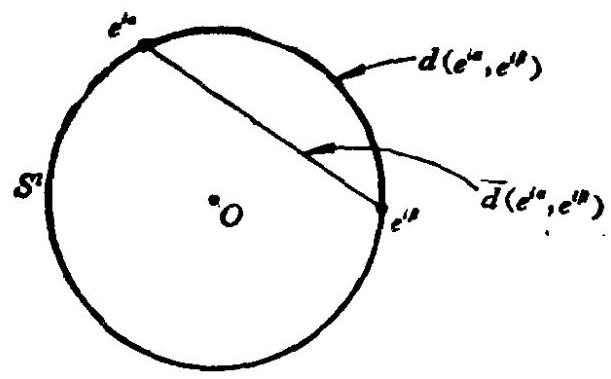
\includegraphics[max width=0.5\textwidth]{images/bo_d25ksc77aajc738obdgg_488_407_459_611_379_0.jpg}
\end{center}
\hspace*{3em} 

图 10-1

由上面例 1 与例 3 知, ${\mathbf{R}}^{n}$ 与 ${S}^{1}$ 上有不止一个度量,实际上,如果集合 $X$ 有度量 $d$ ,则 $X$ 上的度量就不是唯一的,因为 $\forall \lambda  > 0$ , ${\lambda d}$ 也是 $X$ 上的一个度量,下面我们介绍度量之间关系的一个概念, 即度量的等价。

\section*{3. 度量的等价}

定义 设 $d$ 与 ${d}^{\prime }$ 是 $X$ 上的任意两个度量. 我们称 $d$ 与 ${d}^{\prime }$ 是等价的,如果存在常数 $A > 0,B > 0$ 使得

$\forall x,y \in  X,{Ad}\left( {x,y}\right)  \leq  {d}^{\prime }\left( {x,y}\right)  \leq  {Bd}\left( {x,y}\right) .$

命题 ${\mathrm{R}}^{n}\left( {n > 1}\right)$ 上的三个基本度量 ${d}_{1},{d}_{2},{d}_{3}$ 是互相等价的, 并且成立下述不等式:
$$\forall x,y \in  {\mathbf{R}}^{n},{d}_{3}\left( {x,y}\right)  \leq  {d}_{1}\left( {x,y}\right)  \leq  {d}_{2}\left( {x,y}\right)  \leq  n{d}_{3}\left( {x,y}\right) .$$

证明 $\forall x,y \in  {\mathbf{R}}^{n}$ ,我们有
\begin{align*}
	&{d}_{3}\left( {x,y}\right)  = \max \left\{  {\left| {{x}_{1} - {y}_{1}}\right| ,\left| {{x}_{2} - {y}_{2}}\right| ,\cdots ,\left| {{x}_{n} - {y}_{n}}\right| }\right\}\\
	&= \left| {{x}_{k} - {y}_{k}}\right| \text{ (对某一个 }k = 1,2,\cdots ,n\text{ ) }\\
	&\leq  \sqrt{{\left( {x}_{1} - {y}_{1}\right) }^{2} + {\left( {x}_{2} - {y}_{2}\right) }^{2} + \cdots  + {\left( {x}_{n} - {y}_{n}\right) }^{2}}\\
	&= {d}_{1}\left( {x,y}\right) ,\\
	&{d}_{1}\left( {x,y}\right)  = \sqrt{{\left( {x}_{1} - {y}_{1}\right) }^{2} + {\left( {x}_{2} - {y}_{2}\right) }^{2} + \cdots  + {\left( {x}_{n} - {y}_{n}\right) }^{2}}\\
	&\leq  \left| {{x}_{1} - {y}_{1}}\right|  + \left| {{x}_{2} - {y}_{2}}\right|  + \cdots  + \left| {{x}_{n} - {y}_{n}}\right|\\
	&= {d}_{2}\left( {x,y}\right) ,\\
	&{d}_{2}\left( {x,y}\right)  = \left| {{x}_{1} - {y}_{1}}\right|  + \left| {{x}_{2} - {y}_{2}}\right|  + \cdots  + \left| {{x}_{n} - {y}_{n}}\right|
\end{align*}
\begin{align*}
	&\leq  \mathop{\max }\limits_{{1 \leq  i \leq  n}}\left| {{x}_{i} - {y}_{i}}\right|  + \mathop{\max }\limits_{{1 \leq  i \leq  n}}\left| {{x}_{i} - {y}_{i}}\right|  + \cdots\\
	&+ \mathop{\max }\limits_{{1 \leq  i \leq  n}}\left| {{x}_{i} - {y}_{i}}\right|\\
	&= n{d}_{3}\left( {x,y}\right) ,
\end{align*}

因此
$${d}_{3}\left( {x,y}\right)  \leq  {d}_{1}\left( {x,y}\right)  \leq  {d}_{2}\left( {x,y}\right)  \leq  n{d}_{3}\left( {x,y}\right) ,\forall x,y \in  {\mathbf{R}}^{n}.$$

由此不等式即可推知 ${d}_{1},{d}_{2},{d}_{3}$ 是 ${\mathbf{R}}^{n}$ 上的三个互相等价的度量.

下面我们介绍一个特殊的度量空间.

\section*{4. 赋范向量空间}

定义 设 $\mathbf{K} = \mathbf{R}$ 或 $\mathbf{C},E$ 是任一 $\mathbf{K}$ 一向量空间,若存在一个映射 $\parallel  \cdot  \parallel  : E \rightarrow  \mathbf{R}$ ,它具有下述三个性质:

1) $\forall x \in  E,\parallel x\parallel  \geq  0,\parallel x\parallel  = 0 \Leftrightarrow  x = 0$ ;

2) $\forall x \in  E,\forall \lambda  \in  \mathbf{K},\parallel {\lambda x}\parallel  = \left| \lambda \right|  \cdot  \parallel x\parallel$ ;

3) $\forall x,y \in  E,\parallel x + y\parallel  \leq  \parallel x\parallel  + \parallel y\parallel$ .

则我们称 $\parallel  \cdot  \parallel$ 是 $E$ 上的一个范数, $\left( {E,\parallel  \cdot  \parallel }\right)$ 称为一个赋范向量空间, 或简称为赋范空间.

我们说赋范向量空间 $\left( {E,\parallel  \cdot  \parallel }\right)$ 是一个特殊的度量空间,是因为:

若我们定义映射 $d : E \times  E \rightarrow  \mathbf{R}$ 如下:
$$\forall x,y \in  E,d\left( {x,y}\right)  = \parallel x - y\parallel .$$

则 $d$ 是 $E$ 上的一个度量. 事实上,由范数 $\parallel  \cdot  \parallel$ 的性质推知

i) $\forall x,y \in  E,d\left( {x,y}\right)  = \parallel x - y\parallel  \geq  0$ ,且 $\parallel x - y\parallel  = 0$ ,当且仅当 $x - y = 0$ 即 $x = y$ .

ii) $\forall x,y \in  E,d\left( {x,y}\right)  = \parallel x - y\parallel  = \parallel  - \left( {y - x}\right) \parallel  = \left| {-1}\right|$  $\parallel y - x\parallel  = \parallel y - x\parallel  = d\left( {y,x}\right) .$
\begin{align*}
	&\text{ iii) }\forall x,y,z \in  E\text{ , }\\
	&d\left( {x,y}\right)  = \parallel x - y\parallel  \leq  \parallel x - z\parallel  + \parallel z - y\parallel\\
	&= d\left( {x,z}\right)  + d\left( {z,y}\right) .
\end{align*}

这个度量 $d$ 称为由 $E$ 的范数 $\parallel  \cdot  \parallel$ 诱导出来的度量,因此(E, d)是一个度量空间.

注意 由赋范空间 $\left( {E,\parallel  \cdot  \parallel }\right)$ 所诱导的度量空间(E, d)与一般度量空间(X, d)不同之处在于: $E$ 不是一般的非空集合,而是一个向量空间, 它的元素可以进行加、减、数乘运算, 而一般度量空间(X, d)中 $X$ 的元素未必能定义这些运算.

如果 $E$ 上可以定义范数,那末 $E$ 上的范数就不是唯一的,像在度量空间中一样, 也可以定义范数的等价概念.

定义 设 $\parallel  \cdot  \parallel$ 与 $\parallel  \cdot  \parallel \prime$ 是 $E$ 上的任意两个范数,我们称 $\parallel  \cdot  \parallel$ 与 $\parallel  \cdot  {\parallel }^{\prime }$ 是等价的,如果存在常数 $A > 0,B > 0$ 使得
$$\forall x \in  E,A\parallel x\parallel  \leq  \parallel x\parallel \prime  \leq  B\parallel x\parallel .$$

最简单的赋范向量空间是下面两个例子.

例 4 设 $E = \mathbf{C},\forall z \in  \mathbf{C}$ ,令

$\parallel z\parallel  = \left| z\right|$ (复数 $z$ 的模).

容易验证如此定义的 $\parallel  \cdot  \parallel$ 是 $\mathrm{C}$ 上的一个范数.

因此 $\left( {\mathrm{C},\parallel  \cdot  \parallel }\right)$ 是一个赋范向量空间.

例5 设 $E = {\mathbf{R}}^{n}\left( {n \geq  1}\right) ,\forall x = \left( {{x}_{1},{x}_{2},\cdots ,{x}_{n}}\right)  \in  {\mathbf{R}}^{n}$ ,令
\begin{align*}
	&\parallel x{\parallel }_{1} = \sqrt{{x}_{1}^{2} + {x}_{2}^{2} + \cdots  + {x}_{n}^{2}},\\
	&\parallel x{\parallel }_{2} = \left| {x}_{1}\right|  + \left| {x}_{2}\right|  + \cdots  + \left| {x}_{n}\right| ,\\
	&\parallel x{\parallel }_{3} = \max \left\{  {\left| {x}_{1}\right| ,\;\left| {x}_{2}\right| ,\cdots ,\left| {x}_{n}\right| }\right\}  ,
\end{align*}

则 $\parallel  \cdot  {\parallel }_{i}\left( {i = 1,2,3}\right)$ 是 ${\mathbf{R}}^{n}$ 上的范数,因此 $\left( {{\mathbf{R}}^{n},\parallel  \cdot  {\parallel }_{i}}\right)$ 是赋范向量空间, 并且成立下述不等式:
$$\forall x \in  {\mathbf{R}}^{n},\parallel x{\parallel }_{3} \leq  \parallel x{\parallel }_{1} \leq  \parallel x{\parallel }_{2} < n\parallel x{\parallel }_{3}.$$

从而 $\parallel  \cdot  {\parallel }_{1},\parallel  \cdot  {\parallel }_{2},\parallel  \cdot  {\parallel }_{3}$ 是 ${\mathrm{R}}^{n}$ 上的三个互相等价的范数,我们称这三个范数为 ${\mathbf{R}}^{n}$ 上的基本范数.

上述结论的证明是容易的, 我们留给读者.

下面我们再举两个今后常见的赋范向量空间的例子.

例 6 设 ${C}^{0}\left( {\left\lbrack  {a,b}\right\rbrack  ,\mathrm{C}}\right)$ 为所有定义在 有限闭区间 $\left\lbrack  {a,b}\right\rbrack$ 上的连续复值函数的集合.

我们定义映射 $\parallel  \cdot  {\parallel }_{\infty } : {C}^{0}\left( {\left\lbrack  {a,b}\right\rbrack  ,\mathrm{C}}\right)  \rightarrow  \mathrm{R}$ 如下:
$$\forall f \in  {C}^{0}\left( {\left\lbrack  {a,b}\right\rbrack  ,\mathrm{C}}\right) ,\;\parallel f{\parallel }_{\infty } = \mathop{\sup }\limits_{{x \in  \left( {a,b}\right\rbrack  }}\left| {f\left( x\right) }\right| .$$

则 $\parallel  \cdot  {\parallel }_{\infty }$ 是 ${C}^{0}\left( {\left\lbrack  {a,b}\right\rbrack  ,\mathrm{C}}\right)$ 上的一个范数,因此 $\left( {{C}^{0}\left( {\left\lbrack  {a,b}\right\rbrack  ,\mathrm{C}}\right) }\right.$  $\parallel  \cdot  {\parallel }_{\infty }$ ) 是一个赋范向量空间.

首先我们证明映射 $\parallel  \cdot  {\parallel }_{\infty }$ 是有定义的,这是因为 $\forall f \in  {C}^{0}$  $\left( {\left\lbrack  {a,b}\right\rbrack  ,\mathbf{C}}\right)$ 由 $f$ 的连续性 及 $\left\lbrack  {a,b}\right\rbrack$ 的有限、闭性 知, $\mathop{\sup }\limits_{{x \in  \left\lbrack  {a,b}\right\rbrack  }}\left| f\right|$  $\left( x\right)  \mid   <  + \infty$ ,故 $\parallel f{\parallel }_{\infty } <  + \infty$ .

其次,若在 ${C}^{0}\left( {\left\lbrack  {a,b}\right\rbrack  ,\mathrm{C}}\right)$ 上定义加法与数乘运算为: $\forall f$ , $g \in  {C}^{0}\left( {\left\lbrack  {a,b}\right\rbrack  ,\mathrm{C}}\right) ,\;\forall \lambda  \in  \mathrm{C},$

$\forall x \in  \left\lbrack  {a,b}\right\rbrack  ,\left( {f + g}\right) \left( x\right)  = f\left( x\right)  + g\left( x\right) ,\left( {\lambda f}\right) \left( x\right)  = {\lambda f}\left( x\right) ,$ 则 ${C}^{0}\left( {\left\lbrack  {a,b}\right\rbrack  ,\mathbf{C}}\right)$ 关于这两个运算形成一个 $\mathbf{C}$ 一向量 空间.

下面我们来验证 $\parallel  \cdot  {\parallel }_{\infty }$ 是 ${C}^{0}\left( {\left\lbrack  {a,b}\right\rbrack  ,\mathrm{C}}\right)$ 上的范数.

1) $\forall f \in  {C}^{0}\left( {\left\lbrack  {a,b}\right\rbrack  ,\mathrm{C}}\right) ,\parallel f{\parallel }_{\infty } \geq  0$ ,并且 $\parallel f{\parallel }_{\infty } = 0 \Leftrightarrow$  $\mathop{\sup }\limits_{{x \in  \left\lbrack  {a;b}\right\rbrack  }}\left| {f\left( x\right) }\right|  = 0 \Leftrightarrow  \forall x \in  \left\lbrack  {a,b}\right\rbrack  ,\left| {f\left( x\right) }\right|  = 0 \Leftrightarrow  f = 0.$

2) $\forall f \in  {C}^{0}\left( {\left\lbrack  {a,b}\right\rbrack  ,C}\right) ,\forall \lambda  \in  \mathbf{R}$ ,
$$\parallel {\lambda f}{\parallel }_{\infty } = \mathop{\sup }\limits_{{x \in  \left\lbrack  {a,b}\right\rbrack  }}\left| {{\lambda f}\left( x\right) }\right|  = \left| \lambda \right| \mathop{\sup }\limits_{{x \in  \left\lbrack  {a,b}\right\rbrack  }}\left| {f\left( x\right) }\right|  = \left| \lambda \right| \parallel f{\parallel }_{\infty }.$$

3) $\forall f,g \in  {C}^{0}\left( {\left\lbrack  {a,b}\right\rbrack  ,C}\right)$ ,
\begin{align*}
	&\parallel f + g\parallel \underset{x \in  \left\lbrack  {a;b}\right\rbrack  }{ = }\left| {f\left( x\right)  + g\left( x\right) }\right|  \leq  \mathop{\sup }\limits_{{x \in  \left\lbrack  {a;b}\right\rbrack  }}\left| {f\left( x\right) }\right|  + \mathop{\sup }\limits_{{x \in  \left\lbrack  {a;b}\right\rbrack  }}\left| {g\left( x\right) }\right|\\
	&= \parallel f{\parallel }_{\infty } + \parallel g{\parallel }_{\infty }\text{ . }
\end{align*}

因此 $\parallel  \cdot  {\parallel }_{\infty }$ 的确是 ${C}^{0}\left( {\left\lbrack  {a,b}\right\rbrack  ,\mathbb{C}}\right)$ 上的一个范数,这个范数也称为 ${C}^{0}\left( {\left\lbrack  {a,b}\right\rbrack  ,\mathrm{C}}\right)$ 上的一致收敛范数,为什么称 $\parallel  \cdot  {\parallel }_{\infty }$ 为一致收敛范数,我们将在第 12 章进行解释.

例7 设 $\mathcal{L}\left( {{\mathbf{R}}^{n},{\mathbf{R}}^{m}}\right)$ 是所有从 ${\mathbf{R}}^{n}$ 到 ${\mathbf{R}}^{m}$ 的线性映射的集合, 在 ${\mathbf{R}}^{n}$ 与 ${\mathbf{R}}^{m}$ 上各自取定三个基本范数中的一个.

我们定义映射 $\parallel  \cdot  \parallel  : \mathcal{L}\left( {{\mathbf{R}}^{n},{\mathbf{R}}^{m}}\right)  \rightarrow  \mathbf{R}$ 如下:
$$\forall T \in  \mathcal{L}\left( {{\mathbf{R}}^{n},{\mathbf{R}}^{m}}\right) ,\parallel T\parallel  = \mathop{\sup }\limits_{{x \in  {\mathbf{R}}^{n},\parallel x\parallel  = 1}}\parallel T\left( x\right) \parallel .$$

则 $\begin{Vmatrix}\cdot \end{Vmatrix}$ 是 $\mathcal{L}\left( {{\mathbf{R}}^{n},{\mathbf{R}}^{m}}\right)$ 上的一个范数,因此 $\left( {\mathcal{L}\left( {{\mathbf{R}}^{n},{\mathbf{R}}^{m}}\right) ,\parallel  \cdot  \parallel }\right)$ 是一个赋范向量空间.

为方便起见,我们在 ${\mathbf{R}}^{n}$ 中取基本范数 $\parallel  \cdot  {\parallel }_{2}$ .

首先我们容易验证 $\mathcal{L}\left( {{\mathbf{R}}^{n},{\mathbf{R}}^{m}}\right)$ 是一个 $\mathbf{R}$ 一向量空间.

其次,我们证明映射 $\parallel  \cdot  \parallel$ 有定义,也即
$$\forall T \in  \mathcal{L}\left( {{\mathbf{R}}^{n},{\mathbf{R}}^{m}}\right) ,\parallel T\parallel  = \mathop{\sup }\limits_{{x \in  {\mathbf{R}}^{n} : \parallel x{\parallel }_{2} = 1}}\parallel T\left( x\right) \parallel  <  + \infty .$$

事实上,设 $\left( {{e}_{1},{e}_{2},\cdots ,{e}_{n}}\right)$ 是 ${\mathrm{R}}^{n}$ 的标准基底. 则 $\forall x = \left( {x}_{1}\right.$ , $\left. {{x}_{2},\cdots ,{x}_{n}}\right)  \in  {\mathrm{R}}^{n}$ ,我们有
$$x = {x}_{1}{e}_{1} + {x}_{2}{e}_{2} + \cdots  + {x}_{n}{e}_{n}.$$

若 $\parallel x{\parallel }_{2} = 1$ ,则 $\left| {x}_{1}\right|  + \left| {x}_{2}\right|  + \cdots  + \left| {x}_{n}\right|  = 1$ ,从而由 $T$ 的线性性及范数的性质, 我们有
\begin{align*}
	&\parallel T\left( x\right) \parallel  = \begin{Vmatrix}{T\left( {{x}_{1}{e}_{1} + {x}_{2}{e}_{2} + \cdots  + {x}_{n}{e}_{n}}\right) }\end{Vmatrix}\\
	&= \begin{Vmatrix}{{x}_{1}T\left( {e}_{1}\right)  + {x}_{2}T\left( {e}_{2}\right)  + \cdots  + {x}_{n}T\left( {e}_{n}\right) }\end{Vmatrix}\\
	&\leq  \left| {x}_{1}\right| \begin{Vmatrix}{T\left( {e}_{1}\right) }\end{Vmatrix} + \left| {x}_{2}\right| \begin{Vmatrix}{T\left( {e}_{2}\right) }\end{Vmatrix} + \cdots\\
	&+ \left| {x}_{n}\right| \begin{Vmatrix}{T\left( {e}_{n}\right) }\end{Vmatrix}\text{ . }
\end{align*}

令 $M = \max \left\{  {\begin{Vmatrix}{T\left( {e}_{1}\right) }\end{Vmatrix},\begin{Vmatrix}{T\left( {e}_{2}\right) ,}\end{Vmatrix}\cdots ,\begin{Vmatrix}{T\left( {e}_{n}\right) }\end{Vmatrix}}\right\}$ ,则 $M <  + \infty$ , 并且
$$\parallel T\left( x\right) \parallel  \leq  M\left( {\left| {x}_{1}\right|  + \left| {x}_{2}\right|  + \cdots  + \left| {x}_{n}\right| }\right)  = M.$$

最后我们来验证 $\parallel  \cdot  \parallel$ 满足范数的三个条件.

1) $\forall T \in  \mathcal{L}\left( {{\mathbf{R}}^{n},{\mathbf{R}}^{m}}\right) ,\parallel T\parallel  \geq  0$ 显然,下证 $\parallel T\parallel  = 0 \Leftrightarrow$  $T = 0$ .

设 $T = 0$ ,由 $\parallel T\parallel$ 的定义知 $\parallel T\parallel  = 0$ .

反之设 $\parallel T\parallel  = 0$ ,那末
\begin{align*}
	&\mathop{\sup }\limits_{{x \in  {\mathrm{R}}^{n};\parallel x\parallel  = 1}}\parallel T\left( x\right) \parallel  = 0 \Leftrightarrow  \forall x \in  {\mathbf{R}}^{n},\parallel x\parallel  = 1,\\
	&\parallel T\left( x\right) \parallel  = 0.
\end{align*}

现任取 $x \in  {\mathbf{R}}^{n}$ 且 $x \neq  0$ ,则 $\frac{x}{\parallel x\parallel } \in  {\mathbf{R}}^{n},\begin{Vmatrix}\frac{x}{\parallel x\parallel }\end{Vmatrix} = 1$ ,于是

$\begin{Vmatrix}{T\left( \frac{x}{\parallel x\parallel }\right) }\end{Vmatrix} = 0$ ,从而 $\parallel T\left( x\right) \parallel  = 0 \cdot  \parallel x\parallel  = 0$ .

若 $x \in  {\mathbf{R}}^{n}$ 且 $x = 0$ ,则显然有 $\parallel T\left( x\right) \parallel  = 0$ .

因此 $\forall x \in  {\mathbf{R}}^{n},\parallel T\left( x\right) \parallel  = 0$ ,此即表明 $T\left( x\right)  = 0$ 或 $T = 0$ .

2) $\forall T \in  \mathcal{L}\left( {{\mathbf{R}}^{n},{\mathbf{R}}^{m}}\right) ,\forall \lambda  \in  \mathbf{R},\parallel {\lambda T}\parallel  = \left| \lambda \right| \parallel T\parallel$ .

这可由 $\parallel T\parallel$ 的定义直接推出.

3) $\forall T,S \in  \mathcal{L}\left( {{\mathbf{R}}^{n},{\mathbf{R}}^{m}}\right) ,\parallel T + S\parallel  \leq  \parallel T\parallel  + \parallel S\parallel$ . 这是因为
\begin{align*}
	&\parallel T + S\parallel  = \mathop{\sup }\limits_{{x \in  {\mathrm{R}}^{n};\parallel x\parallel  = 1}}\parallel \left( {T + S}\right) \left( x\right) \parallel\\
	&\leq  \mathop{\sup }\limits_{{x \in  {\mathrm{R}}^{n};\parallel x\parallel  = 1}}\parallel T\left( x\right) \parallel  + \mathop{\sup }\limits_{{x \in  {\mathrm{R}}^{n};\parallel x\parallel  = 1}}\parallel S\left( x\right) \parallel\\
	&= \parallel T\parallel  + \parallel S\parallel .
\end{align*}

因此上述定义的 $\parallel  \cdot  \parallel$ 是 $\mathcal{L}\left( {{\mathbf{R}}^{n},{\mathbf{R}}^{m}}\right)$ 上的一个范数.

由范数的定义, 我们得到下述不等式.

重要不等式 $\forall T \in  \mathcal{L}\left( {{\mathbf{R}}^{n},{\mathbf{R}}^{m}}\right) ,\forall x \in  {\mathbf{R}}^{n}$ ,
$$\parallel T\left( x\right) \parallel  \leq  \parallel T\parallel  \cdot  \parallel x\parallel .$$

注意这个不等式左、右 两 边的三个 $\parallel  \cdot  \parallel$ 代表三个不同空间中的范数.

此不等式的证明简单. $\forall x \in  {\mathbf{R}}^{n}$ ,且 $x \neq  0$ ,我们有 $\begin{Vmatrix}{T\left( \frac{x}{\parallel x\parallel }\right) }\end{Vmatrix} \leq  \parallel T\parallel$ ,从而 $\parallel T\left( x\right) \parallel  \leq  \parallel T\parallel  \cdot  \parallel x\parallel$ . 若 $x \in  {\mathbf{R}}^{n}$ 且 $x = 0$ ,则 $\parallel T\left( x\right) \parallel  = 0 = \parallel T\parallel  \cdot  \parallel x\parallel$ . 因此
$$\forall x \in  {\mathbf{R}}^{n},\parallel T\left( x\right) \parallel  \leq  \parallel T\parallel  \cdot  \parallel x\parallel .$$

\section*{习 题}

1. 设 $X$ 是任一非空集合,定义映射 $d : X \times  X \rightarrow  R$ 如下:
$$\forall x,y \in  X,d\left( {x,y}\right)  = \left\{  \begin{array}{ll} 0, & \text{ 若 }x = y, \\  1, & \text{ 若 }x \neq  y. \end{array}\right.$$

证明: $d$ 是 $X$ 上的一个度量.

2. 设 $X$ 是任一非空集合, $f : X \rightarrow  R$ 是任一单射. 证明:映射 $d : X \times  X \rightarrow  R$
$$\forall x,y \in  X,d\left( {x,y}\right)  = \left| {f\left( x\right)  - f\left( y\right) }\right|$$

是 $X$ 上的一个度量.

3. 设(X, d)是任一度量空间. 令
$$\bar{d}\left( {x,y}\right)  = \min \left( {d\left( {x,y}\right) ,1}\right) ,\forall x,y \in  \mathbf{X},$$

证明: $\bar{d}$ 是 $X$ 上的一个度量.

4. 设 ${C}^{2}\left( {\left\lbrack  {0,1}\right\rbrack  ,\mathrm{R}}\right)$ 表示所有定义在 $\left\lbrack  {0,1}\right\rbrack$ 上的2次连续可导函数的集合.

1) $\forall f,g \in  {C}^{2}\left( {\left\lbrack  {0,1}\right\rbrack  ,R}\right)$ ,我们令
\begin{align*}
	&{d}_{1}\left( {f,g}\right)  = \mathop{\sup }\limits_{{x \in  \left\lbrack  {0;1}\right\rbrack  }}\left| {f\left( x\right)  - g\left( x\right) }\right| ,\\
	&{d}_{2}\left( {f,g}\right)  = \mathop{\sup }\limits_{{x \in  \left\lbrack  {0;1}\right\rbrack  }}\left| {{f}^{\prime }\left( x\right)  - {g}^{\prime }\left( x\right) }\right|  + \left| {f\left( 0\right)  - g\left( 0\right) }\right| ,\\
	&{d}_{3}\left( {f,g}\right)  = \mathop{\sup }\limits_{{x \in  \left\lbrack  {0;1}\right\rbrack  }}\left| {{f}^{\prime \prime }\left( x\right)  - {g}^{\prime \prime }\left( x\right) }\right|  + \left| {{f}^{\prime }\left( 0\right)  - {g}^{\prime }\left( 0\right) }\right|\\
	&+ \left| {f\left( 0\right)  - g\left( 0\right) }\right| \text{ , }
\end{align*}

证明: ${d}_{1},{d}_{2},{d}_{3}$ 是 ${C}^{2}(\left\lbrack  {0,1}\right\rbrack  ,\mathrm{R})$ 上的度量.

2) 证明: $\forall f,g \in  {C}^{2}\left( {\left\lbrack  {0,1}\right\rbrack  ,R}\right)$
$${d}_{1}\left( {f,g}\right)  \leq  {d}_{2}\left( {f,g}\right)  \leq  {d}_{3}\left( {f,g}\right) .$$

5. 设 $G$ 是任一交换群. $p : G \rightarrow  {R}^{ + }$ 是任一映射,它满足下述条件:
$$p\left( x\right)  = 0 \Leftrightarrow  x = 0,p\left( {-x}\right)  = p\left( x\right) ,p\left( {x + y}\right)  \leq  p\left( x\right)  + p\left( y\right) .$$

证明: $d : G \times  G \rightarrow  R$
$$d\left( {x,y}\right)  = p\left( {x - y}\right) ,\;\forall \left( {x,y}\right)  \in  G \times  G$$

是 $G$ 上的一个度量.

6. 设(X, d)是任一度量空间.

1) 证明: ${d}^{\prime } = \frac{d}{1 + d}$ 是 $X$ 上的一个度量.

2) 证明: ${d}^{\prime }$ 与第 3 题中的度量 $\bar{d}$ 是等价度量,并且满足不等式 ${d}^{\prime } \leq$  $\bar{d} \leq  2{d}^{\prime }$ .

7. 设 $p \geq  1$ ,在 ${R}^{n}$ 上定义映射 ${N}_{p} : {R}^{n} \rightarrow  {R}^{ + }$ 如下:
$$\forall x = \left( {{x}_{1},{x}_{2},\cdots ,{x}_{n}}\right)  \in  {R}^{n},{N}_{p}\left( x\right)  = {\left( {\left| {x}_{1}\right| }^{p} + {\left| {x}_{2}\right| }^{p} + \cdots  + {\left| {x}_{n}\right| }^{p}\right) }^{\frac{1}{p}}.$$

1) 证明: ${N}_{\mathfrak{p}}$ 是 ${R}^{n}$ 上的一个范数,称为 ${l}_{\mathfrak{p}}$ 范数

2) 证明: 范数 ${N}_{p}$ 与 ${R}^{n}$ 的三个基本范数等价.

8. 设 $\parallel  \cdot  \parallel$ 是 ${R}^{n}$ 上的任一范数, $x,y \in  {R}^{n}$ ,若
$$\parallel x + y\parallel  = \parallel x\parallel  + \parallel y\parallel ,$$

则 $x$ 与 $y$ 应满足什么关系?

9. 设 $N$ 与 ${N}^{\prime }$ 分别是 ${\mathrm{R}}^{n}$ 与 ${\mathrm{R}}^{m}$ 的任一范数,在 ${\mathrm{R}}^{n + m} = {\mathrm{R}}^{n} \times  {\mathrm{R}}^{m}$ 上分别定又映射 ${N}_{1},{N}_{2},{N}_{3} : {R}^{n + m} \rightarrow  {R}^{ + }$ 如下:
\begin{align*}
	&\forall \left( {x,y}\right)  \in  {\mathbf{R}}^{n} \times  {\mathbf{R}}^{m} = {\mathbf{R}}^{n + m},{N}_{1}\left( {x,y}\right)  = \sqrt{{\left( N\left( x\right) \right) }^{2} + {\left( {N}^{\prime }\left( y\right) \right) }^{2}},\\
	&{N}_{2}\left( {x,y}\right)  = N\left( x\right)  + {N}^{\prime }\left( y\right) ,\\
	&{N}_{3}\left( {x,y}\right)  = \max \left\{  {N\left( x\right) ,{N}^{\prime }\left( y\right) }\right\}  .
\end{align*}

证明: ${N}_{1},{N}_{2},{N}_{3}$ 是 ${R}^{n + m}$ 上的三个范数.

10. 在 ${C}^{0}\left( {\left\lbrack  {a,b}\right\rbrack  ,R}\right)$ 上定义映射 ${N}_{1},{N}_{2} : {C}^{0}\left( {\left\lbrack  {a,b}\right\rbrack  ,R}\right)  \rightarrow  {R}^{ * }$ 如下:
\begin{align*}
	&\forall f \in  {C}^{0}\left( {\left\lbrack  {a,b}\right\rbrack  ,\mathrm{R}}\right) ,{N}_{1}\left( f\right)  = {\int }_{a}^{b}\left| {f\left( x\right) }\right| {dx},\\
	&{N}_{2}\left( f\right)  = {\left( {\int }_{a}^{b}{f}^{2}\left( x\right) dx\right) }^{\frac{1}{2}}.
\end{align*}

证明: ${N}_{1}$ 与 ${N}_{2}$ 是 ${C}^{0}\left( {\left\lbrack  {a,b}\right\rbrack  ,R}\right)$ 上的两个范数,它们是等价范数吗? 11. 在 ${C}^{1}\left( {\left\lbrack  {a,b}\right\rbrack  ,R}\right)$ 上定义映射 ${N}_{1},{N}_{2} : {C}^{1}\left( {\left\lbrack  {a,b}\right\rbrack  ,R}\right)  \rightarrow  {R}^{ + }$ 如下: $\forall f \in  {C}^{1}\left( {\left\lbrack  {a,b}\right\rbrack  ,\mathrm{R}}\right) ,{N}_{1}\left( f\right)  = \mathop{\sup }\limits_{{x \in  \left\lbrack  {a;b}\right\rbrack  }}\left| {f\left( x\right) }\right|  + \mathop{\sup }\limits_{{x \in  \left\lbrack  {a;b}\right\rbrack  }}\left| {{f}^{\prime }\left( x\right) }\right| ,$
$${N}_{2}\left( f\right)  = \mathop{\sup }\limits_{{x \in  \left\lbrack  {a;b}\right\rbrack  }}\left( {\left| {f\left( x\right) }\right|  + \left| {{f}^{\prime }\left( x\right) }\right| }\right) .$$

证明: ${N}_{1}$ 与 ${N}_{2}$ 是 ${C}^{1}\left( {\left\lbrack  {a,b}\right\rbrack  ,R}\right)$ 上的两个等价范数. 12. 明: 1) 对 $i{d}_{{R}^{n}} \in  \mathcal{L}\left( {{R}^{n},{R}^{n}}\right) ,\begin{Vmatrix}{i{d}_{{R}^{n}}}\end{Vmatrix} = 1$ , 2) $\forall T \in  \mathcal{L}\left( {{R}^{n},{R}^{m}}\right) ,\forall S \in  \mathcal{L}\left( {{R}^{m},{R}^{k}}\right) ,\parallel S \circ  T\parallel  \leq  \parallel S\parallel  \cdot  \parallel T\parallel$ .

\section{度量空间的开集、闭集}

为了进一步认识度量空间, 我们来介绍度量空间的开集、闭集及其基本性质.

\section*{1. 开球、闭球及球面}

定义 设(X, d)是任一度量空间, $\forall a \in  X,\forall \delta  \geq  0$ ,我们令
\begin{align*}
	&B\left( {a,\delta }\right) \text{ ① } = \{ x \in  X \mid  d\left( {a,x}\right)  < \delta \} ,\\
	&\bar{B}\left( {a,\delta }\right)  = \{ x \in  X \mid  d\left( {a,x}\right)  \leq  \delta \} ,\\
	&S\left( {a,\delta }\right)  = \{ x \in  X \mid  d\left( {a,x}\right)  = \delta \} ,
\end{align*}

\footnote{
	
	① 有时为了指明度量 $d$ ,我们也采用记号 ${B}_{d}\left( {a,\delta }\right) ,{B}_{d}\left( {a,\delta }\right) ,{S}_{d}\left( {a,\delta }\right)$ .
	
}

并分别称 $B\left( {a,\delta }\right)$ 、 $\bar{B}\left( {a,\delta }\right)$ 及 $S\left( {a,\delta }\right)$ 为 $X$ 的以 $a$ 为中心,以 $\delta$ 为半径的开球、闭球及球面.

在赋范向量空间 $\left( {E,\parallel  \cdot  \parallel }\right)$ 中,相应地我们有
\begin{align*}
	&B\left( {a,\delta }\right)  = \{ x \in  E \mid  \parallel x - a\parallel  < \delta \} ,\\
	&\bar{B}\left( {a,\delta }\right)  = \{ x \in  E \mid  \parallel x - a\parallel  \leq  \delta \} ,\\
	&S\left( {a,\delta }\right)  = \{ x \in  E \mid  \parallel x - a\parallel  = \delta \} .
\end{align*}

注意 若 $\delta  = 0$ ,则 $B\left( {a,\delta }\right)  = \varnothing ,\bar{B}\left( {a,\delta }\right)  = S\left( {a,\delta }\right)  = \{ a\}$ . 若 $\delta  > 0$ ,则 $a \in  B\left( {a,\delta }\right)  \subset  \bar{B}\left( {a,\delta }\right)$ ,并且
$$B\left( {a,\delta }\right)  \cup  S\left( {a,\delta }\right)  = \bar{B}\left( {a,\delta }\right) .$$

例1 设 $X = \mathbf{R},d\left( {x,y}\right)  = \left| {x - y}\right|$ 为绝对值度量,于是

$B\left( {a,\delta }\right)  = \rbrack a - \delta ,a + \delta \lbrack ,\bar{B}\left( {a,\delta }\right)  = \left\lbrack  {a - \delta ,a + \delta }\right\rbrack  ,$
$$S\left( {a,\delta }\right)  = \{ a - \delta ,a + \delta \} .$$

例2 设 $X = {\mathbf{R}}^{2}$ . 我们来考虑在 ${\mathbf{R}}^{2}$ 的三个基本度量 ${d}_{1},{d}_{2}$ , ${d}_{3}$ 下的 $B\left( {a,\delta }\right) ,\bar{B}\left( {a,\delta }\right)$ 与 $S\left( {a,\delta }\right)$ .

记 $a = \left( {{a}_{1},{a}_{2}}\right) ,x = \left( {{x}_{1},{x}_{2}}\right)$ .

1) 对度量 ${d}_{1}$ :
\begin{align*}
	&B\left( {a,\delta }\right)  = \left\{  {x \in  {\mathbf{R}}^{2} \mid  \sqrt{{\left( {x}_{1} - {a}_{1}\right) }^{2} + {\left( {x}_{2} - {a}_{2}\right) }^{2}} < \delta }\right\}  ,\\
	&\bar{B}\left( {a,\delta }\right)  = \left\{  {x \in  {\mathbf{R}}^{2} \mid  \sqrt{{\left( {x}_{1} - {a}_{1}\right) }^{2} + {\left( {x}_{2} - {a}_{2}\right) }^{2}} \leq  \delta }\right\}  ,\\
	&S\left( {a,\delta }\right)  = \left\{  {x \in  {\mathbf{R}}^{2} \mid  \sqrt{{\left( {x}_{1} - {a}_{1}\right) }^{2} + {\left( {x}_{2} - {a}_{2}\right) }^{2}} = \delta }\right\}  .
\end{align*}

这里 $B\left( {a,\delta }\right) ,\bar{B}\left( {a,\delta }\right) ,S\left( {a,\delta }\right)$ 就 是平面上通常所说的以 $a$ 为中心 $\delta$ 为半径的开圆盘、闭圆盘、圆周.

2) 对度量 ${d}_{2}$ :
\begin{align*}
	&B\left( {a,\delta }\right)  = \left\{  {x \in  {\mathbf{R}}^{2}\left| \right| {x}_{1} - {a}_{1}\left| +\right| {x}_{2} - {a}_{2} \mid   < \delta }\right\}  ,\\
	&\bar{B}\left( {a,\delta }\right)  = \left\{  {x \in  {\mathbf{R}}^{2}\left| \right| {x}_{1} - {a}_{1}\left| +\right| {x}_{2} - {a}_{2} \mid   \leq  \delta }\right\}  ,\\
	&S\left( {a,\delta }\right)  = \left\{  {x \in  {\mathbf{R}}^{2}\left| \right| {x}_{1} - {a}_{1}\left| +\right| {x}_{2} - {a}_{2} \mid   = \delta }\right\}  .
\end{align*}

这时 $B\left( {a,\delta }\right) ,\bar{B}\left( {a,\delta }\right) ,S\left( {a,\delta }\right)$ 是平面上以 $a$ 为中心,两

条对角线分别平行于 ${x}_{1}$ 轴与 ${x}_{2}$ 轴而长为 ${2\delta }$ 的开菱形、闭菱形、四

\begin{center}
	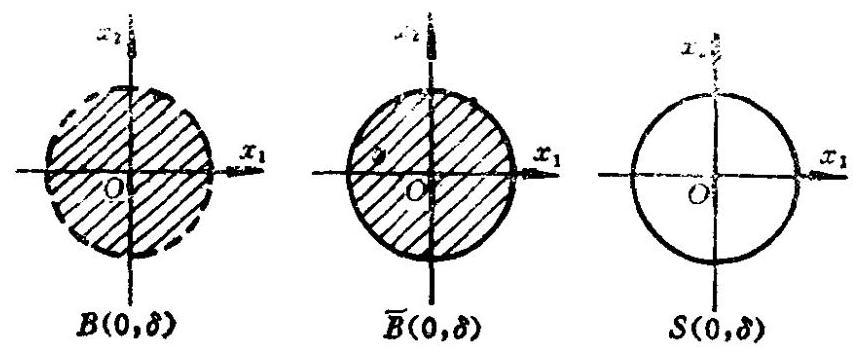
\includegraphics[max width=0.7\textwidth]{images/bo_d25ksc77aajc738obdgg_497_387_269_862_355_0.jpg}
\end{center}
\hspace*{3em} 

图 10-2

\begin{center}
	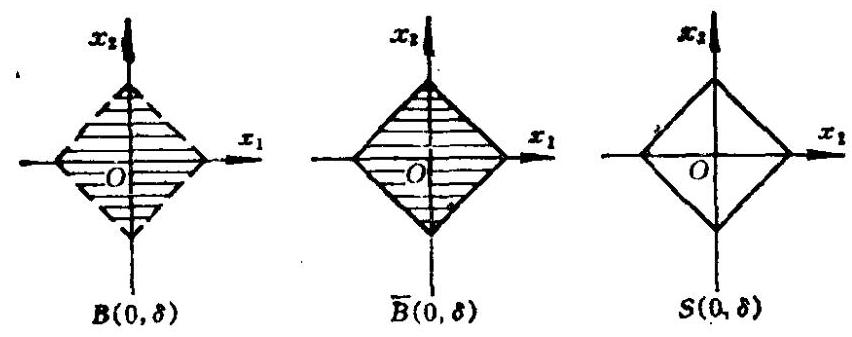
\includegraphics[max width=0.7\textwidth]{images/bo_d25ksc77aajc738obdgg_497_422_724_852_337_0.jpg}
\end{center}
\hspace*{3em} 

图 10-3

\section*{条菱边.}

3) 对度量 ${d}_{3}$ :
\begin{align*}
	&B\left( {a,\delta }\right)  = \left\{  {x \in  {\mathbf{R}}^{2}\left| {\max \left\{  {\left| {{x}_{1} - {a}_{1}}\right| ,}\right\}  {x}_{2} - {a}_{2}}\right|  < \delta }\right\}  ,\\
	&\bar{B}\left( {a,\delta }\right)  = \left\{  {x \in  {\mathbf{R}}^{2}\left| {\max \left\{  {\left| {{x}_{1} - {a}_{1}}\right| ,}\right\}  }\right| {x}_{2} - {a}_{2} \mid  }\right\}   \leq  \delta \} ,\\
	&S\left( {a,\delta }\right)  = \left\{  {x \in  {\mathbf{R}}^{2} \mid  \max \left\{  {\left| {{x}_{1} - {a}_{1}}\right| ,\left| {{x}_{2} - {a}_{2}}\right| }\right\}   = \delta }\right\}  .
\end{align*}

显然这里 $B\left( {a,\delta }\right) ,\bar{B}\left( {a,\delta }\right) ,S\left( {a,\delta }\right)$ 是平面上以 $a$ 为中心、两对边分别平行于 ${x}_{1}$ 轴与 ${x}_{2}$ 轴而长为 ${2\delta }$ 的开正方形、闭正方形、正方形四条边.

\begin{center}
	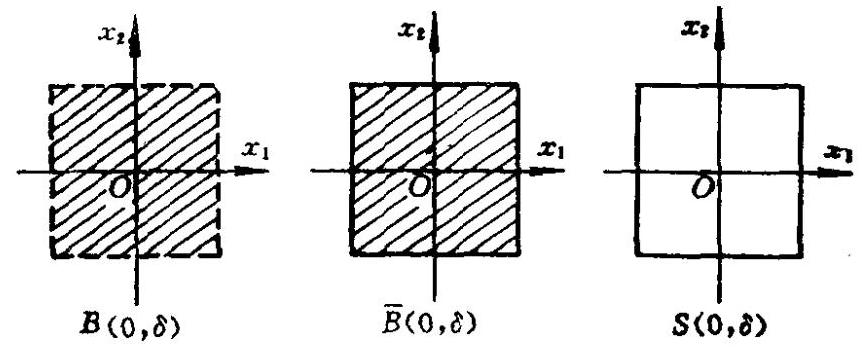
\includegraphics[max width=0.7\textwidth]{images/bo_d25ksc77aajc738obdgg_497_414_1631_862_348_0.jpg}
\end{center}
\hspace*{3em} 

图 10-4

由此可知,在同 $- X$ 上,对不同的度量 $d,B\left( {a,\delta }\right) ,B\left( {a,\delta }\right)$ 与 $S\left( {a,\delta }\right)$ 可以有不同的几何形状.

\section*{2. 开集、闭集、邻域}

定义 设(X, d)是任一度量空间, $U \subset  X$ 是任一集合. $a \in  X$ .

1) 我们称 $U$ 是 $X$ 的开集,如果
$$\left( {\forall x \in  U}\right) \left( {\exists \delta  > 0}\right) \text{ 使得 }B\left( {x,\delta }\right)  \subset  U\text{ . }$$

2) 我们称 $U$ 是 $X$ 的闭集,如果 $X - U$ 是 $X$ 的开集.

3) 我们称 $U$ 是 $a$ 的一个邻域,如果 $U$ 是包含 $a$ 的开集. 我们用 $\mathcal{N}\left( a\right)$ 表示 $a$ 的所有邻域组成的集族,称为 $a$ 的邻域系.

由上述定义可知: 空集 $\varnothing$ 与 $X$ 本身既是开集又是闭集.

当然, 在度量空间中, 一般说来存在既非开又非闭的集合. 因此当 $A$ 不是(X, d)中的开 (闭) 集时,我们不能断定 $A$ 就一定是 (X, d)的闭 $\left( \text{ 开 }\right)$ 集.

例如熟知的半闭半开的区间 $\left\lbrack  {a,b\left\lbrack  ,\right\rbrack  a,b}\right\rbrack  (a,b \in  \mathbf{R}$ , $a \neq  b)$ 就是 $\left( {\mathbf{R},\left| \cdot \right| }\right)$ 中的既非开又非闭的集合. 最简单的开集、闭集

命题 设(X, d)是任一度量空间. 则

1) $X$ 的任一单点集 $\{ a\}$ 是闭集,

2) $X$ 的任一开球 $B\left( {a,\delta }\right)$ 是开集,

3) $X$ 的任一闭球 $\bar{B}\left( {a,\delta }\right)$ 是闭集.

证明 1) 为了证明 $\{ a\}$ 是闭集,只需证明 $X - \{ a\}$ 是开集. 事实上, $\forall x \in  X - \{ a\} ,d\left( {x,a}\right)  > 0$ ,若取 $\delta  = \frac{1}{2}d\left( {x,a}\right)$ ,则 $\delta  > 0,B\left( {x,\delta }\right)  \subset  X - \{ a\}$ . 因此 $X - \{ a\}$ 是 $X$ 的开集.

2) 对开球 $B\left( {a,\delta }\right)$ : 若 $\delta  = 0$ ,则 $B\left( {a,\delta }\right)  = \varnothing$ ,它是开集. 现假设 $\delta  > 0$ ,为了证明 $B\left( {a,\delta }\right)$ 是开集,我们来证明:

$\left( {\forall x \in  B\left( {a,\delta }\right) }\right) \left( {\exists {\delta }_{x} > 0}\right)$ 使得 $B\left( {x,{\delta }_{x}}\right)  \subset  B\left( {a,\delta }\right)$ .

事实上,由于 $x \in  B\left( {a,\delta }\right)$ ,故 $d\left( {x,a}\right)  < \delta$ . 令 ${\delta }_{x} = \delta  - d\left( {x,a}\right)$ , 则 ${\delta }_{x} > 0$ .

现在设 $y \in  B\left( {x,{\delta }_{x}}\right)$ ,于是
\begin{align*}
	&d\left( {a,y}\right)  \leq  d\left( {a,x}\right)  + d\left( {x,y}\right)  < d\left( {a,x}\right)  + {\delta }_{x}\\
	&= d\left( {a,x}\right)  + \delta  - d\left( {x,a}\right)  = \delta .
\end{align*}

此即表明 $y \in  B\left( {a,\delta }\right)$ ,从而 $B\left( {x,{\delta }_{x}}\right)  \subset  B\left( {a,\delta }\right)$ .

\begin{center}
	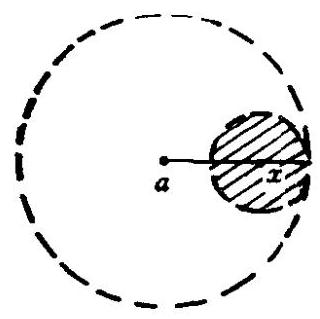
\includegraphics[max width=0.2\textwidth]{images/bo_d25ksc77aajc738obdgg_499_299_533_320_319_0.jpg}
\end{center}
\hspace*{3em} 

图 10-5

\begin{center}
	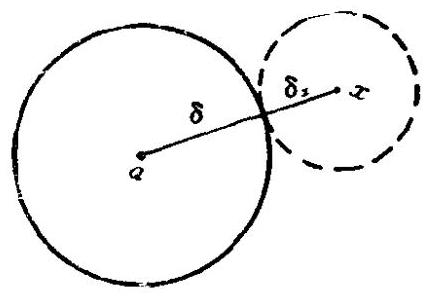
\includegraphics[max width=0.3\textwidth]{images/bo_d25ksc77aajc738obdgg_499_850_531_426_299_0.jpg}
\end{center}
\hspace*{3em} 

图 10-6

3) 对闭球 $\bar{B}\left( {a,\delta }\right)$ : 若 $\delta  = 0$ ,则 $\bar{B}\left( {a,\delta }\right)  = \{ a\}$ ,是闭集, 现假设 $\delta  > 0$ . 为了证明 $\bar{B}\left( {a,\delta }\right)$ 为闭集,我们证明 $X - \bar{B}\left( {a,\delta }\right)$ 为开集, 即等价地证明:

$\left( {\forall x \in  X - \bar{B}\left( {a,\delta }\right) }\right) \left( {\exists {\delta }_{x} > 0}\right)$ 使得 $B\left( {x,{\delta }_{x}}\right)  \subset  X - \bar{B}\left( {a,\delta }\right)$ .

事实上,由于 $x \in  \bar{B}\left( {a,\delta }\right)$ ,故 $d\left( {x,a}\right)  > \delta$ . 令 ${\delta }_{x} = d\left( {x,a}\right)  -$  $\delta$ ,则 ${\delta }_{x} > 0$ . 于是 $\forall y \in  B\left( {x,{\delta }_{x}}\right)$ ,
\begin{align*}
	&d\left( {y,a}\right)  \geq  d\left( {x,a}\right)  - d\left( {y,x}\right)\\
	&> d\left( {x,a}\right)  - d\left( {x,a}\right)  + \delta  = \delta .
\end{align*}

此即表明 $y \in  \bar{B}\left( {a,\delta }\right)$ ,因此 $y \in  X - \bar{B}\left( {a,\delta }\right)$ ,即 $B\left( {x,{\delta }_{x}}\right)  \subset$  $X - \bar{B}\left( {a,\delta }\right) .$

度量空间的一个重要性质就是它的Hausdorff分离性.

Hausdorff分离性

定理 ${10} \cdot  2 \cdot  1$ 设(X, d)是任一度量空间, $a,b \in  X$ 且 $a \neq  b$ . 则存在 $U \in  \mathcal{N}\left( a\right) ,V \in  \mathcal{N}\left( b\right)$ 使得
$$U \cap  V = \varnothing \text{ . }$$

证明 因为 $a \neq  b$ ,故 $d\left( {a,b}\right)  > 0$ ,取 $\delta  = \frac{1}{2}d\left( {a,b}\right)$ ,则

$B\left( {a,\delta }\right)  \in  \mathcal{V}\left( a\right) ,B\left( {b,\delta }\right)  \in  \mathcal{V}\left( b\right)$ ,并且
$$B\left( {a,\delta }\right)  \cap  B\left( {b,\delta }\right)  = \varnothing .$$

最后令 $U = B\left( {a,\delta }\right) ,V = B\left( {b,\delta }\right)$ 即可.

\section*{开集、闭集的性质}

定理 ${10} \cdot  2 \cdot  2$ 设(X, d)是任一度量空间,则

1) $X$ 的有限个开集的交是 $X$ 的开集,

2) $X$ 的任意一族开集的并是 $X$ 的开集.

证明 1) 设 ${U}_{i}\left( {i = 1,2,\cdots ,m}\right)$ 是 $X$ 的任意 $m$ 个开集,若 $\mathop{\bigcap }\limits_{{i = 1}}^{m}{U}_{i} = \varnothing$ ,则它是开集,因此不妨设 $\mathop{\bigcap }\limits_{{i = 1}}^{m}{U}_{i} \neq  \varnothing$ ,

$\forall x \in  \mathop{\bigcap }\limits_{{i = 1}}^{m}{U}_{i}$ ,由 $x \in  {U}_{i}$ 知,存在 ${\delta }_{i} > 0$ 使得
$$B\left( {x,{\delta }_{i}}\right)  \subset  {U}_{i}\;\left( {i = 1,2,\cdots ,m}\right) .$$

令 $\delta  = \min \left\{  {{\delta }_{1},{\delta }_{2},\cdots ,{\delta }_{m}}\right\}$ ,则 $\delta  > 0,B\left( {x,\delta }\right)  \subset  B\left( {x,{\delta }_{i}}\right)  \subset$  ${U}_{i}\left( {i = 1,2,\cdots ,m}\right)$ ,从而 $B\left( {x,\delta }\right)  \subset  \mathop{\bigcap }\limits_{{i = 1}}^{m}{U}_{i}$ ,因此 $\mathop{\bigcap }\limits_{{i = 1}}^{m}{U}_{i}$ 是 $X$ 的开集.

2) 设 ${\left\{  {U}_{\lambda }\right\}  }_{\lambda  \in  \Lambda }$ 是 $X$ 的任一开集族. 于是 $\forall x \in  \mathop{\bigcup }\limits_{{\lambda  \in  \Lambda }}{U}_{\lambda }$ ,存在 ${\lambda }_{0} \in  \Lambda$ ,存在 $\delta  > 0$ ,使得 $B\left( {x,\delta }\right)  \subset  {U}_{{\lambda }_{0}}$ ,从而 $B\left( {x,\delta }\right)  \subset  \mathop{\bigcup }\limits_{{\lambda  \in  \Lambda }}{U}_{\lambda }$ . 因此 $\mathop{\bigcup }\limits_{{\lambda  \in  \Lambda }}{U}_{\lambda }$ 是 $X$ 的开集.

定理 ${10} \cdot  2 \cdot  3$ 设(X, d)是任一度量空间,则

1) $X$ 的有限个闭集的并是 $X$ 的闭集,

2) $X$ 的任意一族闭集的交是 $X$ 的闭集.

证明 1) 设 ${F}_{i}\left( {i = 1,2,\cdots ,m}\right)$ 是 $X$ 的任意 $m$ 个闭集. 于是 $X - {F}_{i}\left( {i = 1,2,\cdots ,m}\right)$ 是 $X$ 的开集,从而由 De Morgan公式.
$$X - \mathop{\bigcup }\limits_{{i = 1}}^{m}{F}_{i} = \mathop{\bigcap }\limits_{{i = 1}}^{m}\left( {X - {F}_{i}}\right)$$

及定理 ${10} \cdot  2 \cdot  2$ 知 $X - \mathop{\bigcup }\limits_{{i = 1}}^{m}{F}_{i}$ 是 $X$ 的开集,因此 $\mathop{\bigcup }\limits_{{i = 1}}^{m}{F}_{i}$ 是 $X$ 的闭集.

2) 现设 ${\left\{  {F}_{\lambda }\right\}  }_{\lambda  \in  \Lambda }$ 是 $X$ 的任意一闭集族,由于 $\forall \lambda  \in  \Lambda ,X - {F}_{\lambda }$ 为 $X$ 的开集,故由 De Morgan公式
$$X - \mathop{\bigcap }\limits_{{\lambda  \in  \Lambda }}{F}_{\lambda } = \mathop{\bigcup }\limits_{{\lambda  \in  \Lambda }}\left( {X - {F}_{\lambda }}\right)$$

及定理 ${10} \cdot  2 \cdot  2$ 知 $X - \mathop{\bigcap }\limits_{{\lambda  \in  \Lambda }}{F}_{\lambda }$ 是 $X$ 的开集,从而交集 $\mathop{\bigcap }\limits_{{\lambda  \in  \Lambda }}{F}_{\lambda }$ 是 $X$ 的闭集.

现在我们用 $\tau$ 表示度量空间(X, d)的所有开集组成的集族, 由前面的讨论可知, $\tau$ 具有下述三个重要性质:

i) $\varnothing ,X \in  \tau$ ;

ii) 若 $U,V \in  \tau$ ,则 $U \cap  V \in  \tau$ ;

iii) 若 ${U}_{\lambda } \in  \tau \left( {\lambda  \in  \Lambda }\right)$ ,则 $\mathop{\bigcup }\limits_{{\lambda  \in  \Lambda }}{U}_{\lambda } \in  \tau$ .

我们称此开集族 $\tau$ 是由 $X$ 的度量 $d$ 诱导出来的一个拓扑 (Topology).

如果我们在一个集合 $X$ 上直接地给出满足上述i)、ii)、iii) 三个条件的 $X$ 上的一个集族 $\tau$ ,则我们称 $\tau$ 是 $X$ 上的一个拓扑, $U \in  \tau$ 称为开集, $\left( {X,\tau }\right)$ 称为一个拓扑空间,若这个拓扑是由 $X$ 上的某一个度量 $d$ 所诱导的,则称 $\left( {X,\tau }\right)$ 是可度量化拓扑空间. 这方面的内容属于专门的拓扑学的研究范畴,已超出. 书的范围, 我们就不在此多叙述.

\section*{3. 集合的闭包、内部、边界}

定义 设(X, d)是任一度量空间, $A \subset  X$ 是任一集合, $a \in  X$ .

1) 我们称 $a$ 是集合 $A$ 的聚点,如果
$$\forall U \in  \mathcal{N}\left( a\right) ,U \cap  \left( {A-\{ a\} }\right)  \neq  \varnothing .$$

$A$ 的所有聚点组成的集与 $A$ 的并记为 $\bar{A}$ ,并称为 $A$ 的闭包, $\bar{A}$ 的每一元素称为 $A$ 的闭包点.

2) 我们称 $a$ 是集合 $A$ 的孤立点,如果
$$\exists U \in  \mathcal{N}\left( a\right) ,U \cap  A = \{ a\} .$$

3) 我们称 $a$ 是集合 $A$ 的内点,如果
$$\exists U \in  \mathcal{N}\left( a\right) ,U \subset  A.$$

$A$ 的所有内点组成的集合记为 $A$ ,称为 $A$ 的内部.

4) 我们称 $a$ 是集合 $A$ 的边界点,如果
$$\forall U \in  \mathcal{N}\left( a\right) ,U \cap  A \neq  \varnothing ,U \cap  \left( {X - A}\right)  \neq  \varnothing .$$

$A$ 的所有边界点组成的集合记为 $\partial A$ ,称为 $A$ 的边界.

例 3 考虑实数空间 $\left( {\mathbf{R},\left| \cdot \right| }\right)$ 中的有理数集 $\mathbf{Q}$ 与无理数集 ${\mathrm{Q}}^{ \circ  }$ . 我们有:
\begin{align*}
	&\overline{\mathbf{Q}} = \mathbf{R},\;\overset{ \circ  }{\mathbf{Q}} = \varnothing ,\;\partial \mathbf{Q} = \mathbf{R},\\
	&\overline{{\mathbf{Q}}^{o}} = \mathbf{R},\;{\overset{ \circ  }{\mathbf{Q}}}^{o} = \varnothing ,\;\partial {\mathbf{Q}}^{o} = \mathbf{R}.
\end{align*}

例 4 对任一度量空间 $\left( {X,d}\right) ,\forall a \in  X,\forall \delta  > 0$ ,我们有:

$\overline{B\left( {a,\delta }\right) } = \bar{B}\left( {a,\delta }\right) ,\overset{ \circ  }{B}\left( {a,\delta }\right)  = B\left( {a,\delta }\right) ,$
\begin{align*}
	&\partial B\left( {a,\delta }\right)  = \partial \bar{B}\left( {a,\delta }\right)  = S\left( {a,\delta }\right) ,\\
	&\overline{S\left( {a,\delta }\right) } = \partial S\left( {a,\delta }\right)  = S\left( {a,\delta }\right) ,\overset{ \circ  }{S}\left( {a,\delta }\right)  = \varnothing .
\end{align*}

例5 设 $a,b \in  \mathbf{R},a < b.\varphi ,\psi  : \left\lbrack  {a,b}\right\rbrack   \rightarrow  \mathbf{R}$ 是任意两个连续函数,并且 $\varphi  \leq  \psi$ . 令
$$A = \left\{  {\left( {x,y}\right)  \in  {\mathbf{R}}^{2} \mid  x \in  \left\lbrack  {a,b}\right\rbrack  ,\varphi \left( x\right)  \leq  y \leq  \psi \left( x\right) }\right\}  .$$

则
\begin{align*}
	&\mathring{A} = \left\{  {\left( {x,y}\right)  \in  {\mathbf{R}}^{2} \mid  x \in  }\right\}  a,b\left\lbrack  {,\varphi \left( x\right)  < y < \psi \left( x\right) }\right\rbrack  ,\\
	&\partial A = \left\{  {\left( {a,y}\right)  \in  {\mathbf{R}}^{2} \mid  \varphi \left( a\right)  \leq  y \leq  \psi \left( a\right) }\right\}\\
	&\left. {\cup \left( {b,y}\right)  \in  {\mathbf{R}}^{2} \mid  \varphi \left( b\right)  \leq  y \leq  \psi \left( b\right) }\right\}\\
	&\cup  \operatorname{Gr}\left( \varphi \right)  \cup  \operatorname{Gr}\left( \psi \right) \text{ . }
\end{align*}

\begin{center}
	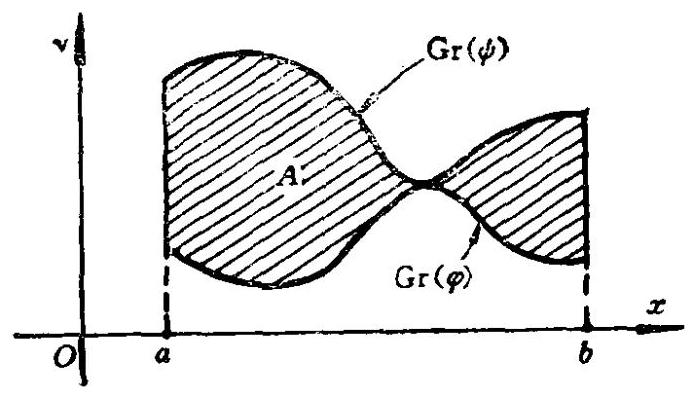
\includegraphics[max width=0.6\textwidth]{images/bo_d25ksc77aajc738obdgg_503_475_405_688_395_0.jpg}
\end{center}
\hspace*{3em} 

图 10-7

定理 ${10} \cdot  2 \cdot  4$ 设 $A$ 是度量空间(X, d)的任一非空集合,则

1) $A$ 是开集, $\overline{A\text{ 是闭集; }}$

2) $\partial A$ 是闭集,并且 $\partial A = \bar{A} \cap  \left( \overline{X - A}\right)$ .

证明 1 ) 由开集及 $A$ 的定义知 $A$ 是 $X$ 的开集,为了证明 $A$ 是闭集,我们证明 $X - \bar{A}$ 是开集.

首先不难证明下述结论成立:
$$x \in  \bar{A} \Leftrightarrow  \forall U \in  \mathcal{N}\left( x\right) ,U \cap  A \neq  \varnothing .$$
(*)

现任取 $x \in  X - \bar{A}$ . 由于 $x \in  \bar{A}$ ,故存在 $U \in  \mathcal{N}\left( x\right)$ 使得 $U \cap  A = \varnothing$ . 下面证明 $U \subset  X - \bar{A}$ .

事实上, $\forall y \in  U,U \in  \mathcal{N}\left( y\right)$ . 由于 $U \cap  A = \varnothing$ ,故 $y \in  \bar{A}$ ,从而 $y \in  X - \bar{A}$ 即 $U \subset  X - \bar{A}$ ,由 $x \in  X - \bar{A}$ 的任意性推知 $X - \bar{A}$ 是 $X$ 的开集,于是 $\bar{A}$ 是 $X$ 的闭集.

2) 由 $\partial A$ 的定义
$$\partial A = \{ x \in  X \mid  \forall U \in  \mathcal{N}\left( x\right) ,U \cap  A \neq  \varnothing ,U \cap  \left( {X - A}\right)  \neq  \varnothing \} .$$

故由上述 $\left( *\right)$ 式即知 $\partial A = \bar{A} \cap  \left( \overline{X - A}\right)$ . 由于 $\bar{A}$ 与 $\left( \overline{X - A}\right)$ 都是闭集,所以 $\partial A$ 是 $X$ 的闭集.

例6 $\forall a \in  \left( {X,d}\right) ,\forall \delta  \geq  0,S\left( {a,\delta }\right)$ 是闭集. 因为
$$S\left( {a,\delta }\right)  = \widehat{O}\bar{B}\left( {a,\delta }\right) .$$

\section*{4. 度量空间的子空间}

设(X, d)是任一度量空间, $Y \subset  X$ 是任一非空集合,我们用 $d$ . 表示 $d$ 在 $Y \times  Y$ 上的限制,直接由度量的定义可知, ${d}_{Y}$ 是 $Y$ 上的一个度量. 于是 $\left( {Y,{d}_{Y}}\right)$ 形成一个度量空间.

定义 度量空间 $\left( {Y,{d}_{Y}}\right)$ 称为度量空间(X, d)的子空间.

下面我们来研究度量空间(X, d)与子空间 $\left( {Y,{d}_{Y}}\right)$ 的开集之间的关系.

首先我们证明下述引理.

引理 若 $\left( {Y,{d}_{Y}}\right)$ 是(X, d)的子空间,则
$$\forall x \in  Y,\;\forall \delta  \geq  0,{B}_{{d}_{\Gamma }}\left( {x,\delta }\right)  = {B}_{d}\left( {x,\delta }\right)  \cap  Y.$$

证明 这可由 ${d}_{r}$ 的定义直接推出:
\begin{align*}
	&{B}_{{d}_{Y}}\left( {x,\delta }\right)  = \left\{  {y \in  Y \mid  {d}_{Y}\left( {y,x}\right)  < \delta }\right\}\\
	&= \{ y \in  Y \mid  d\left( {y,x}\right)  < \delta \}\\
	&= {B}_{d}\left( {x,\delta }\right)  \cap  Y\text{ . }
\end{align*}

\begin{center}
	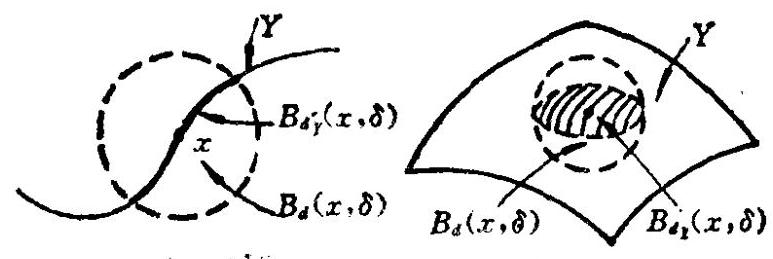
\includegraphics[max width=0.6\textwidth]{images/bo_d25ksc77aajc738obdgg_504_324_1281_773_259_0.jpg}
\end{center}
\hspace*{3em} 

图 10-8

定理 ${10} \cdot  2 \cdot  5\;A \subset  Y$ 是 $Y$ 的开集,当且仅当存在 $X$ 中的开集 $U$ 使得 $A = U \cap  Y$ .

证明 设 $A \subset  Y$ 是 $Y$ 的开集,则
\begin{align*}
	&\forall x \in  A,\exists {\delta }_{x} > 0 \Rightarrow  {B}_{{d}_{Y}}\left( {x,{\delta }_{x}}\right)  \subset  A\\
	&\Rightarrow  A = \mathop{\bigcup }\limits_{{x \in  A}}{B}_{{d}_{Y}}\left( {x,{\delta }_{x}}\right) ,
\end{align*}

令 $U = \mathop{\bigcup }\limits_{{x \in  A}}{E}_{d}\left( {x,{\delta }_{i}}\right)$ ,由定理 ${10} \cdot  2 \cdot  2$ 知 $U$ 是 $X$ 的开集,由引理 ${B}_{{d}_{Y}}\left( {x,{\delta }_{x}}\right)  = {B}_{d}\left( {x,{\delta }_{x}}\right)  \cap  Y$ ,故
\begin{align*}
	&A = \mathop{\bigcup }\limits_{{x \in  A}}{B}_{{d}_{Y}}\left( {x,{\delta }_{x}}\right)  = \mathop{\bigcup }\limits_{{x \in  A}}\left( {{B}_{d}\left( {x,{\delta }_{x}}\right)  \cap  Y}\right)\\
	&= \left( {\mathop{\bigcup }\limits_{{x \in  A}}{B}_{d}\left( {x,{\delta }_{x}}\right) }\right)  \cap  Y = U \cap  Y.
\end{align*}

反之,设存在 $X$ 中的开集 $U$ 使得 $A = U \cap  Y$ . 那末 $\forall x \in  A$ ,存在 ${\delta }_{x} > 0$ 使得 ${B}_{d}\left( {x,{\delta }_{x}}\right)  \subset  U$ ,再由 $\left. B\right| \;$ 理 ${B}_{d}\left( {x,{\delta }_{x}}\right)  = {B}_{d}\left( {x,{\delta }_{x}}\right)  \cap  Y$ 推得
\begin{align*}
	&A = \left( {\mathop{\bigcup }\limits_{{x \in  A}}{B}_{d}\left( {x,{\delta }_{x}}\right) }\right)  \cap  Y = \mathop{\bigcup }\limits_{{x \in  A}}\left( {{B}_{d}\left( {x,{\delta }_{x}}\right)  \cap  Y}\right)\\
	&= \mathop{\bigcup }\limits_{{x \in  A}}{B}_{{d}_{Y}}\left( {x,{\delta }_{x}}\right) .
\end{align*}

因此 $A$ 是 $Y$ 中的开集.

推论 若 $A \subset  Y$ 是 $X$ 的开集,则 $A$ 也是 $Y$ 的开集.

证明 因为 $A = A \cap  Y$ .

此推论的逆不成立,即 $Y$ 的开集不一定是 $X$ 的开集.

例7 考虑实数空间 $\left( {\mathbf{R},\left| \cdot \right| }\right)$ 的子空间 $\left( {\left\lbrack  {0,1}\right\rbrack  ,{\left| \cdot \right| }_{\left\lbrack  0,1\right\rbrack  }}\right)$ . $\forall a,b \in  \left\lbrack  {0,1}\right\rbrack$ 且 $a < b$ ,下述各集合
$$\text{ ] }a,b\left\lbrack  {,\left\lbrack  {0,b\left\lbrack  ,\right\rbrack  a,1}\right\rbrack  ,\phi ,\left\lbrack  {0,1}\right\rbrack  }\right\rbrack$$

都是 $\left\lbrack  {0,1}\right\rbrack$ 的开集,但 $\left\lbrack  {0,b\left\lbrack  ,\right\rbrack  a,1}\right\rbrack  ,\left\lbrack  {0,1}\right\rbrack$ 不是 $\mathbf{R}$ 的开集(这里 $b \neq  0,a \neq  1)$ ,而 $\rbrack a,b\lbrack$ 仍是 $\mathbf{R}$ 中的开集

例 8 考虑度量空间 $\left( {{\mathbf{R}}^{n},{d}_{1}}\right) \left( {n > 1}\right)$ ,令
$$H = \left\{  {\left( {{x}_{1},{x}_{2},\cdots ,{x}_{n}}\right)  \in  {\mathbf{R}}^{n} \mid  {x}_{n} \geq  0}\right\}  ,$$

则 $\left( {H,{d}_{1H}}\right)$ 是 $\left( {{\mathbf{R}}^{n},{d}_{1}}\right)$ 的子空间. 设 $A,B,C$ 是 $\left( {H,{d}_{1H}}\right)$ 中如下图所示的三个集合

显然 $A$ 是 $H$ 的开集,也是 ${\mathbf{R}}^{n}$ 的开集,因为 $A = {B}_{{d}_{1}}\left( {a,r}\right)  \subset  H$ ；

\begin{center}
	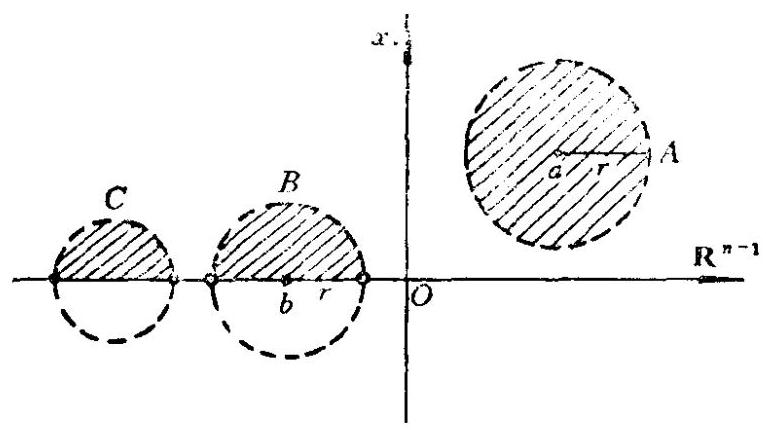
\includegraphics[max width=0.6\textwidth]{images/bo_d25ksc77aajc738obdgg_506_341_276_766_430_0.jpg}
\end{center}
\hspace*{3em} 

图 10-9

$B$ 是 $H$ 的开集,因为 $B = {B}_{{d}_{1}}\left( {b,r}\right)  \cap  H$ ,但 $B$ 不是 ${\mathrm{R}}^{n}$ 的开集； $C$ 不是 $H$ 的开集,当然也不是 ${\mathbf{R}}^{n}$ 的开集.

定理 ${10} \cdot  2 \cdot  6 : A \subset  Y$ 是 $Y$ 的闭集,当且仅当存在 $X$ 中的闭集 $V$ 使得 $A = V \cap  Y$ .

证明 设 $A \subset  Y$ 是 $Y$ 的闭集. 那末 $Y - A$ 是 $Y$ 的开集,从而由定理 ${10} \cdot  2 \cdot  5$ 知存在 $X$ 中的开集 $U$ 使得 $Y - A = U \cap  Y$ ,于是
\begin{align*}
	&A = Y - \left( {Y - A}\right)  = Y - \left( {U \cap  Y}\right)  = Y - U = \left( {X - U}\right)  \cap  Y\\
	&= V \cap  Y,
\end{align*}

这里 $V = X - U$ 是 $X$ 中的闭集.

反之设 $A = V \cap  Y$ ,这里 $V$ 是 $X$ 的闭集. 那末 $X - V$ 是 $X$ 的开集,从而由定理 ${10} \cdot  2 \cdot  5$ 知, $\left( {X - V}\right)  \cap  Y$ 是 $Y$ 的开集,而
$$\left( {X - V}\right)  \cap  Y = X \cap  Y - V \cap  Y = Y - A,$$

故 $A$ 是 $Y$ 的闭集.

推论 若 $A \subset  Y$ 是 $X$ 的闭集,则 $A$ 也是 $Y$ 的闭集.

证明 因为 $A = A \cap  Y$ .

注意,此推论的逆也是不成立的,即 $Y$ 的闭集不一定是 $X$ 的闭集.

\section*{习 题}

1. 设(X, d)是任一度量空间, $a \in  X$ . 证明:

1) $\forall {U}_{i} \in  \mathcal{N}\left( a\right) \left( {i = 1,2,\cdots ,n}\right) ,\mathop{\bigcap }\limits_{{i = 1}}^{n}{U}_{i} \in  \mathcal{N}\left( a\right)$ ,

2) $\mathop{\bigcap }\limits_{{U \in  \mathcal{X}\left( a\right) }}U = \{ a\}$ .

2. 设(X, d)是任一度量空间, $a \in  X$ . $\mathcal{B}$ 是 $\mathcal{N}\left( a\right)$ 的一子集,我们称 $\mathcal{B}$ 是 $a$ 的一个邻域基,如果
$$\forall U \in  \mathcal{V}\left( a\right) ,\exists V \in  \mathcal{B}, \Rightarrow  V \subset  U.$$

证明:(X, d)的每一点 $a$ 都有一个可数下降的邻域基 $\mathcal{B} = \left\{  {{V}_{n} \in  \mathcal{N}\left( a\right)  \mid  {V}_{n + 1}}\right.$  $\subset  {V}_{n},n \in  \mathbf{N}\}$ .

3. 设(X, d)是任一度量空间, $A \subset  X$ 是任一非空集合, $a \in  X$ .

1)证明:若 $a$ 是 $A$ 的聚点,则 $a$ 是 $A$ 的闭包点,反之则不然.

2) 设 $\mathcal{B}$ 是 $a$ 的一邻域基。证明:

$a$ 是 $A$ 的闭包点 $\Leftrightarrow  \forall V \in  \mathcal{B},V \cap  A \neq  \varnothing$ ,

$a$ 是 $A$ 的聚点 $\Leftrightarrow  \forall V \in  \mathcal{B},V \cap  \left( {A-\{ a\} }\right)  \neq  \varnothing$ .

3) 证明: $A$ 是 $X$ 的闭集,当且仅当 $A = \overline{{A}_{ \bullet  }}$

4) 证明: $\overline{\bar{A}} = \overline{{A}_{ \bullet  }}$

5) 证明: 若 $A \subset  B \subset  X$ ,则 $\bar{A} \subset  \bar{B}$ .

6) 证明: $\overline{A \cup  B} = \overline{A} \cup  \overline{B}$ . 举例说明 $\overline{A \cap  B} = \overline{A} \cap  \overline{B}$ 不成立.

4. 设(X, d)是任一度量空间, $A \subset  X$ 是任一非空集合.

1) 证明: $A$ 是 $X$ 的开集,当且仅当 $A = \overset{ \circ  }{A}$ .

2) 证明: $\overset{ \circ  }{A} = \overset{ \circ  }{{A}_{ \bullet  }}$

3) 证明: 若 $A \subset  B \subset  X$ ,则 $A \subset  B$ .

4) 证明: ${\left( A \cap  B\right) }^{ \circ  } = A \cap  B$ . 举例说明 ${\left( A \cup  B\right) }^{ \circ  } = A \cup  B$ 不成立.

5. 设(X, d)是任一度量空间, $A \subset  X$ 是任一非空集合. 证明:

1) $\partial A = A - A$ ,由此推得 $\partial A$ 是 $X$ 的闭集.

2) $\partial \overline{A} \subset  \partial A,\partial \overline{A} \subset  \partial A,\partial \left( {A \cup  B}\right)  \subset  \partial A \cup  \partial B$ .

3) 若 $\bar{A} \cap  \bar{B} = \varnothing$ ,则 $\partial \left( {A \cup  B}\right)  = \partial A \cup  \partial B$ .

4) $A$ 是开集当且仅当 $\partial A = \bar{A} - A$ .

6. 设(X, d)是任一度量空间, $E,F \subset  X$ 是两个不相交的闭集. 证明:

1) $\forall x \in  E,d\left( {x,F}\right)  = \mathop{\inf }\limits_{{y \in  F}}d\left( {x,y}\right)  > 0.\;\left( {d\left( {x,F}\right) \text{ 称为 }x\text{ 与 }F\text{ 的距离 }}\right)$

2) 存在两个开集 $U$ 与 $V$ 使得 $E \subset  U,F \subset  V$ 并且 $U \cap  V = \varnothing$ .

7. 设(X, d)是任一度量空间, $Y \subset  X$ 是一非空集合. 证明: 若 $A \subset  Y$ 是 $Y$ 的开(闭)集, $Y$ 是 $X$ 的开(闭)集. 则 $A$ 是 $X$ 的开(闭)集.

1. 写出图 10-9 中集合 $A$ 、 $B$ 、 $C$ 分别在 $\left( {{\mathbf{R}}^{2},{d}_{1}}\right)$ 与 $\left( {\mathbf{H},{d}_{1H}}\right)$ 中的 [ ] 包、内部与边界.

9. 设 $\mathcal{F}$ 是如下定义的 $\mathrm{R}$ 的子-集族:

$\mathcal{F} = \{ U \subset  \mathrm{R} \mid  U = \bigodot$ 或 $\mathrm{R} - U$ 是可数集 $\} .$

1 )证明: $\mathcal{F}$ 是 $\mathrm{R}$ 的一个拓扑.

2) 证明: 若 ${U}_{n} \in  \mathcal{F},\left( {n \in  \mathbf{N}}\right)$ ,则 $\mathop{\bigcap }\limits_{{n = 1}}^{{+\infty }}{U}_{n} \in  \mathcal{F}$ .

3) 证明: $\mathcal{F}$ 不具有Hausdorff分离性,即 “ $\forall x,y \in  \mathbf{R}$ 且 $x \neq  y$ ,存在 $U$ , $V \in  \mathcal{F}$ 使得 $x \in  U,y \in  V$ 且 $U \cap  V =  \oslash$ ”不成立.

4) 若改 $\mathcal{F}$ 为 ${\mathcal{F}}^{\prime }$ :
$${\mathcal{F}}^{\prime } = \{ U \subset  R \mid  U = \varnothing \text{ 或 }R - U\text{ 为有限集 }\} .$$

试问上述 1) 、2) 、3) 的结论仍然成立吗?

\section{度量空间的点序列极限, 映射的极限与连续性}

\section*{1. 度量空间的点序列极限}

定义 设 $X$ 是任一非空集合. 从 $\mathbf{N}$ 到 $X$ 的任一映射 $x : \mathbf{N} \rightarrow  X$ 称为 $X$ 的一个点序列,简记为 $\left\langle  {x}_{n}\right\rangle  .{x}_{n}\left( {n \in  \mathbf{N}}\right)$ 称为此序列的第 $n$ 项或通项.

例 1 设 $\left\langle  {x}_{ni}\right\rangle  \left( {i = 1,2,\cdots ,k}\right)$ 是 $k$ 个实数序列,令

${x}_{n} = \left( {{x}_{n1},{x}_{n2},\cdots ,{x}_{nk}}\right) \left( {\forall n \in  \mathbf{N}}\right)$ ,则 $\left\langle  {x}_{n}\right\rangle$ 是 ${\mathbf{R}}^{k}$ 的一个点序列.

例 2 设 $\left\langle  {x}_{n}\right\rangle$ 与 $\left\langle  {y}_{n}\right\rangle$ 是两个实数序列,令
$${z}_{n} = {x}_{n} + i{y}_{n}\left( {\forall n \in  \mathbf{N}}\right) ,$$

则 $\left\langle  {z}_{n}\right\rangle$ 是 $\mathrm{C}$ 的一个复数序列.

例 3 设 ${f}_{n} \in  {C}^{0}\left( {\left\lbrack  {a,b}\right\rbrack  ,\mathbb{R}}\right) \left( {\forall n \in  \mathbf{N}}\right)$ ,则 $\left\langle  {f}_{n}\right\rangle$ 是 ${C}^{0}(\left\lbrack  {a,b}\right\rbrack$ , R)的一个连续函数序列.

定义 设(X, d)是任一度量空间, $\left\langle  {x}_{n}\right\rangle$ 是 $X$ 的任一点序列.

1) 我们称 $\left\langle  {x}_{n}\right\rangle$ 收敛,如果存在 $x \in  X$ ,它具有下述性质:
$$\left( {\forall \varepsilon  > 0}\right) \left( {\exists N \in  \mathbf{N}}\right) \left( {\forall n \in  \mathbf{N},n \geq  N}\right)  \Rightarrow  d\left( {{x}_{n},x}\right)  < \varepsilon .$$

这时我们也称点序列 $\left\langle  {x}_{n}\right\rangle$ 当 $n \rightarrow   + \infty$ 时收敛于 $x$ 或以 $x$ 为极限,记为
$$\mathop{\lim }\limits_{{n \rightarrow   + \infty }}{x}_{n} = x\text{ 或 }{x}_{n} \rightarrow  x\left( {n \rightarrow   + \infty }\right) .$$

2) 我们称 $\left\langle  {x}_{n}\right\rangle$ 发散,如果 $\left\langle  {x}_{n}\right\rangle$ 不收敛.

下面我们对度量空间点序列的收敛性作两点说明.

第一: 由度量空间(X, d)的Hausdorff分离性推知,若 $X$ 的点序列 $\left\langle  {x}_{n}\right\rangle$ 有极限 $x$ ,则此极限是唯一的.

第二: 点序列 $\left\langle  {x}_{n}\right\rangle$ 的收敛性是依赖于 $X$ 上所选择的度量 $d$ 的. 也就是说, $X$ 的同一点序列 $\left\langle  {x}_{n}\right\rangle$ 对度量 ${d}_{1}$ 收敛,但对度量 ${d}_{2}$ 可能发散。

然而若 ${d}_{1},{d}_{2}$ 是 $X$ 上的两个等价度量,则
$$\mathop{\lim }\limits_{{n \rightarrow   + \infty }}{x}_{n} = {}^{\frac{{d}_{1}}{}}x\text{ 当且仅当 }\mathop{\lim }\limits_{{n \rightarrow   + \infty }}{x}_{n} = {}^{\frac{{d}_{2}}{}}x.$$

事实上,由于 ${d}_{1}$ 与 ${d}_{2}$ 等价,故存在常数 $A > 0,B > 0$ 使得
$$A{d}_{1}\left( {x,y}\right)  \leq  {d}_{2}\left( {x,y}\right)  \leq  B{d}_{1}\left( {x,y}\right) ,\;\forall x,y \in  X.$$

从而
$$A{d}_{1}\left( {{x}_{n},x}\right)  \leq  {d}_{2}\left( {{x}_{n},x}\right)  \leq  B{d}_{1}\left( {{x}_{n},x}\right) \left( {\forall n \in  \mathbf{N}}\right) .$$

由此即可推得我们的结论.

特别地,当 $X = {\mathbf{R}}^{k}$ 时,由于 ${\mathbf{R}}^{k}$ 上的三个基本度量 ${d}_{1},{d}_{2},{d}_{3}$ 互相等价,因此在 ${\mathbf{R}}^{k}$ 中考虑它的点序列的极限时,我们可以取这三个度量中的任何一个而不会影响点序列的收敛性.

现在我们来研究 ${\mathbf{R}}^{k}$ 的点序列与 $\mathbf{C}$ 的复数序列的收敛性.

定理 ${10} \cdot  3 \cdot  1$ 设 $\left\langle  {x}_{n}\right\rangle$ 是 ${\mathrm{R}}^{k}\left( {k > 1}\right)$ 中的任一点序列, $x \in  {\mathrm{R}}^{k}$ . 令
$${x}_{n} = \left( {{x}_{n1},{x}_{n2},\cdots ,{x}_{nk}}\right) \left( {n \in  \mathbf{N}}\right) ,x = \left( {{\xi }_{1},{\xi }_{2},\cdots {\xi }_{k}}\right) ,$$

则
$$\mathop{\lim }\limits_{{n \rightarrow   + \infty }}{x}_{n} = x \Leftrightarrow  \mathop{\lim }\limits_{{n \rightarrow   + \infty }}{x}_{ni} = {\xi }_{i}\left( {i = 1,2,\cdots ,k}\right) .$$

证明 在 ${\mathbf{R}}^{k}$ 中取基本度量 ${d}_{3}$ . 则
\begin{align*}
	&\mathop{\lim }\limits_{{n \rightarrow   + \infty }}{x}_{n}\overset{{d}_{3}}{ = }x \Leftrightarrow  \left( {\forall \varepsilon  > 0}\right) \left( {\exists N \in  \mathbf{N}}\right) \left( {\forall n \in  \mathbf{N},n \geq  N}\right)\\
	&\Rightarrow  {d}_{3}\left( {{x}_{n},x}\right)  < \varepsilon\\
	&\Leftrightarrow  \left( {\forall \varepsilon  > 0}\right) \left( {\exists N \in  \mathbf{N}}\right) \left( {\forall n \in  \mathbf{N},n \geq  N}\right)\\
	&\Rightarrow  \mathop{\max }\limits_{{1 \leq  i \leq  k}}\left| {{x}_{ni} - {\xi }_{i}}\right|  < \varepsilon\\
	&\Leftrightarrow  \left( {\forall \varepsilon  > 0}\right) \left( {\exists N \in  \mathbf{N}}\right) \left( {\forall n \in  \mathbf{N},n \geq  N}\right)\\
	&\Rightarrow  \left| {{x}_{ni} - {\xi }_{i}}\right|  < \varepsilon \left( {i = 1,2,\cdots ,k}\right)\\
	&\Leftrightarrow  \mathop{\lim }\limits_{{n \rightarrow   + \infty }}{x}_{ni} = {\xi }_{i}\left( {i = 1,2\cdots ,k}\right) \text{ . }
\end{align*}

此定理表明在 ${\mathbf{R}}^{k}$ 中求点序列 $\left\langle  {x}_{n}\right\rangle$ 的极限可化为求 $\left\langle  {x}_{n}\right\rangle$ 的各相应分量组成的实数序列 $\left\langle  {x}_{ni}\right\rangle  \left( {i = 1,2,\cdots ,k}\right)$ 的极限.

定理 ${10} \cdot  3 \cdot  2$ 设 $\left\langle  {z}_{n}\right\rangle   = \left\langle  {{x}_{n} + i{y}_{n}}\right\rangle$ 是 $\mathrm{C}$ 的任一复数序列, $z =$  $x + {iy} \in  \mathbf{C}$ ,则
$$\mathop{\lim }\limits_{{n \rightarrow   + \infty }}{z}_{n} = z \Leftrightarrow  \mathop{\lim }\limits_{{n \rightarrow   + \infty }}{x}_{n} = x,\mathop{\lim }\limits_{{n \rightarrow   + \infty }}{y}_{n} = y.$$

证明 根据复数模的定义,
\begin{align*}
	&\left| {{z}_{n} - z}\right|  = \left| {\left( {{x}_{n} - x}\right)  + i\left( {{y}_{n} - y}\right) }\right|\\
	&= \sqrt{{\left( {x}_{n} - x\right) }^{2} + {\left( {y}_{n} - y\right) }^{2}}\text{ . }
\end{align*}

由此立即推得
\begin{align*}
	&\mathop{\lim }\limits_{{n \rightarrow   + \infty }}{z}_{n} = z \Leftrightarrow  \mathop{\lim }\limits_{{n \rightarrow   + \infty }}\left| {{z}_{n} - z}\right|  = 0\\
	&\Leftrightarrow  \mathop{\lim }\limits_{{n \rightarrow   + \infty }}\left( {{x}_{n} - x}\right)  = 0,\mathop{\lim }\limits_{{n \rightarrow   + \infty }}\left( {{y}_{n} - y}\right)  = 0\\
	&\Leftrightarrow  \mathop{\lim }\limits_{{n \rightarrow   + \infty }}{x}_{n} = x,\mathop{\lim }\limits_{{n \rightarrow   + \infty }}{y}_{n} = y.
\end{align*}

这个定理表明求复数序列 $\left\langle  {z}_{n}\right\rangle$ 的极限可化 为分别求 ${z}_{n}(n \in$ N)的实部与虚部系数组成的实数序列 $\left\langle  {x}_{n}\right\rangle$ 与 $\left\langle  {y}_{n}\right\rangle$ 的极限.

附注 关于例 3 中 ${C}^{0}\left( {\left\lbrack  {a,b}\right\rbrack  ,\mathbf{R}}\right)$ 的连续函数序列 $\left\langle  {f}_{n}\right\rangle$ 的收敛性, 也是相对它的某一个度量而言的.

例如在 ${C}^{0}\left( {\left\lbrack  {a,b}\right\rbrack  ,\mathbf{R}}\right)$ 中取由它的一致收敛范数 $\parallel  \cdot  {\parallel }_{\infty }$ 所诱导的度量 $d$ (称为一致度量),即
$$\forall f,g \in  {C}^{0}\left( {\left\lbrack  {a,b}\right\rbrack  ,\mathbf{R}}\right) ,d\left( {f,g}\right)  = \parallel f - g\parallel \ldots$$

若 $f,{f}_{n} \in  {C}^{0}\left( {\left\lbrack  {a,b}\right\rbrack  ,\mathbf{R}}\right) \left( {n \in  \mathbf{N}}\right)$ ,则序列 $\left\langle  {f}_{n}\right\rangle$ 关于此度量 $d$ 收敛于 $f$ 也称为 $\left\langle  {f}_{n}\right\rangle$ 在 $\left\lbrack  {a,b}\right\rbrack$ 上一致收敛于 $f$ .

关于函数序列的一致收敛性问题, 我们将在第 12 章中进行专门研究.

作为点序列极限的应用, 我们来证明下述定理.

定理 ${10} \cdot  3 \cdot  3$ 设(X, d)是任一度量空间,则 $A \subset  X$ 是闭集的充分必要条件是:

若 ${x}_{n} \in  A\left( {n \in  \mathbf{N}}\right)$ 且 ${x}_{n} \rightarrow  x\left( {n \rightarrow   + \infty }\right)$ ,则 $x \in  A$ .

证明 必要性 设 $A \subset  X$ 是闭集, ${x}_{n} \in  A\left( {n \in  \mathbf{N}}\right)$ 并且 ${x}_{n} \rightarrow  x$  $\left( {n \rightarrow   + \infty }\right)$ . 我们证明 $x \in  A$ .

用反证法. 假设 $x \in  A$ ,则 $x \in  X - A$ : 由于 $X - A$ 是开集,故存在 $\delta  > 0$ 使得 $B\left( {x,\delta }\right)  \subset  X - A$ . 因为 ${x}_{n} \rightarrow  x\left( {n \rightarrow   + \infty }\right)$ ,故存在 $N$  $\in  \mathbf{N}$ 使得
$$\forall n \in  \mathbf{N},n \geq  N,{x}_{n} \in  B\left( {x,\delta }\right)  \Rightarrow  {x}_{n} \in  X - A.$$

这与 ${x}_{n} \in  A\left( {n \in  \mathbf{N}}\right)$ 矛盾. 因此 $x \in  A$ .

充分性 设定理的条件成立,我们来证明 $A$ 是闭集.

为此只需证明 $X - A$ 是开集. 仍然 用反证法. 假设 $X - A$ 不是开集. 于是由开集定义知
\begin{align*}
	&\left( {\exists {x}_{0} \in  X - A}\right) \left( {\forall n \in  \mathbf{N}}\right) \left( {\exists {x}_{n} \in  B\left( {{x}_{0},\frac{1}{n}}\right) }\right)\\
	&\Rightarrow  {x}_{n} \in  X - A\text{ . }
\end{align*}

由此得到 $X$ 的一点序列 $\left\langle  {x}_{n}\right\rangle$ 使得
$${x}_{n} \in  A\left( {n \in  \mathbf{N}}\right) ,{x}_{n} \rightarrow  {x}_{0}\left( {n \rightarrow   + \infty }\right) .$$

由已知条件知, ${x}_{0} \in  A$ ,这与 ${x}_{0} \in  X - A$ 矛盾,因此 $X - A$ 为开集, 即 $A$ 为闭集.

此定理是用序列的极限来刻划度量空间的闭集的, 应用它去判断集合的闭性十分方便.

例 4 利用上述定理证明: 对任意集合 $A \subset  X$ , $\bar{A}$ 是闭集.

事实上,若 $A = \varnothing$ ,则 $\bar{A} = \varnothing$ 为闭集. 若 $A = \varnothing$ ,则任取 $\bar{A}$ 中的点序列 $\left\langle  {x}_{n}\right\rangle$ 使得 ${x}_{n} \rightarrow  x\left( {n \rightarrow   + \infty }\right)$ ,我们来证明 $x \in  \overrightarrow{A}$ .

若存在 ${n}_{0} \in  \mathbf{N}$ 使得 ${x}_{{n}_{0}} = x$ ,则 $x \in  \bar{A}$ ,因此不妨设 $\forall n \in  \mathbf{N}$ , ${x}_{n} = x$ . 由于 $\forall n \in  \mathbf{N},{x}_{n} \in  A$ ,故存在 ${y}_{n} \in  A$ 使得 $d\left( {{x}_{n},{y}_{n}}\right)  <$  $\frac{1}{n},{y}_{n} \neq  x$ . 由此得到 $A$ 的点序列 $\left\langle  {y}_{n}\right\rangle$ . 由不等式
$$d\left( {{y}_{n},x}\right)  \leq  d\left( {{y}_{n},{x}_{n}}\right)  + d\left( {{x}_{n},x}\right)  < \frac{1}{n} + d\left( {{x}_{n},x}\right)$$

知, ${y}_{n} \rightarrow  x\left( {n \rightarrow   + \infty }\right)$ .

现任取 $U \in  \mathcal{N}\left( x\right)$ . 于是存在 $n \in  \mathbf{N}$ 使得
$${y}_{n} \in  U \cap  \left( {A-\{ x\} }\right) .$$

此即表明 $x \in  \overline{A}$ ,因此 $\overline{A}$ 是闭集.

\section*{2. 度量空间上的映射的极限与连续性}

定义 设(X, d)与(Y, D)是两个度量空间, $A \subset  X$ 是任一非空集合, $f : A \rightarrow  Y$ 是任一映射. $a \in  X,l \in  Y$ .

1)我们称映射 $f$ 当 $x$ 趋于 $a$ 时以 $l$ 为极限,如果 $a$ 是 $A$ 的聚点, 并且下述性质成立:
\begin{align*}
	&\left( {\forall \varepsilon  > 0}\right) \left( {\exists \delta  > 0}\right) \left( {\forall x \in  A,0 < d\left( {a,x}\right)  < \delta }\right)\\
	&\Rightarrow  D\left( {f\left( x\right) ,l}\right)  < \varepsilon .
\end{align*}

这时记为
$$\mathop{\lim }\limits_{{x \rightarrow  a}}f\left( x\right)  = l\text{ 或 }f\left( x\right)  \rightarrow  l\left( {x \rightarrow  a}\right) .$$

2) 我们称映射 $f$ 在 $a$ 处连续,如果 $a \in  A$ 并且下述性质成立:
\begin{align*}
	&\left( {\forall \varepsilon  > 0}\right) \left( {\exists \delta  > 0}\right) \left( {\forall x \in  A,d\left( {a,x}\right)  < \delta }\right)\\
	&\Rightarrow  D\left( {f\left( x\right) ,f\left( a\right) }\right)  < \varepsilon .
\end{align*}

3) 我们称映射 $f$ 在 $A$ 上连续,如果 $f$ 在 $A$ 的每一点 $x$ 处连续.

附注 1) 由上述定义可知,当 $X = Y = \mathbf{R}$ ,并且 $d\left( {x,y}\right)  =$  $D\left( {x,y}\right)  = \left| {x - y}\right|$ 时,上面的定义就是我们在第 4 章中研究过的一元实值函数的极限与连续性定义.

2) 现在设 ${d}^{\prime }$ 是 $X$ 上的另一度量, ${D}^{\prime }$ 是 $Y$ 上的另一度量,并且 ${d}^{\prime }$ 与 $d$ 等价, ${D}^{\prime }$ 与 $D$ 等价. 则容易验证
$$\mathop{\lim }\limits_{{x \rightarrow  a}}f{\left( x\right) }^{d}\overset{d,D}{ = }l\text{ 当且仅当 }\mathop{\lim }\limits_{{x \rightarrow  a}}f\left( x\right) \overset{{d}^{\prime },{D}^{\prime }}{ = }l.$$

换句话说,映射 $f : A\left( { \subset  X}\right)  \rightarrow  Y$ 的极限与连续性定义跟 $X$ 中的等价度量及 $Y$ 中的等价度量的选择无关.

因此,特别地,若我们考虑映射 $f : A\left( { \subset  {\mathbf{R}}^{k}}\right)  \rightarrow  {\mathbf{R}}^{m}$ ,则可以在 ${\mathbf{R}}^{k}$ 与 ${\mathbf{R}}^{m}$ 中任取各自的基本度量而不影响 $f$ 的极限存在与连续性.

下面我们列出两类常用映射的极限与连续性定义, 以加深印象. 1) $k$ 元实值函数的极限与连续性定义

取 $X = {\mathbf{R}}^{k}\left( {k \geq  1}\right) ,d$ 为 ${\mathbf{R}}^{k}$ 中任一基本度量,如 ${d}_{1}$ ;

$Y = \mathbf{R},D$ 为 $\mathbf{R}$ 上的绝对值度量 $\left| \cdot \right|$ ;
$$x = \left( {{x}_{1},{x}_{2},\cdots ,{x}_{k}}\right) ,a = \left( {{a}_{1},{a}_{2},\cdots ,{a}_{k}}\right)  \in  {\mathbf{R}}^{k},$$

则映射 $f : A\left( { \subset  {\mathrm{R}}^{k}}\right)  \rightarrow  \mathrm{R}$ 称为 $k$ 元实值函数,这时

1) 映射 $f : A\left( { \subset  {\mathbf{R}}^{k}}\right)  \rightarrow  \mathbf{R}$ 当 $x \rightarrow  a$ 时以 $l$ 为极限,当且仅当
\begin{align*}
	&\left( {\forall \varepsilon  > 0}\right) \left( {\exists \delta  > 0}\right) \left( {\forall x \in  A,0 < \sqrt{\mathop{\sum }\limits_{{i = 1}}^{k}{\left( {x}_{i} - {a}_{i}\right) }^{2}} < \delta }\right)\\
	&\Rightarrow  \left| {f\left( x\right)  - l}\right|  < \varepsilon \text{ . }
\end{align*}

2) 映射 $f : A\left( { \subset  {\mathbf{R}}^{k}}\right)  \rightarrow  \mathbf{R}$ 在 $a$ 处连续,当且仅当
\begin{align*}
	&\left( {\forall \varepsilon  > 0}\right) \left( {\exists \delta  > 0}\right) \left( {\forall x \in  A,\sqrt{\mathop{\sum }\limits_{{i = 1}}^{k}{\left( {x}_{i} - {a}_{i}\right) }^{2}} < \delta }\right)\\
	&\Rightarrow  \left| {f\left( x\right)  - f\left( a\right) }\right|  < \varepsilon \text{ . }
\end{align*}

例 5 证明: 二元函数 $f : {\mathbb{R}}^{2} \rightarrow  \mathbb{R}$
$$f\left( {x,y}\right)  = \left\{  \begin{array}{ll} \frac{{x}^{2}y}{{x}^{2} + {y}^{2}}, & \text{ 若 }\left( {x,y}\right)  > \left( {0,0}\right) \\  0, & \text{ 若 }\left( {x,y}\right)  = \left( {0,0}\right)  \end{array}\right.$$

在(0,0)处连续.

事实上, $\forall \left( {x,y}\right)  \neq  \left( {0,0}\right)$ ,我们有
$$\left| {f\left( {x,y}\right)  - f\left( {0,0}\right) }\right|  = \left| \frac{{x}^{2}y}{{x}^{2} + {y}^{2}}\right|  \leq  \left| y\right|  \leq  \sqrt{{x}^{2} + {y}^{2}}.$$

若在 ${\mathbf{R}}^{2}$ 中取基本度量 ${d}_{1}$ ,则
\begin{align*}
	&\left( {\forall \varepsilon  > 0}\right) \left( {\exists \delta  = \varepsilon  > 0}\right) \left( {\forall \left( {x,y}\right)  \in  {\mathbf{R}}^{2},0 < \sqrt{{\left( x - 0\right) }^{2} + {\left( y - 0\right) }^{2}} < \delta }\right)\\
	&\Rightarrow  \left| {f\left( {x,y}\right) -\int \left( {0,0}\right) }\right|  < \varepsilon .
\end{align*}

因此 $\mathop{\lim }\limits_{{\left( {x,y}\right)  \rightarrow  \left( {0,0}\right) }}f\left( {x,y}\right)  = f\left( {0,0}\right)$ ,从而 $f$ 在(0,0)处连续.

例6 设二元函数 $f : {\mathbf{R}}^{2} \rightarrow  \mathbf{R}$ 定义如下:
$$f\left( {x,y}\right)  = \left\{  \begin{array}{ll} \frac{xy}{{x}^{2} + {y}^{2}}, & \text{ 若 }\left( {x,y}\right)  \neq  \left( {0,0}\right) ; \\  0, & \text{ 若 }\left( {x,y}\right)  = \left( {0,0}\right) . \end{array}\right.$$

证明: $f$ 当 $\left( {x,y}\right)  \rightarrow  \left( {0,0}\right)$ 时极限不存在.

事实上,若令 $y = {kx}\left( {k \in  \mathbf{R}}\right)$ ,则 $\forall x \neq  0$ ,
$$f\left( {x,{kx}}\right)  = \frac{k{x}^{2}}{{x}^{2} + {k}^{2}{x}^{2}} = \frac{k}{1 + {k}^{2}}.$$

于是 $\mathop{\lim }\limits_{{x \rightarrow  0}}f\left( {x,{kx}}\right)  = \frac{k}{1 + {k}^{2}}$ . 此极限依赖于 $k$ ,故 $f$ 当 $\left( {x,y}\right)  \rightarrow  (0$ , 0 )时不可能有极限存在.

对于 $k$ 元实值函数的极限与连续性的运算性质. 可综合为下述定理.

定理 ${10} \cdot  3 \cdot  4$ 设 $f,g : A\left( { \subset  {\mathbf{R}}^{k}}\right)  \rightarrow  \mathbf{R}$ 是任意两个 $k$ 元实值函数,并且当 $x \rightarrow  a$ 时有极限存在,则 $f + g,{fg}$ 与 $\frac{f}{g} : A \rightarrow  \mathbf{R}$ 当 $x \rightarrow$  $a$ 时也有极限存在 $\left( {\text{ 对 }\frac{f}{g},\mathop{\lim }\limits_{{x \rightarrow  a}}g\left( x\right)  \neq  0}\right)$ ,并且
\begin{align*}
	&\mathop{\lim }\limits_{{x \rightarrow  a}}\left( {f + g}\right) \left( x\right)  = \mathop{\lim }\limits_{{x \rightarrow  a}}f\left( x\right)  + \mathop{\lim }\limits_{{x \rightarrow  a}}g\left( x\right) ,\\
	&\mathop{\lim }\limits_{{x \rightarrow  a}}\left( {fg}\right) \left( x\right)  = \mathop{\lim }\limits_{{x \rightarrow  a}}f\left( x\right)  \cdot  \mathop{\lim }\limits_{{x \rightarrow  a}}g\left( x\right) ,\\
	&\mathop{\lim }\limits_{{x \rightarrow  a}}\left( \frac{f}{g}\right) \left( x\right)  = \mathop{\lim }\limits_{{x \rightarrow  a}}f\left( x\right) /\mathop{\lim }\limits_{{x \rightarrow  a}}g\left( x\right) .
\end{align*}

此定理的证明留给读者作为练习.

例7 证明: 如下定义的映射 $\varphi  : \left\lbrack  {0, + \infty \left\lbrack  {\times \left\lbrack  {0,{2\pi }}\right\rbrack   \times  \left\lbrack  {0,\pi }\right\rbrack  }\right\rbrack  }\right.$  $\rightarrow  \mathrm{R} :$
\begin{align*}
	&\forall \left( {r,\theta ,\alpha }\right)  \in  \left\lbrack  {0, + \infty \left\lbrack  {\times \left\lbrack  {0,{2\pi }}\right\rbrack   \times  \left\lbrack  {0,\pi }\right\rbrack  ,\varphi \left( {r,\theta ,\alpha }\right) }\right\rbrack  }\right.\\
	&= r\sin \theta \cos \alpha
\end{align*}

在 $\lbrack 0, + \infty \left\lbrack  {\times \left\lbrack  {0,{2\pi }}\right\rbrack   \times  \left\lbrack  {0,\pi }\right\rbrack  }\right\rbrack$ 上连续.

为此我们可以令 ${\varphi }_{1},{\varphi }_{2},{\varphi }_{3} : \left\lbrack  {0, + \infty \left\lbrack  {\times \left\lbrack  {0,{2\pi }}\right\rbrack   \times  \left\lbrack  {0,\pi }\right\rbrack   \rightarrow  \mathbf{R}}\right\rbrack  }\right.$ 为:
\begin{align*}
	&\forall \left( {r,\theta ,\alpha }\right)  \in  \left\lbrack  {0, + \infty \left\lbrack  {\times \left\lbrack  {0,{2\pi }}\right\rbrack   \times  \left\lbrack  {0,\pi }\right\rbrack  ,{\varphi }_{1}\left( {r,\theta ,\alpha }\right) }\right\rbrack  }\right.\\
	&= r,{\varphi }_{2}\left( {r,\theta ,\alpha }\right)  = \sin \theta ,{\varphi }_{3}\left( {r,\theta ,\alpha }\right)  = \cos \alpha .
\end{align*}

显然 ${\varphi }_{1},{\varphi }_{2},{\varphi }_{3}$ 在 $\lbrack 0, + \infty \left\lbrack  {\times \left\lbrack  {0,{2\pi }}\right\rbrack   \times  \left\lbrack  {0,\pi }\right\rbrack  }\right\rbrack$ 上连续,于是根据上述定理知, $\varphi  = {\varphi }_{1} \cdot  {\varphi }_{2} \cdot  {\varphi }_{3}$ 在 $\lbrack 0, + \infty \left\lbrack  {\times \left\lbrack  {0,{2\pi }}\right\rbrack   \times  \left\lbrack  {0,\pi }\right\rbrack  }\right\rbrack$ 上连续. 例 8 计算 $\mathop{\lim }\limits_{{\left( {x,y}\right)  \rightarrow  \left( {0;0}\right) }}{\left( {x}^{2} + {y}^{2}\right) }^{{x}^{2}{y}^{2}}$ .

令 $f\left( {x,y}\right)  = {\left( {x}^{2} + {y}^{2}\right) }^{{x}^{2}{y}^{2}},\left( {x,y}\right)  = \left( {0,0}\right)$ . 两边取自然对数得
\begin{align*}
	&\log f\left( {x,y}\right)  = {x}^{2}{y}^{2}\log \left( {{x}^{2} + {y}^{2}}\right)\\
	&= \frac{{x}^{2}{y}^{2}}{{x}^{2} + {y}^{2}} \cdot  \left( {{x}^{2} + {y}^{2}}\right) \log \left( {{x}^{2} + {y}^{2}}\right) .
\end{align*}

由于
\begin{align*}
	&0 \leq  \frac{{x}^{2}{y}^{2}}{{x}^{2} + {y}^{2}} \leq  \frac{1}{2}\left| {xy}\right|  \leq  \frac{1}{4}\left( {{x}^{2} + {y}^{2}}\right) ,\\
	&\left( {{x}^{2} + {y}^{2}}\right) \log \left( {{x}^{2} + {y}^{2}}\right)  = z\log z\;\left( {z = {x}^{2} + {y}^{2}}\right) ,
\end{align*}

故
\begin{align*}
	&\mathop{\lim }\limits_{{\left( {x : y}\right)  \rightarrow  \left( {0 : 0}\right) }}\frac{{x}^{2}{y}^{2}}{{x}^{2} + {y}^{2}} = 0,\\
	&\mathop{\lim }\limits_{{\left( {x;y}\right)  \rightarrow  \left( {0;0}\right) }}\left( {{x}^{2} + {y}^{2}}\right) \log \left( {{x}^{2} + {y}^{2}}\right)  = \mathop{\lim }\limits_{{z \rightarrow  0}}z\log z = 0.
\end{align*}

因此由上述定理得到
\begin{align*}
	&\mathop{\lim }\limits_{{\left( {x;y}\right)  \rightarrow  \left( {0;0}\right) }}\log f\left( {x,y}\right)  = \mathop{\lim }\limits_{{\left( {x;y}\right)  \rightarrow  \left( {0;0}\right) }}\frac{{x}^{2}{y}_{2}}{{x}^{2} + {y}_{2}}\\
	&\times  \mathop{\lim }\limits_{{\left( {x;y}\right)  \rightarrow  \left( {0;0}\right) }}\left( {{x}^{2} + {y}^{2}}\right) \log \left( {{x}^{2} + {y}^{2}}\right)  = 0.
\end{align*}

由此推得
$$\mathop{\lim }\limits_{{\left( {x;y}\right)  \rightarrow  \left( {0;0}\right) }}{\left( {x}^{2} + {y}^{2}\right) }^{{x}^{2}{y}^{2}} = 1.$$

2) $k$ 元向量值函数的极限与连续性定义

取 $X = {\mathbf{R}}^{k}\left( {k \geq  1}\right)$ , $d$ 为 ${\mathbf{R}}^{k}$ 中的任一基本度量,如 ${d}_{2}$ ；

$Y = {\mathrm{R}}^{m}\left( {m > 1}\right) ,D$ 为 ${\mathrm{R}}^{m}$ 中的任一基本度量 ${d}_{3}$ ；
\begin{align*}
	&x = \left( {{x}_{1},{x}_{2},\cdots ,{x}_{k}}\right) ,a = \left( {{a}_{1},{a}_{2},\cdots ,{a}_{k}}\right)  \in  {\mathbf{R}}^{k};\\
	&l = \left( {{l}_{1},{l}_{2},\cdots ,{l}_{m}}\right) ,\\
	&f\left( x\right)  = \left( {{f}_{1}\left( x\right) ,{f}_{2}\left( x\right) ,\cdots ,{f}_{m}\left( x\right) }\right)  \in  {\mathbf{R}}^{m},
\end{align*}

则映射 $f : A\left( { \subset  {\mathbf{R}}^{k}}\right)  \rightarrow  {\mathbf{R}}^{m}$ 称为 $k$ 元向量值函数, $\forall i = 1,2,\cdots$ . $m$ . 映射 ${f}_{i} : A\left( { \subset  {\mathbf{R}}^{k}}\right)  \rightarrow  \mathbf{R}$ 称为 $f$ 的分量函数,它是 $k$ 元实值函数, 这时

1) 映射 $f : A\left( { \subset  {\mathbf{R}}^{k}}\right)  \rightarrow  {\mathbf{R}}^{m}$ 当 $x \rightarrow  a$ 时以 $l$ 为极限当且仅当
$$\left( {\forall \varepsilon  > 0}\right) \left( {\exists \delta  > 0}\right) \left( {\forall x \in  A,0 < \mathop{\sum }\limits_{{i = 1}}^{k}\left| {{x}_{i} - {a}_{i}}\right|  < \delta }\right)$$

$\Rightarrow  \mathop{\max }\limits_{{1 \leq  i < m}}\left| {{f}_{i}\left( x\right)  - {l}_{i}}\right|  < \varepsilon  \Leftrightarrow  \left| {{f}_{i}\left( x\right)  - {l}_{i}}\right|  < \varepsilon \left( {\forall i = 1,2,\cdots ,m}\right) .$

因此
$$\mathop{\lim }\limits_{{x \rightarrow  a}}f\left( x\right)  = l \Leftrightarrow  \mathop{\lim }\limits_{{x \rightarrow  a}}{f}_{i}\left( x\right)  = {l}_{i}\left( {i = 1,2,\cdots ,m}\right) .$$

2) 映射 $f : A\left( { \subset  {\mathbf{R}}^{k}}\right)  \rightarrow  {\mathbf{R}}^{m}$ 在 $a$ 处连续当且仅当
\begin{align*}
	&\left( {\forall \varepsilon  > 0}\right) \left( {\exists \delta  > 0}\right) \left( {\forall x \in  A,\mathop{\sum }\limits_{{i = 1}}^{k}\left| {{x}_{i} - {a}_{i}}\right|  < \delta }\right)\\
	&\Rightarrow  \mathop{\max }\limits_{{i,i}}\left| {{f}_{i}\left( x\right)  - {f}_{i}\left( a\right) }\right|  < \varepsilon\\
	&\Leftrightarrow  \left| {{f}_{i}\left( x\right)  - {f}_{i}\left( a\right) }\right|  < \varepsilon \left( {\forall i = 1,2,\cdots m}\right) .
\end{align*}

因此

$f$ 在 $a$ 处连续 $\Leftrightarrow  {f}_{i}$ 在 $a$ 处连续 $\left( {i = 1,2,\cdots ,m}\right)$ .

特别地,当 $a$ 是 $A$ 的聚点时,

$f$ 在 $a$ 处连续 $\Leftrightarrow  \mathop{\lim }\limits_{{x \rightarrow  a}}f\left( x\right)  = f\left( a\right)$
$$\Leftrightarrow  \mathop{\lim }\limits_{{x \rightarrow  a}}{f}_{i}\left( x\right)  = {f}_{i}\left( a\right) \left( {i = 1,2,\cdots ,m}\right) .$$

上述分析表明,对 $k$ 元向量值函数的极限与连续性的研究可化为对它的各分量函数的极限与连续性的研究.

例 9 考虑如下定义的映射 $f : \left\lbrack  {0, + \infty \left\lbrack  {\times \left\lbrack  {0,{2\pi }}\right\rbrack   \rightarrow  {\mathrm{R}}^{2}}\right. }\right.$ ,
\begin{align*}
	&g : \lbrack 0, + \infty \left\lbrack  {\times \left\lbrack  {0,{2\pi }}\right\rbrack   \times  \left\lbrack  {0,\pi }\right\rbrack   \rightarrow  {\mathbf{R}}^{3}}\right\rbrack\\
	&h : \left\lbrack  {0, + \infty \left\lbrack  {\times \left\lbrack  {0,{2\pi }}\right\rbrack   \times  }\right\rbrack   - \infty  + \infty \lbrack  \rightarrow  {\mathbb{R}}^{3}}\right\rbrack\\
	&\forall \left( {r,\theta }\right)  \in  \lbrack 0, + \infty \lbrack  \times  \left\lbrack  {0,{2\pi }}\right\rbrack  ,f\left( {r,\theta }\right)  = \left( {r\cos \theta ,r\sin \theta }\right) ,\\
	&\forall \left( {r,\theta ,\alpha }\right)  \in  \left\lbrack  {0, + \infty }\right\lbrack   \times  \left\lbrack  {0,{2\pi }}\right\rbrack   \times  \left\lbrack  {0,\pi }\right\rbrack  ,\\
	&g\left( {r,\theta ,\alpha }\right)  = \left( {r\sin \alpha \cos \theta ,r\sin \alpha \sin \theta ,r\cos \alpha }\right) ,\\
	&\forall \left( {r,\theta ,z}\right)  \in  \left\lbrack  {0, + \infty \left\lbrack  {\times \left\lbrack  {0,{2\pi }}\right\rbrack   \times  }\right\rbrack   - \infty , + \infty \lbrack }\right\rbrack\\
	&h\left( {r,\theta ,z}\right)  = \left( {r\cos \theta ,r\sin \theta ,z}\right) .
\end{align*}

根据定理 ${10} \cdot  3 \cdot  4$ 知,映射 $f,g,h$ 的各分量函数 ${f}_{1},{f}_{2},{g}_{1},{g}_{2}$ , ${g}_{3},{h}_{1},{h}_{2},{h}_{3}$ 在各自定义域上连续,因此映射 $f,g,h$ 在各自定义域上连续。

$f$ 称为平面极坐标变换映射.

$g$ 称为空间球面坐标变换映射.

$h$ 称为空间柱面坐标变换映射.

这三个映射今后我们还要对它们进行研究, 它们在重积分计算中起着重要的作用.

\begin{center}
	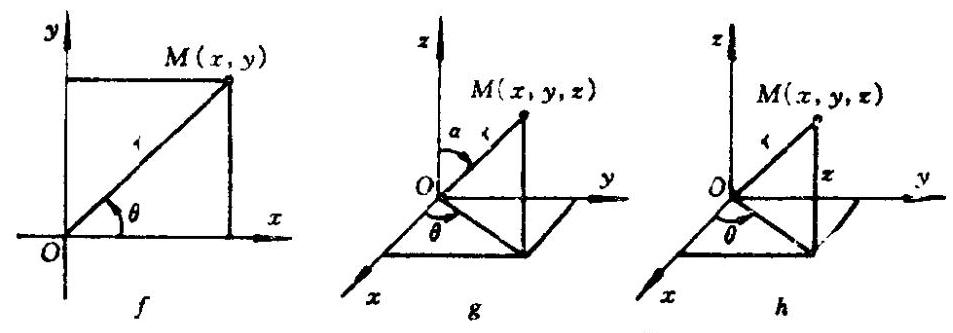
\includegraphics[max width=0.8\textwidth]{images/bo_d25ksc77aajc738obdgg_517_365_1263_953_333_0.jpg}
\end{center}
\hspace*{3em} 

图 10-10

关于 $k$ 元向量值函数的极限与连续性的运算性质,我们有下述定理。

定理 ${10} \cdot  3 \cdot  5$ 设 $f,g : A\left( { \subset  {\mathbf{R}}^{k}}\right)  \rightarrow  {\mathbf{R}}^{m}$ 是任意两个 $k$ 元向量值函数,并且当 $x \rightarrow  a$ 时极限 存在, $\lambda  : A\left( { \subset  {\mathbf{R}}^{k}}\right)  \rightarrow  \mathbf{R}$ 是 任一 $k$ 元实值函数,当 $x \rightarrow  a$ 时也有极限存在,则 $f + g : A \rightarrow  {\mathrm{R}}^{m},{\lambda f} :$  $A \rightarrow  {\mathbf{R}}^{m}$ 当 $x \rightarrow  a$ 时极限存在,并且
\begin{align*}
	&\mathop{\lim }\limits_{{x \rightarrow  a}}\left( {f + g}\right) \left( x\right)  = \mathop{\lim }\limits_{{x \rightarrow  a}}f\left( x\right)  + \mathop{\lim }\limits_{{x \rightarrow  a}}g\left( x\right) ,\\
	&\mathop{\lim }\limits_{{x \rightarrow  a}}\left( {\lambda f}\right) \left( x\right)  = \mathop{\lim }\limits_{{x \rightarrow  a}}\lambda \left( x\right)  \cdot  \mathop{\lim }\limits_{{x \rightarrow  a}}f\left( x\right) .
\end{align*}

此定理的证明我们也留给读者作为练习.

下面一个定理是关于一般度量空间中复合映射的连续性的.

定理 ${10} \cdot  3 \cdot  6$ 设 $\left( {X,d}\right) ,\left( {Y,D}\right)$ 与 $\left( {Z,\rho }\right)$ 是 任意三个 度量空间, $A \subset  X,B \subset  Y$ 是两个非空集合, $f : A \rightarrow  Y$ 与 $g : B \rightarrow  Z$ 是任意两个映射, 假设

1) $E = \operatorname{Dom}\left( {g \circ  f}\right)  \neq  \varnothing$ ,

2) ${x}_{0} \in  E,f$ 在 ${x}_{0}$ 处连续, $g$ 在 ${y}_{0} = f\left( {x}_{0}\right)  \in  B$ 处连续, 则复合映射 $g \circ  f : E \rightarrow  Z$ 在 ${x}_{0}$ 处连续.

证明 重复定理 $4 \cdot  6 \cdot  3$ 的证明过程,并对 个 别记号稍作修改即可.

推论 若映射 $f : A \rightarrow  Y$ 在 $A$ 上连续,映射 $g : B \rightarrow  Z$ 在 $B$ 上连续,并且 $E = \operatorname{Dom}\left( {g \circ  f}\right)  \neq  \varnothing$ ,则复合映射 $g \circ  f : E \rightarrow  Z$ 在 $E$ 上连续.

作为这一段的结束, 我们来证明连续映射的一个 等价定义, 即下面定理.

定理 ${10} \cdot  3 \cdot  7$ 设(X, d)与(Y, D)是任意两个度量空间, $A \subset  X$ 是任一非空集合,则映射 $f : A \rightarrow  Y$ 在 $A$ 上连续的充分必要条件是:

若 $U$ 是 $Y$ 的任一开集,则 ${f}^{-1}\left( U\right)$ 是 $A$ 的开集.

证明 必要性 设 $f$ 在 $A$ 上连续, $U$ 是 $Y$ 的任一开集.

若 ${f}^{-1}\left( U\right)  = \varnothing$ ,则 ${f}^{-1}\left( U\right)$ 是 $A$ 的开集.

若 ${f}^{-1}\left( U\right)  \neq  \varnothing$ ,任取 $a \in  {f}^{-1}\left( U\right)$ ,我们证明存在 ${\delta }_{a} > 0$ 使得 $A \cap  {B}_{d}\left( {a,{\delta }_{a}}\right)  \subset  {f}^{-1}\left( U\right) .$

事实上,由于 $U$ 是开集,并且 $f\left( a\right)  \in  U$ ,故存在 $\varepsilon  > 0$ 使得 ${B}_{D}\left( {f\left( a\right) ,\varepsilon }\right)  \subset  U$ ,又因为 $f$ 在 $a$ 处连续,所以存在 ${\delta }_{a} > 0$ 使得
$$\forall x \in  A,d\left( {a,x}\right)  < {\delta }_{a} \Rightarrow  D\left( {f\left( x\right) ,f\left( a\right) }\right)  < \varepsilon .$$

此即等价于 $f\left( {A \cap  {B}_{1}\left( {a,{\delta }_{a}}\right) }\right)  \subset  {B}_{D}\left( {f\left( a\right) ,\varepsilon }\right)$ 或
$$A \cap  {B}_{d}\left( {a,{\delta }_{a}}\right)  \subset  {f}^{-1}\left( {{B}_{D}\left( {f\left( a\right) ,\varepsilon }\right) }\right)  \subset  {f}^{-1}\left( U\right) .$$

因为 $A \cap  {B}_{d}\left( {a,{\delta }_{a}}\right)  = {B}_{{d}_{A}}\left( {a,{\delta }_{a}}\right)$ 是 $A$ 的以 $a$ 为心以 ${\delta }_{a}$ 为半径的开球,故由 $a$ 的任意性推知, ${f}^{-1}\left( U\right)$ 是 $A$ 的开集.

充分性 设对 $Y$ 的任一开集 $U,{f}^{-1}\left( U\right)$ 是 $A$ 的开集,任取 $a \in  A$ ,于是 $\forall \varepsilon  > 0,{B}_{D}\left( {f\left( a\right) ,\varepsilon }\right)$ 是 $Y$ 的开集,从而由假设知 ${f}^{-1}\left( {{B}_{D}\left( {f\left( a\right) ,\varepsilon }\right) }\right)$ 是 $A$ 的开集,由于 $a \in  {f}^{-1}\left( {{B}_{D}\left( {f\left( a\right) ,\varepsilon }\right) }\right)$ , 故存在 ${\delta }_{a} > 0$ 使得
$${B}_{{d}_{A}}\left( {a,{\delta }_{a}}\right)  = A \cap  {B}_{d}\left( {a,{\delta }_{a}}\right)  \subset  {f}^{-1}\left( {{B}_{D}\left( {f\left( a\right) ,\varepsilon }\right) }\right) ,$$

或
$$f\left( {A \cap  {B}_{d}\left( {a,{\delta }_{a}}\right)  \subset  {B}_{D}\left( {f\left( a\right) ,\varepsilon }\right) .}\right.$$

此即等价于
$$\forall x \in  A,d\left( {a,x}\right)  < {\delta }_{a} \Rightarrow  D\left( {f\left( x\right) ,f\left( a\right) }\right)  < \bar{\varepsilon }.$$

因此 $f$ 在 $a$ 处连续. 由 $a$ 的任意性知, $f$ 在 $A$ 上连续.

下面我们介绍映射的一致连续性。

\section*{3. 映射的一致连续性}

定义 设(X, d)与(Y, D)是任意两个度量空间, $A \subset  X$ 是任一非空集合, $f : A \rightarrow  Y$ 是任一映射,我们称 $f$ 在 $A$ 上一致连续, 如果它具有下述性质:
\begin{align*}
	&\left( {\forall \varepsilon  > 0}\right) \left( {\exists \delta  > 0}\right) \left( {\forall x,{x}^{\prime } \in  A,d\left( {x,{x}^{\prime }}\right)  < \delta }\right)\\
	&\Rightarrow  D\left( {f\left( x\right) ,f\left( {x}^{\prime }\right) }\right)  < \varepsilon \text{ . }
\end{align*}

由这个定义可知,若 $f$ 在 $A$ 上一致连续,则 $f$ 在 $A$ 上连续,但反之则不然.

例 10 设二元函数 $f : {\mathbf{R}}^{2} \rightarrow  \mathbf{R}$ 定义如下:
$$\forall \left( {x,y}\right)  \in  {\mathrm{R}}^{2},f\left( {x,y}\right)  = \sin x{\sin }^{y}.$$

证明: $f$ 在 ${\mathbf{R}}^{2}$ 上一致连续.

事实上, $\forall \left( {x,y}\right) ,\left( {{x}^{\prime },{y}^{\prime }}\right)  \in  {\mathbf{R}}^{2}$ ,我们有
\begin{align*}
	&\left| {f\left( {x,y}\right)  - f\left( {{x}^{\prime },{y}^{\prime }}\right) }\right|  = \left| {\sin x\sin y - \sin {x}^{\prime }\sin {y}^{\prime }}\right|\\
	&\leq  \left| {\sin x\left( {\sin y - \sin {y}^{\prime }}\right) }\right|\\
	&+ \left| {\sin {y}^{\prime }\left( {\sin x - \sin {x}^{\prime }}\right) }\right|\\
	&\leq  \left| {\sin y - \sin {y}^{\prime }}\right|  + \left| {\sin x - \sin {x}^{\prime }}\right|\\
	&\leq  \left| {x - {x}^{\prime }}\right|  + \left| {y - {y}^{\prime }}\right| \text{ . }
\end{align*}

若在 ${\mathbf{R}}^{2}$ 中取基本度量 ${d}_{2}$ ,则
\begin{align*}
	&\left( {\forall \varepsilon  > 0}\right) \left( {\exists \delta  = \varepsilon  > 0}\right) \left( {\forall \left( {x,y}\right) ,\left( {{x}^{\prime },{y}^{\prime }}\right)  \in  {\mathbf{R}}^{2},}\right.\\
	&\left| {x - {x}^{\prime }}\right|  + \left| {y - {y}^{\prime }}\right|  < \delta\\
	&\Rightarrow  \left| {f\left( {x,y}\right)  - f\left( {{x}^{\prime },{y}^{\prime }}\right) }\right|  < \left| {x - {x}^{\prime }}\right|  + \left| {y - {y}^{\prime }}\right|  < \bar{\varepsilon }\text{ . }
\end{align*}

故 $f$ 在 ${\mathbf{R}}^{2}$ 上一致连续.

例11 设 $\left( {X,\parallel  \cdot  \parallel }\right)$ 是任一赋范向量空间,则范数映射 $x \mapsto  \parallel x\parallel ,x \in  X$ 在 $X$ 上一致连续.

为此设 $x,{x}^{\prime } \in  X$ ,则我们有不等式
$$\left| {\parallel x\parallel  - \begin{Vmatrix}{x}^{\prime }\end{Vmatrix}}\right|  \leq  \begin{Vmatrix}{x - {x}^{\prime }}\end{Vmatrix}.$$

于是
\begin{align*}
	&\left( {\forall \varepsilon  > 0}\right) \left( {\exists \delta  = \varepsilon  > 0}\right) \left( {\forall x,{x}^{\prime } \in  X,\begin{Vmatrix}{x - {x}^{\prime }}\end{Vmatrix} < \delta }\right)\\
	&\Rightarrow  \left| {\parallel x\parallel  - \begin{Vmatrix}{x}^{\prime }\end{Vmatrix}}\right|  \leq  \begin{Vmatrix}{x - {x}^{\prime }}\end{Vmatrix} < \varepsilon .
\end{align*}

因此范数映射 $x \mapsto  \parallel x\parallel ,x \in  X$ 在 $X$ 上一致连续.

例 12 设映射 $T : {C}^{0}\left( {\left\lbrack  {a,b}\right\rbrack  ,\mathbf{R}}\right)  \rightarrow  {C}^{0}\left( {\left\lbrack  {a,b}\right\rbrack  ,\mathbf{R}}\right)$ 定义如下:
$$\forall f \in  {C}^{0}\left( {\left\lbrack  {a,b}\right\rbrack  ,\mathbf{R}}\right) ,\left( {Tf}\right) \left( x\right)  = {\int }_{a}^{x}f\left( t\right) {dt},\;\forall x \in  \left\lbrack  {a,b}\right\rbrack  .$$

证明: $T$ 在 ${C}^{0}\left( {\left\lbrack  {a,b}\right\rbrack  \mathbf{R}}\right)$ 上关于一致收敛范数一致连续.

事实上, $\forall f,g \in  {C}^{0}\left( {\left\lbrack  {a,b}\right\rbrack  ,\mathrm{R}}\right)$ ,我们有
\begin{align*}
	&\parallel {Tf} - {Tg}{\parallel }_{\infty } = \mathop{\sup }\limits_{{x \in  \left\lbrack  {a,b}\right\rbrack  }}\left| {\left( {Tf}\right) \left( x\right)  - \left( {Tg}\right) \left( x\right) }\right|\\
	&= \mathop{\sup }\limits_{{x \in  \left\lbrack  {a,b}\right\rbrack  }}\left| {{\int }_{a}^{x}f\left( t\right) {dt} - {\int }_{a}^{x}g\left( t\right) {dt}}\right|\\
	&\leq  \left( {b - a}\right) \parallel f - g\parallel \ldots
\end{align*}

于是
\begin{align*}
	&\left( {\forall \varepsilon  > 0}\right) \left( {\exists \delta  = \frac{\widehat{\varepsilon }}{b - a} > 0}\right) \left( {\forall f,g \in  {C}^{0}(\left\lbrack  {a,b}\right\rbrack  ,\mathbf{R}}\right) ,\\
	&\parallel f - g{\parallel }_{\infty } < \delta )\\
	&\Rightarrow  \parallel {Tf} - {Tg}{\parallel }_{\infty } \leq  \left( {b - a}\right) \parallel f - g{\parallel }_{\infty } < \bar{\varepsilon },
\end{align*}

因此映射 $T$ 在 ${C}^{0}\left( {\left\lbrack  {a,b}\right\rbrack  ,\mathbf{R}}\right)$ 上一致连续

\section*{4. 度量空间的同胚映射}

定义 设(X, d)与(Y, D)是任意两个度量空间, $f : X \rightarrow  Y$ 是任一映射,若 $f$ 具有下述性质:

1) $f$ 是一一映射:

2) $f$ 与 ${f}^{-1} : Y \rightarrow  X$ 都是连续映射.

则我们称 $f$ 是一个同胚映射 (也可简称同胚),并称 $X$ 与 $Y$ 同胚.

由定义可知,若 $f : X \rightarrow  Y$ 与 $g : Y \rightarrow  Z(\left( {Z,\rho }\right)$ 是一度量空间) 都是同胚,则 $g \circ  f : X \rightarrow  Z$ 也是同胚。

例 13 考虑映射 $f : \rbrack  - 1,1\lbrack  \rightarrow  \mathbf{R}$ :
$$\forall x \in  \rbrack  - 1,1\lbrack ,f\left( x\right)  = \operatorname{tg}\frac{\pi }{2}x.$$

则 $f$ 是一个同胚映射,从而 $\rbrack  - 1,1\lbrack$ 与 $\mathbf{R}$ 同胚.

事实上, $f$ 是连续一一映射,其逆 ${f}^{-1} : \mathbf{R} \rightarrow  \rbrack  - 1,1\lbrack$ 为
$$\forall y \in  \mathbf{R},{f}^{-1}\left( y\right)  = \frac{2}{\pi }\operatorname{arctg}y.$$

显然 ${f}^{-1}$ 连续. 故 $f$ 是一个同胚映射,从而 $\rbrack  - 1,1\lbrack$ 与 $\mathbf{R}$ 同胚.

例 14 考虑 ${\mathbf{R}}^{3}$ 的单位球面 ${S}^{2}$ :
$${S}^{2} = \left\{  {\left( {x,y,z}\right)  \in  {\mathbf{R}}^{3} \mid  {x}^{2} + {y}^{2} + {z}^{2} = 1}\right\}  .$$

设 $M\left( {x,y,z}\right) \left( {M}^{\prime }\right)$ 是此球面上异于北极点 $N\left( {0,0,1}\right)$ (南极点 $S\left( {0,0, - 1}\right) )$ 的任意一点,联结点 $N\left( S\right)$ 与 $M\left( {M}^{\prime }\right)$ 的直线交 ${xOy}$ 平面 $\pi$ 上唯一一点 $P\left( {t,s,0}\right) \left( {Q\left( {u,v,0}\right) }\right)$ (如下图所示). 由于 $\pi$ 平面上每一点的第 3 坐标为 0,故可以认为 $\left( {t,s,0}\right)  = \left( {t,s}\right)$ ,

从而可恒等 $\pi$ 与 ${\mathbf{R}}^{2}$ .

\begin{center}
	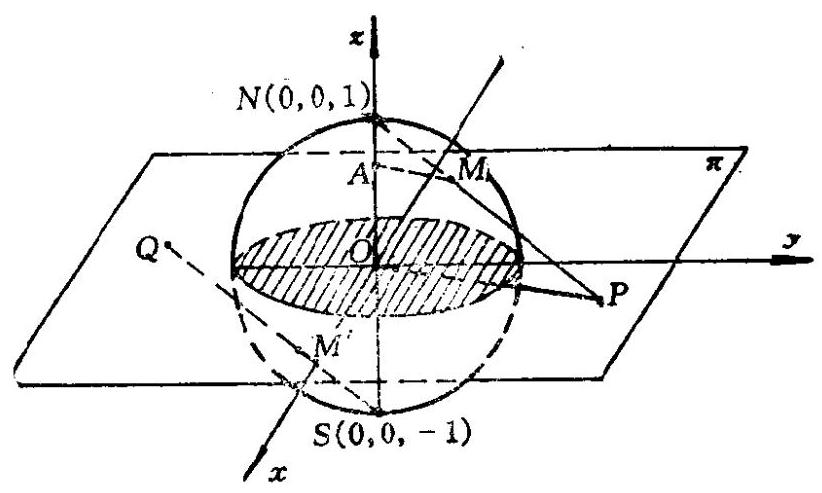
\includegraphics[max width=0.7\textwidth]{images/bo_d25ksc77aajc738obdgg_522_333_372_822_493_0.jpg}
\end{center}
\hspace*{3em} 

图 10-11

由此我们得到两个映射 $\Phi  : {S}^{2} - \{ N\}  \rightarrow  {\mathbf{R}}^{2}$ 与 $\Psi  : {S}^{2} - \{ S\}$

$\rightarrow  {\mathrm{R}}^{2}$ ,它们分别定义如下:
\begin{align*}
	&\forall M \in  {S}^{2} - \{ N\} ,\Phi \left( M\right)  = P,\\
	&\forall {M}^{\prime } \in  {S}^{2} - \{ S\} ,\Psi \left( {M}^{\prime }\right)  = Q.
\end{align*}

映射 $\Phi$ 与 $\Psi$ 分别称为单位球面 ${S}^{2}$ 关于北极点 $N$ 与南极点 $S$ 的球极投影.

下面我们来推导映射 $\Phi$ 的解析表达式.

由上图可得到下述明显比例关系式:
$$\frac{1 - z}{1} = \frac{\overline{AM}}{\overline{OP}} = \frac{x}{t} = \frac{y}{s}\;\left( {P \neq  0}\right) .$$

于是
$$\left\{  {\begin{array}{l} t = {\Phi }_{1}\left( {x,y,z}\right)  = \frac{x}{1 - z}, \\  s = {\Phi }_{2}\left( {x,y,z}\right)  = \frac{y}{1 - z}, \end{array}\;\forall \left( {x,y,z}\right)  \in  {S}^{2}-\{ N\} .}\right.$$

显然映射 $\Phi$ 在 ${S}^{2} - \{ N\}$ 上连续并且是一一映射.

我们记 $\Phi$ 的逆映射为 $\varphi  : {\mathbf{R}}^{2} \rightarrow  {S}^{2} - \{ N\}$ ,下面我们来推导 $\varphi$ 的解析表达式. 由
$${t}^{2} + {s}^{2} = \frac{{x}^{2} + {y}^{2}}{{\left( 1 - z\right) }^{2}} = \frac{1 - {z}^{2}}{{\left( 1 - z\right) }^{2}} = \frac{1 + z}{1 - z}$$

解得
$$z = \frac{{t}^{2} + {s}^{2} - 1}{1 + {t}^{2} + {s}^{2}}.$$

将它代入 $t,s$ 的表达式中得到
$$x = \frac{2t}{1 + {t}^{2} + {s}^{2}},y = \frac{2s}{1 + {t}^{2} + {s}^{2}}.$$

因此 $\varphi  : {\mathbf{R}}^{2} \rightarrow  {S}^{2} - \{ N\}$ 的解析表达式为
$$\varphi \left( {t,s}\right)  = \left( {\frac{2t}{1 + {t}^{2} + {s}^{2}},\frac{2s}{1 + {t}^{2} + {s}^{2}},\frac{{t}^{2} + {s}^{2} - 1}{1 + {t}^{2} + {s}^{2}}}\right) ,$$

$\forall \left( {t,s}\right)  \in  {\mathbf{R}}^{2}$ .

由此可知,映射 $\varphi$ 在 ${\mathbf{R}}^{2}$ 上也是连续的,故 $\Phi  : {S}^{2} - \{ \mathbf{N}\}  \rightarrow  \mathbf{R}$ 是一个同胚映射,从而 ${S}^{2} - \{ N\}$ 与 ${\mathbf{R}}^{2}$ 同胚.

同理可证,映射 $\Psi  : {S}^{2} - \{ S\}  \rightarrow  {\mathbf{R}}^{2}$ 也是同胚映射. 从而 ${S}^{2}$  $- \{ S\}$ 与 ${\mathbf{R}}^{2}$ 同胚,并且 $\Psi$ 与它的逆映射 $\psi  : {\mathbf{R}}^{2} \rightarrow  {S}^{2} - \{ S\}$ 的解析表达式为:
$$\left\{  {\begin{array}{l} u = {\Psi }_{1}\left( {x,y,z}\right)  = \frac{x}{1 + z}, \\  v = {\Psi }_{2}\left( {x,y,z}\right)  = \frac{y}{1 + z}, \end{array}\forall \left( {x,y,z}\right)  \in  {S}^{2}-\{ S\} ,}\right.$$

与
\begin{align*}
	&\psi \left( {u,v}\right)  = \left( {\frac{2u}{1 + {u}^{2} + {v}^{2}},\frac{2v}{1 + {u}^{2} + {v}^{2}},\frac{1 - {u}^{2} - {v}^{2}}{1 + {u}^{2} + {v}^{2}}}\right) ,\\
	&\forall \left( {u,v}\right)  \in  {\mathbf{R}}^{2}.
\end{align*}

例 15 设 ${S}^{1}$ 是平面上的单位圆周:
$${S}^{1} = \left\{  {\left( {x,y}\right)  \in  {\mathbf{R}}^{2} \mid  {x}^{2} + {y}^{2} = 1}\right\}  ,$$

映射 $f : \left\lbrack  {0,1\left\lbrack  { \rightarrow  {S}^{1}}\right. }\right.$ 定义为
$$\forall t \in  \lbrack 0,1\lbrack ,f\left( t\right)  = \left( {\cos {2\pi t},\sin {2\pi t}}\right) .$$

容易证明 $f$ 是连续的一一映射,但 $f$ 的逆映射 ${f}^{-1}$ 不是连续映射 (见习题第 14 题),因此 $f$ 不是同胚映射. 能否由此 断定 $\lbrack 0,1\lbrack$ 与 ${S}^{1}$ 不同胚? 为什么?

\section*{习 题}

1. 设(X, d)是任一度量空间, $\left\langle  {x}_{n}\right\rangle$ 是 $X$ 的任一点序列, $a \in  X$ 称为 $\left\langle  {x}_{n}\right\rangle$ 的极限点,如果

$\left( {\forall U \in  \mathcal{N}\left( a\right) }\right) \left( {\forall k \in  N}\right) \left( {\exists n \in  N,n \geq  k}\right)  \Rightarrow  {x}_{n} \in  U.$

1) 证明: $a$ 是 $\left\langle  {x}_{n}\right\rangle$ 的极限点当且仅当 $\left\langle  {x}_{n}\right\rangle$ 有收敛于 $a$ 的子序列 $\left\langle  {x}_{{k}_{n}}\right\rangle$ .

2) 证明: 若 $\mathop{\lim }\limits_{{n \rightarrow   + \infty }}{x}_{n} = a$ ,则 $a$ 是 $\left\langle  {x}_{n}\right\rangle$ 的唯一极限点.

2. 设 $M$ 是所有 $k \times  k$ 实矩阵的集合, $\forall A \in  M$ 令
$$A = \left( \begin{matrix} {a}_{11} & {a}_{12} & \cdots & {a}_{1k} \\  {a}_{21} & {a}_{22} & \cdots & {a}_{2k} \\  \cdots & \cdots & \cdots & \cdots \\  {a}_{k1} & {a}_{k2} & \cdots & {a}_{kk} \end{matrix}\right) ,\;\parallel A\parallel  = \mathop{\sum }\limits_{{i = 1}}^{k}\mathop{\sum }\limits_{{j = 1}}^{k}\left| {a}_{ij}\right| .$$

1) 证明: 如此定义的映射 $\parallel  \cdot  \parallel  : M \rightarrow  {R}^{ + }$ 是 $M$ 上的一个范数,因此 $\left( {M,\parallel  \cdot  \parallel }\right)$ 是一赋范空间.

2) 证明: 若 $\left\langle  {A}_{n}\right\rangle$ 收敛于 $A,\left\langle  {B}_{n}\right\rangle$ 收敛于 $B$ ,则 $\left\langle  {{A}_{n}{B}_{n}}\right\rangle$ 收敛于 ${AB}$ .

3) 设 $\left\langle  {A}_{n}\right\rangle$ 是 $M$ 的可逆矩阵序列,并且 $\left\langle  {A}_{n}\right\rangle$ 收敛于不可逆矩阵 $A$ . 证明: $\mathop{\lim }\limits_{{n \rightarrow   + \infty }}\begin{Vmatrix}{A}_{n}^{-1}\end{Vmatrix} =  + \infty$ .

3. 设(X, d)是任一度量空间, $A \subset  X$ 是任一非空集合, $a \in  X$ ,我们称实数
$$d\left( {a,A}\right)  = \mathop{\inf }\limits_{{x \in  A}}d\left( {a,x}\right)$$

\section*{为 $a$ 与 $A$ 的距离}

1) 证明: $a \in  \bar{A} \Leftrightarrow  d\left( {a,A}\right)  = 0$ .

2) 证明: 映射 $x \mapsto  d\left( {x,A}\right) ,x \in  X$ ,是 Lipschitz 系数为 1 的 Lipschitz 映射,即
$$\forall x,y \in  X,\left| {d\left( {x,A}\right)  - d\left( {y,A}\right) }\right|  \leq  d\left( {x,y}\right) .$$

4. 设(X, d)是任一度量空间, $A \subset  X$ 是任一非空集合. 我们称实数
$$d\left( A\right)  = \mathop{\sup }\limits_{x}d\left( {x,y}\right)$$

为集合 $A$ 的直径,在 ${X}^{2} \times  {X}^{2}$ 上定义映射 $\rho$ 如下:
$$\forall \left( {x,y}\right) ,\left( {{x}^{\prime },{y}^{\prime }}\right)  \in  {X}^{2},$$

$\cdots \left( {x,y}\right) ,\left( {{x}^{\prime },{y}^{\prime \prime }}\right)  = d\left( {x,{x}^{\prime }}\right)  + d\left( {y,{y}^{\prime }}\right) .$

1) 证明: $\left( {{X}^{2},\rho }\right)$ 是一个变量空间.

2) 证明: 映射 $\left( {x,y}\right)  \mapsto  d\left( {x,y}\right) ,\left( {x,y}\right)  \in  {X}^{2}$ ,在 ${X}^{2}$ 上连续.

3) 证明: $d\left( A\right)  = d\left( A\right)$ .

5. 设(X, d)是任一度量空间, $\mathcal{F}$ 是 $X$ 的所有有界闭集的集合,我们在 $\mathcal{F}$ 上定义Hausdorff度量 $A$ . 为此, $\forall A,B \in  \mathcal{F}$ ,令
$$\lambda \left( {A,B}\right)  = \mathop{\sup }\limits_{{x \in  A}}d\left( {x,B}\right) ,\Delta \left( {A,B}\right)  = \max \left( {\lambda \left( {A,B}\right) ,\lambda \left( {B,A}\right) }\right) .$$

证明: 1) $\lambda \left( {A,B}\right)  = 0 \Leftrightarrow  A \subset  B$ ;

2) $\forall A,B,C \in  \mathcal{F},\lambda \left( {A,C}\right)  \leq  \lambda \left( {A,B}\right)  + \lambda \left( {B,C}\right)$ ;

3) $\Delta$ 是 $\mathcal{F}$ 上的一个度量;

4) 映射 $\delta  : \mathcal{F} \rightarrow  \mathrm{R}\left( {\forall A \in  \mathcal{F},\delta \left( A\right)  = d\left( A\right) }\right)$ 连续.

6. 设(X, d)与(Y, D)是两个度量空间, $f : X \rightarrow  Y$ 是任一映射,则下述结论等价:

1) $f$ 在 $X$ 上连续;

2) 对(Y, D)中任一闭集 $F$ , ${f}^{-1}\left( F\right)$ 是(X, d)中的闭集;

3) 对任一集合 $A \subset  X,f\left( \bar{A}\right)  \subset  \overline{f\left( A\right) }$ .

7. 设 $A \subset  {R}^{2}$ 是任一开集, $f : A \rightarrow  R$ 满足下述条件:

1) $f$ 分别关于 $x$ 与 $y$ 连续,

2) $f$ 对其中一个变元是单调的.

证明 $f$ 在 $A$ 上连续.

8. 设函数 $f : {R}^{2} \rightarrow  R$ 定义如下:
$$f\left( {x,y}\right)  = \left\{  \begin{matrix} \frac{{\left| xy\right| }^{\lambda }}{{x}^{2} + {y}^{2}}, & \text{ 若 }\left( {x,y}\right)  \neq  \left( {0,0}\right) ,\left( {\lambda  \in  \mathrm{R}}\right) ; \\  0, & \text{ 若 }\left( {x,y}\right)  = \left( {0,0}\right) . \end{matrix}\right.$$

研究 $f$ 在(0,0)处的连续性.

9. 设函数 $f : {R}^{3} \rightarrow  R$ 定义如下:
$$f\left( {x,y,z}\right)  = \left\{  \begin{matrix} \frac{{x}^{3} + {y}^{3} + {z}^{3}}{\sqrt{{x}^{2} + {y}^{2} + {z}^{2}}}, & \text{ 若 }\left( {x,y,z}\right)  \neq  \left( {0,0,0}\right) \\  0 & \text{ 若 }\left( {x,y,z}\right)  = \left( {0,0,0}\right) . \end{matrix}\right.$$

研究 $f$ 在(0,0,0)处的连续性.

10. 设 $D \subset  {R}^{2}$ 是任一开集, $\left( {a,b}\right)  \in  D,f : D \rightarrow  R$ 是任一函数,我们称 $\mathop{\lim }\limits_{{\left( {x,y}\right)  \rightarrow  \left( {a;b}\right) }}f\left( {x,y}\right)$ 为全面极限,而 $\mathop{\lim }\limits_{{y \rightarrow  b}}f\left( {x,y}\right)$ ) 与 $\mathop{\lim }\limits_{{x \rightarrow  a}}f\left( {x,y}\right)$ ) 与 $\mathop{\lim }\limits_{{x \rightarrow  a}}$

$f\left( {x,y}\right) )$ 为累次极限. 证明: 若

1) $\mathop{\lim }\limits_{{\left( {x,y}\right)  \rightarrow  \left( {a;b}\right) }}f\left( {x,y}\right)  = A$ 存在,

2) $\forall y,\mathop{\lim }\limits_{{x \rightarrow  a}}f\left( {x,y}\right)  = h\left( y\right)$ 存在,

则累次极限 $\mathop{\lim }\limits_{{y \rightarrow  b}}\left( {\mathop{\lim }\limits_{{x \rightarrow  a}}f\left( {x,y}\right) }\right)$ 存在,并且
$$\mathop{\lim }\limits_{{\left( {x;y}\right)  \rightarrow  \left( {a;b}\right) }}f\left( {x,y}\right)  = \mathop{\lim }\limits_{{y \rightarrow  b}}\left( {\mathop{\lim }\limits_{{x \rightarrow  a}}f\left( {x,y}\right) }\right)  = A.$$

11. 设函数 $f : {R}^{2} \rightarrow  R$ 定义如下:
$$f\left( {x,y}\right)  = \left\{  \begin{matrix} \frac{{x}^{2}{y}^{2}}{{x}^{2}{y}^{2} + {\left( x - y\right) }^{2}}, & \left( {x,y}\right)  = \left( {0,0}\right) , \\  0, & \left( {x,y}\right)  = \left( {0,0}\right) . \end{matrix}\right.$$

证明: 累次极限 $\mathop{\lim }\limits_{{x \rightarrow  0}}\left( {\mathop{\lim }\limits_{{y \rightarrow  0}}f\left( {x,y}\right) }\right)  = \mathop{\lim }\limits_{{y \rightarrow  0}}\left( {\mathop{\lim }\limits_{{x \rightarrow  0}}f\left( {x,y}\right) }\right)  = 0$ ,但全面极限 $\mathop{\lim }\limits_{{\left( {x,y}\right)  \rightarrow  \left( {0;0}\right) }}f\left( {x,y}\right)$ 不存在.

12. 设函数 $f : {R}^{2} \rightarrow  R$ 定义如下:
$$f\left( {x,y}\right)  = \left\{  \begin{matrix} \left( {x + y}\right) \sin \frac{1}{x}\sin \frac{1}{y}, & x \neq  0,y \neq  0, \\  0, & x = 0\text{ 或 }y = 0. \end{matrix}\right.$$

证明: 累次极限 $\mathop{\lim }\limits_{{x \rightarrow  0}}\left( {\mathop{\lim }\limits_{{y \rightarrow  0}}f\left( {x,y}\right) }\right)$ 与 $\mathop{\lim }\limits_{{y \rightarrow  0}}\left( {\mathop{\lim }\limits_{{x \rightarrow  0}}f\left( {x,y}\right) }\right)$ 不存在,但全面极限 $\mathop{\lim }\limits_{{\left( {x,y}\right)  \rightarrow  \left( {0;0}\right) }}f\left( {x,y}\right)$ 存在.

13. 计算下列各极限:

1) $\mathop{\lim }\limits_{{x \rightarrow  0}}\frac{\sin {xy}}{x}$ , 2) $\mathop{\lim }\limits_{{\left( {x,y}\right)  \rightarrow  \left( {0,0}\right) }}{y}^{2}\log \left( {{x}^{2} + {y}^{2}}\right)$ ,

3) $\mathop{\lim }\limits_{{\left( {x : y}\right)  \rightarrow  0;0}}\frac{\log \left( {1 + {xy}}\right)  - {xy}}{{x}^{2}{y}^{2}}$ ,

4) $\mathop{\lim }\limits_{{x \rightarrow  0 \rightarrow  0 : 0}}\frac{x{\left( x + y\right) }^{p}}{{\left( {x}^{2} + {y}^{2}\right) }^{3/2}}\cos \frac{1}{\sqrt{{x}^{2} + {y}^{2}}}\left( {p \geq  2}\right)$ ,

5) $\mathop{\lim }\limits_{{\left( {x,y}\right)  \rightarrow  \left( {+\infty , + \infty }\right) }}{\left( \frac{xy}{{x}^{2} + {y}^{2}}\right) }^{{x}^{2}}$

6) $\mathop{\lim }\limits_{{\left( {x : y}\right)  \rightarrow  \left( {+\infty ;0}\right) }}{\left( 1 + \frac{1}{x}\right) }^{\frac{{x}^{2}}{x + y}}$

14. 证明: 例 15 的映射 $f$ 的逆映射 ${f}^{-1}$ 不是连续映射.

15. 证明: $\mathrm{R}$ 中所有非空开区间都是同胚的.

16. 设(X, d)与(Y, D)是两个度量空间, $f : X \rightarrow  Y$ 是任一映射. 我们称 $f$ 是开(闭)映射,如果 $A$ 是 $X$ 中的开(闭)集. 则 $f\left( A\right)$ 是 $Y$ 中的开(闭)集.

现设 $f : X \rightarrow  Y$ 是一一映射. 证明下述结论互相等价:

1) $f$ 是同胚映射;

2) $f$ 是连续的开映射;

3) $f$ 是连续的闭映射.

\section{完备度量空间}

在第 3 章 § 4 中我们定义了 Cauchy 实数序列, 利用它研究了实数集 $\mathbf{R}$ 的完备性. 对一般度量空间(X, d)也可以引进 Cauchy 序列的概念,并利用它来研究(X, d)的完备性.

\section*{1. Cauchy 序列}

定义 设(X, d)是任一度量空间, $\left\langle  {x}_{n}\right\rangle$ 是 $X$ 的任一点序列, 我们称 $\left\langle  {x}_{n}\right\rangle$ 是 Cauchy 序列,如果
$$\left( {\forall \varepsilon  > 0}\right) \left( {\exists N \in  \mathbf{N}}\right) \left( {\forall n,k \in  \mathbf{N},n \geq  N}\right)$$

$\Rightarrow  d\left( {{x}_{n + k},{x}_{n}}\right)  < \varepsilon$ .

显然,若点序列 $\left\langle  {x}_{n}\right\rangle$ 收敛,则 $\left\langle  {x}_{n}\right\rangle$ 是 Cauchy 序列. 反之则不然. 但如果我们考虑的度量空间是 $\left( {{\mathbf{R}}^{k},{d}_{i}}\right)$ ,则另当别沦,即成立下面的定理.

定理 ${10} \cdot  4 \cdot  1\left( {\mathrm{R}}^{k}\right.$ 中的Cauchy收敛准则 $\left( {{\mathrm{R}}^{k},{d}_{i}}\right)$ 中的点序列 $\left\langle  {x}_{n}\right\rangle$ 收敛的充分必要条件是: $\left\langle  {x}_{n}\right\rangle$ 为 Cauchy 序列.

证明 $k = 1$ 时,结论已经证明了. 以下设 $k > 1$ .

必要性 显然.

充分性 设 $\left\langle  {x}_{n}\right\rangle$ 是 $\left( {{\mathrm{R}}^{k},{d}_{i}}\right)$ 的任一Cauchy序列,不失一般性,我们可以取 ${d}_{2}$ . 于是
\begin{align*}
	&\left( {\forall \varepsilon  > 0}\right) \left( {\exists N \in  \mathbf{N}}\right) \left( {\forall n,m \in  \mathbf{N},n > N}\right)\\
	&\Rightarrow  {d}_{2}\left( {{x}_{n + m},{x}_{n}}\right)  < \varepsilon .\\
	&{x}_{n} = \left( {{x}_{n1},{x}_{n2},\cdots ,{x}_{nk}}\right) \left( {\forall n \in  \mathbf{N}}\right) .
\end{align*}

则由 ${d}_{2}\left( {{x}_{n + m},{x}_{n}}\right)  < \varepsilon$ 推知
$$\forall n,m \in  N,n \geq  N \Rightarrow  \left\{  \begin{array}{l} \left| {{x}_{n + {m1}} - {x}_{n1}}\right|  < \bar{\varepsilon }, \\  \left| {{x}_{n + {m2}} - {x}_{n2}}\right|  < \varepsilon , \\  \cdots \cdots \cdots \cdots \cdots \cdots \\  \left| {{x}_{n + {mk}} - {x}_{nk}}\right|  < \bar{\varepsilon }. \end{array}\right.$$

此即表明 $\forall i = 1,2,\cdots ,k$ ,实数序列 $\left\langle  {x}_{ni}\right\rangle$ 是 $\mathbf{R}$ 的 Cauchy 序列. 根据 $\mathbf{R}$ 的Cauchy收敛准则知,每一个序列 $\left\langle  {x}_{n1}\right\rangle$ 收敛. 令.
$$\mathop{\lim }\limits_{{n \rightarrow   + \infty }}{x}_{ni} = \xi ,\;\left( {i = 1,2,\cdots ,k}\right) .$$

根据定理 ${10} \cdot  3 \cdot  1,{\mathbf{R}}^{k}$ 中的点序列 $\left\langle  {x}_{n}\right\rangle$ 收敛于 $\xi  = \left( {{\xi }_{1},{\xi }_{2},\cdots }\right.$ , $\left. {\xi }_{k}\right)  \in  {\mathbf{R}}^{k}$ . ∎

推论 复数空间 $\left( {\mathbf{C},\left| \cdot \right| }\right)$ 的点序列 $\left\langle  {z}_{n}\right\rangle$ 收敛的充分 必要条件是 $\left\langle  {z}_{n}\right\rangle$ 为 Cauchy 序列.

证明 令 ${z}_{n} = {x}_{n} + i{y}_{n}$ ,则

$\left\langle  {z}_{n}\right\rangle$ 是 Cauchy 序列当且仅当 $\left\langle  {x}_{n}\right\rangle$ 与 $\left\langle  {y}_{n}\right\rangle$ 是 Cauchy 实数序列, 因此推论成立.

下面我们研究的是除了 $\left( {{\mathbf{R}}^{k},{d}_{i}}\right)$ 与 $\left( {\mathbf{C},\left| \cdot \right| }\right)$ 外还有哪些一般度量空间具有 “Cauchy 序列均收敛” 这一好性质的. 为此引入下述概念.

\section*{2. 完备度量空间}

定义 设(X, d)是任一度量空间. 我们称它是完备的,如果它的任一Cauchy序列都是收敛的.

根据这一定义及定理 ${10} \cdot  4 \cdot  1$ 知, $\forall k \in  \mathbf{N},\left( {{\mathbf{R}}^{k},{d}_{i}}\right) ,\left( {\mathbf{C},\left| \cdot \right| }\right)$ 都是完备的度量空间.

下面是另一个典型的完备度量空间的例子.

例 1 在 ${C}^{0}\left( {\left\lbrack  {a,b}\right\rbrack  ,\mathrm{C}}\right)$ 上取一致度量 $d$ :

$\forall f,g \in  {C}^{0}\left( {\left\lbrack  {a,b}\right\rbrack  ,\mathrm{C}}\right) ,d\left( {f,g}\right)  = \mathop{\sup }\limits_{{x \in  \left\lbrack  {a,b}\right\rbrack  }}\left| {f\left( x\right)  - g\left( x\right) }\right| ,$ 则 $\left( {{C}^{c}\left( {\left\lbrack  {a,b}\right\rbrack  ,\mathrm{C}}\right) ,d}\right)$ 是完备度量空间.

为此设 $\left\langle  {f}_{n}\right\rangle$ 是 $\left( {{C}^{0}\left( {\left\lbrack  {a,b}\right\rbrack  ,C}\right) ,d}\right)$ 的任一 Cauchy 序列.

于是
\begin{align*}
	&\left( {\forall \varepsilon  > 0}\right) \left( {\exists N \in  \mathbf{N}}\right) \left( {\forall n,k \in  \mathbf{N},n \geq  N}\right)\\
	&\Rightarrow  d\left( {{f}_{n + k},{f}_{n}}\right)  = \mathop{\sup }\limits_{{x \in  \left\lbrack  {a,b}\right\rbrack  }}\left| {{f}_{n + k}\left( x\right)  - {f}_{n}\left( x\right) }\right|  < \varepsilon .
\end{align*}

由此推得
\begin{align*}
	&\left( {\forall n,k \in  \mathbf{N},n \geq  N}\right) \left( {\forall x \in  \left\lbrack  {a,b}\right\rbrack  }\right)\\
	&\Rightarrow  \left| {{f}_{n + k}\left( x\right)  - {f}_{n}\left( x\right) }\right|  < \varepsilon .
\end{align*}
(*)

此即表明 $\forall x \in  \left\lbrack  {a,b}\right\rbrack$ ,复数序列 $\left\{  {{f}_{n}\left( x\right) }\right\}$ 是 $\mathrm{C}$ 中的Cauchy 序列,由 $\left( {\mathrm{C},\left| \cdot \right| }\right)$ 的完备性知 $\left\langle  {{f}_{n}\left( x\right) }\right\rangle$ 收敛,于是我们可定义函数 $f : \left\lbrack  {a,b}\right\rbrack   \rightarrow  \mathbf{R}$ 如下:
$$\forall x \in  \left\lbrack  {a,b}\right\rbrack  ,f\left( x\right)  = \mathop{\lim }\limits_{{n \rightarrow   + \infty }}{f}_{n}\left( x\right) .$$

现在在 $\left( *\right)$ 式中固定 $n \rightarrow  N$ ,令 $k \rightarrow   + \infty$ 得到
\begin{align*}
	&\left( {\forall n \in  N,n \geq  N}\right) \left( {\forall x \in  \left\lbrack  {a,b}\right\rbrack  }\right)\\
	&\Rightarrow  \left| {f\left( x\right)  - {f}_{n}\left( x\right) }\right|  \leq  \varepsilon .\\
	&\left( {* * }\right)
\end{align*}

下面首先证明 $f \in  {C}^{0}\left( {\left\lbrack  {a,b}\right\rbrack  ,\mathrm{C}}\right)$ .

任取 ${x}_{0} \in  \left\lbrack  {a,b}\right\rbrack$ . 由于上述 $\left( {* * }\right) ,\forall x \in  \left\lbrack  {a,b}\right\rbrack$ 我们有:
\begin{align*}
	&\left| {f\left( x\right)  - f\left( {x}_{0}\right) }\right|\\
	&\leq  \left| {f\left( x\right)  - {f}_{N}\left( x\right) }\right|  + \left| {{f}_{N}\left( x\right)  - {f}_{N}\left( {x}_{0}\right) }\right|  + \left| {{f}_{N}\left( {x}_{0}\right)  - f\left( {x}_{0}\right) }\right|\\
	&< \varepsilon  + \left| {{f}_{N}\left( x\right)  - {f}_{N}\left( {x}_{0}\right) }\right|  + \varepsilon\\
	&= {2\varepsilon } + \left| {{f}_{N}\left( x\right)  - {f}_{N}\left( {x}_{0}\right) }\right| .
\end{align*}

因为 ${f}_{N} \in  {C}^{0}\left( {\left\lbrack  {a,b}\right\rbrack  ,\mathrm{C}}\right)$ ,故
\begin{align*}
	&\left( {\forall \varepsilon  > 0}\right) \left( {\exists \delta  > 0}\right) \left( {\forall x \in  \left\lbrack  {a,b}\right\rbrack   \cap  B\left( {{x}_{0},\delta }\right) }\right)\\
	&\Rightarrow  \left| {{f}_{N}\left( x\right)  - {f}_{N}\left( {x}_{0}\right) }\right|  < \varepsilon\\
	&\Rightarrow  \left| {f\left( x\right)  - f\left( {x}_{0}\right) }\right|  < {3\varepsilon }.
\end{align*}

因此 $f$ 在 ${x}_{0}$ 处连续. 由 ${x}_{0}$ 的任意性知 $f \in  {C}^{0}\left( {\left\lbrack  {a,b}\right\rbrack  ,\mathbf{C}}\right)$ .

最后证明 $d\left( {{f}_{n},f}\right)  \rightarrow  0\left( {n \rightarrow   + \infty }\right)$ .

事实上,由于
$$d\left( {{f}_{n},f}\right)  = \mathop{\sup }\limits_{{x \in  \left\lbrack  a\right\rbrack  }}\left| {{f}_{n}\left( x\right)  - f\left( x\right) }\right| ,$$

故由 $\left( {* * }\right)$ 式知, $\forall n \in  \mathbf{N},n \geq  N,d\left( {{f}_{n},f}\right)  \leq  \varepsilon$ . 此即表明 $d\left( {{f}_{n},f}\right)  \rightarrow  0\left( {n \rightarrow   + \infty }\right) .$

综合上述所证, Cauchy序列 $\left\langle  {f}_{n}\right\rangle$ 收敛于 $f$ . 因此 $\left( {{C}^{0}(\left\lbrack  {a,b}\right\rbrack  }\right.$ , C), $d)$ 是完备的度量空间.

附注 我们说度量空间(X, d)是完备的,是相对于度量 $d$ 而言,因此可能出现这种情形: 同一基本集合 $X$ ,对度量 $d,\left( {X,d}\right)$ 是完备的,而对另一度量 $D,\left( {X,D}\right)$ 又不是完备的. 例如在同 $- {C}^{0}\left( {\left\lbrack  {a,b}\right\rbrack  ,\mathrm{C}}\right)$ 上,我们定义度量 $D$ 为:
\begin{align*}
	&\forall f,g \in  {C}^{0}\left( {\left\lbrack  {a,b}\right\rbrack  ,\mathrm{C}}\right) ,\\
	&D\left( {f,g}\right)  = {\int }_{a}^{b}\left| {f\left( x\right)  - g\left( x\right) }\right| {dx},
\end{align*}

可以证明 $\left( {{C}^{0}\left( {\left\lbrack  {a,b}\right\rbrack  ,\mathrm{C}}\right) ,D}\right)$ 不是完备的 (见习题第 4 题).

但如果 $d$ 与 $D$ 是等价度量,则

(X, d)是完备的 $\Leftrightarrow  \left( {X,D}\right)$ 是完备的.

非完备度量空间的最简单例子就是熟知的实数空间 $\left( {\mathbf{R},\left| \cdot \right| }\right)$ 的有理数子空间 $\left( {\mathbf{Q},{\left| \cdot \right| }_{\mathbf{Q}}}\right)$ .

\section*{3. 完备度量空间的不动点定理}

定理 ${10} \cdot  4 \cdot  2$ (Banach 不动点定理) 设(X, d)是一完备度量空间, $f : X \rightarrow  X$ 是一压缩映射,即

$\forall x,y \in  X,d\left( {f\left( x\right) ,f\left( y\right) }\right)  \leq  {\lambda d}\left( {x,y}\right) \left( {0 \leq  \lambda  < 1}\right)$ ,则存在唯一的 $a \in  X$ ,使得 $f\left( a\right)  = a$ .

证明 任取 ${x}_{0} \in  X$ ,令
$${x}_{1} = f\left( {x}_{0}\right) ,{x}_{2} = f\left( {x}_{1}\right) ,\cdots ,{x}_{n + 1} = f\left( {x}_{n}\right) \cdots$$

于是我们得到 $X$ 的点序列 $\left\langle  {x}_{n}\right\rangle$ .

下面证明 $\left\langle  {x}_{n}\right\rangle$ 是(X, d)的Cauchy序列.

首先,由 $f$ 的压缩性,我们有: $\forall n \in  \mathbf{N}$ ,
\begin{align*}
	&d\left( {{x}_{n},{x}_{n + 1}}\right)  = d\left( {f\left( {x}_{n - 1}\right) ,f\left( {x}_{n}\right) }\right)  \leq  {\lambda d}\left( {{x}_{n - 1},{x}_{n}}\right)\\
	&:  \leq  \cdots  \leq  {\lambda }^{n}d\left( {{x}_{0},{x}_{1}}\right) .
\end{align*}

因此 $\forall k \in  \mathbf{N}$ ,
\begin{align*}
	&d\left( {{x}_{n},{x}_{n + k}}\right)  \leq  \widetilde{d}\left( {{x}_{n},{x}_{n + 1}}\right)  + d\left( {{x}_{n + 1},{x}_{n + 2}}\right)  + \cdots\\
	&+ d\left( {{x}_{n + k - 1},{x}_{n + k}}\right)\\
	&\leq  \left( {{\lambda }^{n} + {\lambda }^{n + 1} + \cdots  + {\lambda }^{n + k - 1}}\right) d\left( {{x}_{0},{x}_{1}}\right)\\
	&< \frac{{\lambda }^{n}}{1 - \lambda }d\left( {{x}_{0},{x}_{1}}\right) .
\end{align*}

若 $d\left( {{x}_{0},{x}_{1}}\right)  = 0$ ,则 ${x}_{0} = f\left( {x}_{0}\right)$ .

若 $d\left( {{x}_{0},{x}_{1}}\right)  \neq  0$ ,则 $\forall \varepsilon  > 0$ ,由 $\frac{{\lambda }^{n}}{1 - \lambda }d\left( {{x}_{0},{x}_{1}}\right)  < \varepsilon$ 得到 $n >$

$\log \left( \frac{\varepsilon \left( {1 - \lambda }\right) }{d\left( {{x}_{0},{x}_{1}}\right) }\right) /\log \lambda$ . 令
$$N = 1 + \left\lbrack  {\log \left( \frac{\varepsilon \left( {1 - \lambda }\right) }{d\left( {{x}_{0},{x}_{1}}\right) }\right) /\log \lambda }\right\rbrack  ,$$

则 $\forall n,k \in  \mathbf{N},n \geq  N \Rightarrow  d\left( {{x}_{n},{x}_{n + k}}\right)  < \frac{{\lambda }^{n}}{1 - \lambda }d\left( {{x}_{0},{x}_{1}}\right)  < \bar{\varepsilon }$ .

此即表明 $\left\langle  {x}_{n}\right\rangle$ 是(X, d)的Cauchy序列.

因为(X, d)是完备的,所以 $\left\langle  {x}_{n}\right\rangle$ 在 $X$ 中收敛,令 $\mathop{\lim }\limits_{{n \rightarrow   + \infty }}{x}_{n} = a$ , 则 $a \in  X$ .

再证 $a$ 是 $f$ 的不动点,即 $a = f\left( a\right)$ .

由 $f$ 的压缩性知, $f$ 在 $X$ 上连续 (实际上还是一致连续的). 在 ${x}_{n + 1} = f\left( {x}_{n}\right)$ 的两边令 $n \rightarrow   + \infty$ 取极限得到 $a = f\left( a\right)$ .

最后证明不动点的唯一性.

假设存在 $b \in  X$ 使得 $b = f\left( b\right)$ 且 $b \neq  a$ ,那末
$$d\left( {a,b}\right)  = d\left( {f\left( a\right) ,f\left( b\right) }\right)  \leq  {\lambda d}\left( {a,b}\right) ,$$

由于 $0 \leq  \lambda  < 1$ ,故必有 $d\left( {a,b}\right)  = 0$ 或 $a = b$ ,矛盾. 因此 $a$ 是 $f$ 的唯一不动点.

附注 从定理的证明过程可知,若 $Y$ 是完备度量空间 $\left( {\lambda ,d}\right)$ 的闭集, $f : Y \rightarrow  Y$ 是一压缩映射,则存在 $f$ 的唯一不动点 $a \in  Y$ .

Banach 不动点定理是一个非常重要的定理, 它在微分方程、代数方程的求解, 计算数学的数值计算等许多数学研究领域中有着广泛的应用.

\section*{习 题}

1. 设(X, d)是任一度量空间, $\left\langle  {x}_{n}\right\rangle  ,\left\langle  {y}_{n}\right\rangle$ 是 $X$ 的两个点序列. 证明:

1) 若 $\left\langle  {x}_{n}\right\rangle  ,\left\langle  {y}_{n}\right\rangle$ 为 Cauchy 序列,则 $\left\langle  {d\left( {{x}_{n},{y}_{n}}\right) }\right\rangle$ 收敛.

2) 若 $\left\langle  {x}_{n}\right\rangle$ 是 Cauchy 序列, $d\left( {{x}_{n},{y}_{n}}\right)  \rightarrow  0\left( {n \rightarrow   + \infty }\right)$ ,则 $\left\langle  {y}_{n}\right\rangle$ 也是 Cauchy序列.

2. 设(X, d)是任一度量空间, $Y \subset  X$ 是任一非空集合. 证明:(X, d) 的子空间 $\left( {Y,{d}_{Y}}\right)$ 是完备的充分必要条件是 $Y$ 为 $X$ 的闭集.

3. 设(X, d)是任一度量空间, $A \subset  X$ 且 $A = \varnothing$ ,
$$d\left( A\right)  = \mathop{\sup }\limits_{{x;y \in  A}}d\left( {x,y}\right)$$

为集合 $A$ 的直径. 证明:(X, d)是完备的充分必要条件是: 对 $X$ 的任一列闭集 $\left\langle  {A}_{n}\right\rangle$ ,若
$${A}_{n + 1} \subset  {A}_{n},\mathop{\lim }\limits_{{n \rightarrow   + \infty }}d\left( {A}_{n}\right)  = 0,$$

则 $\mathop{\bigcap }\limits_{{n = 1}}^{{+\infty }}{A}_{n}$ 是单点集.

4. 在 ${C}^{0}\left( {\left\lbrack  {0,1}\right\rbrack  ,C}\right)$ 上定义度量 $D$ 如下:

$\forall f,g \in  {C}^{0}\left( {\left\lbrack  {0,1}\right\rbrack  ,C}\right) ,D\left( {f,g}\right)  = {\int }_{0}^{1}\left| {f\left( x\right)  - g\left( x\right) }\right| {dx}.$

1) $\forall n \in  \mathrm{N}$ ,定义函数 ${f}_{n} : \left\lbrack  {0,1}\right\rbrack   \rightarrow  \mathrm{C}$ 为
$${f}_{n}\left( x\right)  = \left\{  \begin{array}{ll} 1, & 0 \leq  x \leq  \frac{1}{2}; \\  0, & \frac{1}{2} + \frac{1}{n} \leq  x \leq  1; \\  1 - n\left( {x - \frac{1}{2}}\right) , & \frac{1}{2} \leq  x \leq  \frac{1}{2} + \frac{1}{n}. \end{array}\right.$$

证明: ${f}_{n} \in  {C}^{0}\left( {\left\lbrack  {0,1}\right\rbrack  ,C}\right)$ ,且 $D$ 是 ${C}^{0}\left( {\left\lbrack  {0,1}\right\rbrack  ,C}\right)$ 的度量.

2) 证明: $\left\langle  {f}_{n}\right\rangle$ 是 $\left( {{C}^{0}\left( {\left\lbrack  {0,1}\right\rbrack  ,C}\right) ,D}\right)$ 的一Cauchy序列,但 $\left\langle  {f}_{n}\right\rangle$ 在 $\left( {{C}^{0}\left( {\left\lbrack  {0,1}\right\rbrack  ,C}\right) ,D}\right)$ 中不收敛. 因此 $\left( {{C}^{0}\left( {\left\lbrack  {0,1}\right\rbrack  ,C}\right) ,D}\right)$ 不是完备度量空间.

5. 设(X, d)与(Y, D)是两个度量空间,其中(Y, D)是完备的, $A \subset  X$ 是 $X$ 的一稠密集 $\left( {\bar{A} = X}\right)$ .

证明: 若 $f : A \rightarrow  Y$ 是任一连续映射,则存在唯一的映射 $\widetilde{f} : X \rightarrow  Y$ 使得

1) $\widetilde{f}$ 在 $X$ 上一致连续, $2{\left. \widetilde{f}\right| }_{A} = {f}_{ * }$ 此 结 论称 为连续延拓定理, $\widetilde{f}$ 称为 $f$ 的延拓.

6. 设 $\left( {X,d}\right) ,\left( {Y,D}\right)$ 是两个度量空间, $f : X \rightarrow  Y$ 是一致连续映射.

1) 证明: 若 $\left\langle  {x}_{n}\right\rangle$ 是(X, d)的Cauchy序列,则 $\left\langle  {f\left( {x}_{n}\right) }\right\rangle$ 是(Y, D)的 Cauchy序列.

2) 证明:若 $f$ 是一一映射, ${f}^{-1}$ 是一致连续的,则(X, d)是完备的当且仅当(Y, D)是完备的.

7. 设(X, d)是完备度量空间, $f : X \rightarrow  X$ 是一映射,
$${f}^{0} = i{d}_{X},{f}^{n + 1} = f \circ  {f}^{n}\;\left( {\forall n \in  N}\right) .$$

证明: 若存在 $m \in  \mathbf{N}$ 使得 ${f}^{m} : X \rightarrow  X$ 是压缩映射,则 $f$ 存在唯一的不动点 $a \in  X$ 使得
$$\forall {x}_{0} \in  X,a = \mathop{\lim }\limits_{{n \rightarrow   + \infty }}{f}^{n}\left( {x}_{0}\right) .$$

8. 设 $\left( {X,d}\right) \text{ 、 }\left( {Y,D}\right)$ 是两个度量空间,(X, d)是完备的,映射 $f : X$  $\times  Y \rightarrow  X$ 满足下述两个条件:

1) 存在 $0 \leq  \lambda  < 1$ 使得 $\forall t \in  Y$ ,映射 ${f}_{t} : x \mapsto  f\left( {x,t}\right) ,x \in  X$ 是压缩系数为 $\lambda$ 的压缩映射,即
$$\forall x,y \in  X,d\left( {{f}_{l}\left( x\right) ,{f}_{l}\left( y\right) }\right)  \leq  {\lambda d}\left( {x,y}\right) ;$$

2) $\forall x \in  X$ ,映射 $t \mapsto  f\left( {x,t}\right) ,t \in  Y$ 是连续的. 证明(如果 ${a}_{t}$ 是 ${f}_{t}$ 的唯一不动点,则映射 $t \mapsto  {a}_{t},t \in  Y$ 在 $Y$ 上连续.

\section{紧度量空间}

从第 3 章 $§4$ 的Cantor有限覆盖定理 (定理 $3 \cdot  4 \cdot  7$ ) 知道, $\mathbf{R}$ 的有限闭区间的一个重要性质就是它具有有限开覆盖性. 现在我们 E一般度量空间中研究这种有限开覆盖性, 这就是下面介绍的紧基概念。

\section*{1. 紧度量空间与紧集概念}

定义 设(X, d)是任一度量空间, $A \subset  X$ 是任一非空集合, ${\left\{  {U}_{\lambda }\right\}  }_{\lambda  \in  \Lambda }$ 是 $X$ 的一族开集.

1) 若 $A \subset  \mathop{\bigcup }\limits_{{\lambda  \in  \Lambda }}{U}_{\lambda }$ ,则我们称 ${\left\{  {U}_{\lambda }\right\}  }_{\lambda  \in  \Lambda }$ 是 $A$ 的一个开覆盖.

2) 设 ${\left\{  {U}_{\lambda }\right\}  }_{\lambda  \in  \Lambda }$ 是 $A$ 的开覆盖,若存在有限个 ${U}_{{\lambda }_{1}},{U}_{{\lambda }_{2}},\cdots$ , ${U}_{\lambda m}$ 使得 $A \subset  \mathop{\bigcup }\limits_{{i = 1}}^{m}{U}_{\lambda i}$ ,则我们称 ${\left\{  {U}_{\lambda }\right\}  }_{\lambda  \in  \Lambda }$ 有有限的开子覆盖 $\left\{  {{U}_{{\lambda }_{1}},{U}_{{\lambda }_{2}},\cdots ,{U}_{{\lambda }_{m}}}\right\}  .$

定义 设(X, d)是任一度量空间.

1) 我们称(X, d)是紧度量空间,如果 $X$ 的任一开覆盖都有一个有限的开子覆盖.

2) 设 $Y \subset  X$ 是任一非空集合,我们称 $Y$ 是紧集,如果子空间 $\left( {Y,{d}_{Y}}\right)$ 是紧的.

\section*{2. 紧度量空间的性质}

首先我们给出紧度量空间与完备度量空间关系的下述性质.

定理 ${10} \cdot  5 \cdot  1$ 若(X, d)是紧度量空间,则(X, d)是完备的.

证明 用反证法证明. 假设(X, d)不是完备的. 于是存在 (X, d)的一个Cauchy序列 $\left\langle  {x}_{n}\right\rangle$ 使得它在 $X$ 中不收敛.

因此 $\forall y \in  X,\left\langle  {x}_{n}\right\rangle$ 不收敛于 $y$ . 从而存在 ${\varepsilon }_{y} > 0$ 使得
$$\left( {\forall n \in  \mathbf{N}}\right) \left( {\exists {k}_{n} \in  \mathbf{N},{k}_{n} \geq  n}\right)  \Rightarrow  d\left( {{x}_{{k}_{n}},y}\right)  > 2{\varepsilon }_{y}.$$

由于 $\left\langle  {x}_{n}\right\rangle$ 是 Cauchy 序列,故
\begin{align*}
	&\left( {\exists N \in  \mathbf{N}}\right) \left( {\forall n,m \in  \mathbf{N},n,m \geq  N}\right)\\
	&\Rightarrow  d\left( {{x}_{n},{x}_{m}}\right)  < {\bar{\varepsilon }}_{y}.
\end{align*}

取 $m = {k}_{N}$ ,则 $\forall n \in  \mathbf{N},n \geq  N$ 有
\begin{align*}
	&d\left( {{x}_{n},y}\right)  \geq  d\left( {{x}_{{k}_{N}},y}\right)  - d\left( {{x}_{n},{x}_{{k}_{N}}}\right)\\
	&> 2{\varepsilon }_{y} - {\varepsilon }_{y} = {\varepsilon }_{y}.
\end{align*}

由此可知,在开球 $B\left( {y,{\varepsilon }_{y}}\right)$ 中最多只包含 $\left\langle  {x}_{n}\right\rangle$ 的有限多项.

现在由 $y$ 的任意性, $X = \mathop{\bigcup }\limits_{{y \in  X}}B\left( {y,{\bar{\varepsilon }}_{y}}\right)$ . 因为(X, d)是紧的, 所以存在有限多个 ${y}_{1},{y}_{2},\cdots ,{y}_{m} \in  X$ 使得 $X = \mathop{\bigcup }\limits_{{i = 1}}^{m}B\left( {{y}_{i},{\varepsilon }_{{y}_{i}}}\right)$ . 由于每一个 $B\left( {{y}_{i},{\varepsilon }_{{y}_{i}}}\right)$ 最多只包含 $\left\langle  {x}_{n}\right\rangle$ 的有限多项,故 $\left\langle  {x}_{n}\right\rangle$ 就不是一个无穷点序列. 此矛盾说明(X, d)必是完备的.

这个定理的逆显然是不成立. 例如实数空间 $\left( {\mathrm{R},\left| \cdot \right| }\right)$ 是完备的, 但它不是紧的. 然而对定理再附加某些条件, 仍可以保证其紧性成立 (见习题第 2 题).

下面定理所述的性质可以作为紧度量空间的一个等价定义.

定理 ${10} \cdot  5 \cdot  2$ 度量空间(X, d)是紧的充分必要条件是 $X$ 的每一个点序列 $\left\langle  {x}_{n}\right\rangle$ 都有收敛的子序列.

证明 必要性. 设(X, d)是紧的. $\left\langle  {x}_{n}\right\rangle$ 是 $X$ 的任一点序列. 为了证明 $\left\langle  {x}_{n}\right\rangle$ 有收敛子序列,我们来证明下述结论成立.

$\left( {\exists \bar{x} \in  X}\right) \left( {\forall 1 > 0}\right) \left( {\exists {x}_{n\left( r\right) } \in  X}\right)  \Rightarrow  {x}_{n\left( r\right) } \in  B\left( {\bar{x},r}\right) .$

用反证法. 假设此结论不成立, 那末

$\left( {\forall y \in  X}\right) \left( {\exists {r}_{y} > 0}\right)$ 使得 $\forall n \in  \mathbf{N},{x}_{n} \in  B\left( {y,{r}_{y}}\right)$ . 于是 $X = \mathop{\bigcup }\limits_{{y \in  X}}B\left( {y,{r}_{y}}\right)$ . 由(X, d)的紧性知,存在有限多个 ${y}_{1}$ , ${y}_{2},\cdots ,{y}_{m} \in  X$ 使得 $X = \mathop{\bigcup }\limits_{{i = 1}}^{m}B\left( {{y}_{i},{r}_{{y}_{i}}}\right)$ .

然而这不可能,因为每一个 $B\left( {{y}_{i},{r}_{{y}_{i}}}\right)$ 中不包含任一 ${x}_{n}$ . 此矛盾说明上述结论成立.

取 $r = \frac{1}{k}\left( {k \in  \mathbf{N}}\right)$ ,于是存在 ${x}_{{n}_{k}}$ 使得 ${x}_{{n}_{k}} \in  B\left( {\bar{x},\frac{1}{k}}\right)$ . 我们可以假设 ${n}_{k} < {n}_{k + 1}$ ,于是我们得到 $\left\langle  {x}_{n}\right\rangle$ 的一个子序列 $\left\langle  {x}_{{n}_{k}}\right\rangle$ ,它显然收敛于 $\bar{x}$ .

为了证明充分性, 我们先来证 明一个可作 为独 立结 论的命题.

命题 若度量空间(X, d)的每一个点序列都有收敛的子序列,则对 $X$ 的任一开覆盖 ${\left\{  {U}_{\lambda }\right\}  }_{\lambda  \in  \Lambda }$ ,存在正数 $\beta$ (称为Lebesgue 数), 它具有下述性质:
$$\left( {\forall x \in  X}\right) \left( {\exists \lambda  \in  \Lambda }\right)  \Rightarrow  B\left( {x,\beta }\right)  \subset  {U}_{\lambda }.$$

证明 用反证法证明. 假设对 $X$ 的某一个开覆盖 ${\left\{  {U}_{\lambda }\right\}  }_{\lambda  \in  \Lambda }$ , 不存在具有上述性质的正数 $\beta$ . 那末
$$\left( {\forall n \in  \mathbf{N}}\right) \left( {\exists {x}_{n} \in  X}\right) \left( {\forall \lambda  \in  \Lambda }\right)  \Rightarrow  B\left( {{x}_{n},\frac{1}{n}}\right)  \subset  {U}_{\lambda }.$$

由此得到 $X$ 的一点序列 $\left\langle  {x}_{n}\right\rangle$ . 根据已知条件, $\left\langle  {x}_{n}\right\rangle$ 有收敛子序列 $\left\langle  {x}_{{n}_{k}}\right\rangle$ ,令 $\bar{x} = \mathop{\lim }\limits_{{k \rightarrow   + \infty }}{x}_{{n}_{k}}$ . 于是存在 ${\lambda }_{0} \in  \Lambda$ 使得 $\bar{x} \in  {U}_{{\lambda }_{0}}$ . 由于 ${U}_{{\lambda }_{0}}$ 是开集,故存在 $r > 0$ ,使得 $B\left( {\bar{x},r}\right)  \subset  {U}_{{\lambda }_{0}}$ .

另一方面,由于 ${x}_{{n}_{k}} \rightarrow  \bar{x}\left( {k \rightarrow   + \infty }\right)$ ,故存在 $N \in  \mathbf{N}$ ,使得 ${x}_{{n}_{N}} \in$  $B\left( {\bar{x},\frac{r}{2}}\right)$ ,并且 $\frac{1}{{n}_{N}} < \frac{r}{2}$ ,于是
\begin{align*}
	&\forall y \in  B\left( {{x}_{{n}_{N}},\frac{1}{{n}_{N}}}\right) ,d\left( {y,\bar{x}}\right)  \leq  d\left( {y,{x}_{{n}_{N}}}\right)  + d\left( {{x}_{{n}_{N}},\bar{x}}\right)\\
	&< \frac{1}{{n}_{N}} + \frac{r}{2} < r
\end{align*}

此即表明 $B\left( {{x}_{{n}_{N}},\frac{1}{{n}_{N}}}\right)  \subset  B\left( {\bar{x},r}\right)  \subset  {U}_{{\lambda }_{0}}$ ,这与前面的结论 $B\left( {{x}_{{n}_{N}},\frac{1}{{n}_{N}}}\right)  \subset  {U}_{\lambda }\left( {\forall \lambda  \in  \Lambda }\right)$ 相矛盾,故命题得证.

现在我们可以来证明定理的充分性.

充分性 假设 $X$ 的任一点序列都有 收敛子 序列, ${\left\{  {U}_{\lambda }\right\}  }_{\lambda  \in  \Lambda }$ 是 $X$ 的任一开覆盖.

根据上述命题,存在与 ${\left\{  {U}_{\lambda }\right\}  }_{\lambda  \in  \Lambda }$ 相对应的Lebesque数 $\beta$ . 如果我们能证明:

存在 ${x}_{1},{x}_{2},\cdots ,{x}_{m} \in  X,X = \mathop{\bigcup }\limits_{{i = 1}}^{m}B\left( {{x}_{i},\beta }\right)$ ,

则由数 $\beta$ 的性质知,对每一个 $i = 1,2,\cdots ,m$ ,存在 ${U}_{{\lambda }_{i}}$ 使得 $B\left( {{x}_{i},\beta }\right)  \subset  {U}_{{\lambda }_{i}}$ ,于是 $X = \mathop{\bigcup }\limits_{{i = 1}}^{m}{U}_{{\lambda }_{i}}$ . 从而 $X$ 的开覆盖 ${\left\{  {U}_{\lambda }\right\}  }_{\lambda  \in  \Lambda }$ 有有限的开子覆盖 $\left\{  {{U}_{{\lambda }_{1}},{U}_{{\lambda }_{2}},\cdots ,{U}_{{\lambda }_{m}}}\right\}$ .

为此任取 ${x}_{1} \in  X$ . 若 $B\left( {{x}_{1},\beta }\right)  = X$ ,则结论证毕. 否则存在 ${x}_{2} \in  X - B\left( {{x}_{1},\beta }\right)$ ,于是 $d\left( {{x}_{2},{x}_{1}}\right)  > \beta$ . 若 $B\left( {{x}_{1},\beta }\right)  \cup  B\left( {x}_{2}\right.$ , $\beta ) = X$ ,则结论证毕. 否则存在 ${x}_{3} \in  X - \left( {B\left( {{x}_{1},\beta }\right)  \cup  B\left( {x}_{2}\right. }\right.$ , $\beta ))$ ,于是 $d\left( {{x}_{3},{x}_{1}}\right)  > \beta ,d\left( {{x}_{3},{x}_{2}}\right)  > \beta$ .

如果上述过程经有限 $m$ 次后结束,即存在 ${x}_{1},{x}_{2},\cdots ,{x}_{m} \in  X$ 使得 $X = \mathop{\bigcup }\limits_{{i = 1}}^{m}B\left( {{x}_{i},\beta }\right)$ ,则结论成立. 因此不妨假设此过程可无限继续下去,从而得到一无穷点序列 $\left\langle  {x}_{n}\right\rangle$ 使得
$$d\left( {{x}_{n},{x}_{m}}\right)  > \beta ,\;\forall n,m \in  \mathbf{N}\text{ 且 }n \neq  m.$$

显然此点序列 $\left\langle  {x}_{n}\right\rangle$ 不可能有任何收敛子序列. 这与充分性的假设相矛盾. 定理证毕.

例 1 实数空间 $\left( {R,\left| \cdot \right| }\right)$ 不是紧的.

因为自然数序列 $\langle n\rangle$ 没有收敛的子序列.

我们知道,对实数空间 $\left( {\mathbf{R},\left| \cdot \right| }\right)$ ,有理数集 $\mathbf{Q}$ 在 $\mathbf{R}$ 中稠密, 这个性质可以推广到一般紧度量空间上去, 即成立下述定理.

定理 ${10} \cdot  5 \cdot  3$ 任一紧度量空间(X, d)都有可数稠密集存在, 即存在 $X$ 的一点序列 $\left\langle  {x}_{n}\right\rangle$ ,使得
$$\forall x \in  X,\;\forall \varepsilon  > 0\;\exists {x}_{n} \in  B\left( {x,\varepsilon }\right) .$$

(我们也称紧度量空间具有可分性).

证明 $\forall n \in  \mathbf{N},X$ 有开覆盖 ${\left\{  B\left( x,\frac{1}{n}\right) \right\}  }_{x \in  X}$ . 由于(X, d) 是紧的,故存在 $X$ 的一有限集 ${F}_{n}$ 使得 $X = \mathop{\bigcup }\limits_{{x \in  {F}_{n}}}B\left( {x,\frac{1}{n}}\right)$ .

令 $F = \mathop{\bigcup }\limits_{{n = 1}}^{\infty }{F}_{n}$ ,则 $F$ 是可数集.

下面我们来证明 $F$ 是 $X$ 的稠密集.

事实上,设 $F = \left\{  {{x}_{1},{x}_{2},\cdots ,{x}_{n},\cdots }\right\}  .\forall \varepsilon  > 0$ ,取 $N \in  \mathbf{N}$ 使得 $\frac{1}{N} < \varepsilon$ .

由于 $X = \mathop{\bigcup }\limits_{{y \in  {F}_{N}}}B\left( {y,\frac{1}{N}}\right)$ ,故 $\forall x \in  X$ ,存在 ${x}_{i} \in  {F}_{N}$ 使得 $x \in$  $B\left( {{x}_{i},\frac{1}{N}}\right)$ . 由此推得
$${x}_{i} \in  B\left( {x,\frac{1}{N}}\right)  \subset  B\left( {x,\varepsilon }\right) .$$

下面我们来研究度量空间的紧集.

\section*{3. 紧集的性质}

直接按紧集的定义去判断度量空间的集合的紧性不方便, 下面几个定理刻划了紧集的特征性质, 利用它们去证明集合的紧性是行之有效的.

定理 ${10} \cdot  5 \cdot  4$ 设(X, d)是任一度量空间, $Y \subset  X$ 是任一非空集合,则 $Y$ 是紧的充分必要条件是: $Y$ 的任一 $X$ 的开集族覆盖有有限开子覆盖.

证明 必要性 设 $Y$ 是紧集. ${\left\{  {U}_{\lambda }\right\}  }_{\lambda  \in  \Lambda }$ 是 $Y$ 的任一 $X$ 的开集族覆盖. 于是 $Y \subset  \mathop{\bigcup }\limits_{{\lambda  \in  \Lambda }}{U}_{\lambda }$ .

$\forall \lambda  \in  \Lambda$ ,令 ${V}_{\lambda } = {U}_{\lambda } \cap  Y$ ,则 ${V}_{\lambda }$ 是 $Y$ 的开集并且
$$Y \subset  \left( {\mathop{\bigcup }\limits_{{\lambda  \in  \Lambda }}{U}_{\lambda }}\right)  \cap  Y = \mathop{\bigcup }\limits_{{\lambda  \in  \Lambda }}\left( {{U}_{\lambda } \cap  Y}\right)  = \mathop{\bigcup }\limits_{{\lambda  \in  \Lambda }}{V}_{\lambda }.$$

此即表明 ${\left\{  {V}_{\lambda }\right\}  }_{\lambda  \in  \Lambda }$ 是由 $Y$ 的开集组成的 $Y$ 的一个开覆盖. 由 $Y$ 的紧性假设,存在开子覆盖 $\left\{  {{V}_{{\lambda }_{1}},{V}_{{\lambda }_{2}},\cdots ,{V}_{{\lambda }_{m}}}\right\}$ . 因此
$$Y \subset  \mathop{\bigcup }\limits_{{i = 1}}^{m}{V}_{{\lambda }_{i}} \subset  \mathop{\bigcup }\limits_{{i = 1}}^{m}{U}_{{\lambda }_{i}}$$

充分性 设 ${\left\{  {V}_{\lambda }\right\}  }_{\lambda  \in  \Lambda }$ 是 $Y$ 的任一 $Y$ 的开集覆盖. 于是 $\forall \lambda  \in  \Lambda$ , 存在 $X$ 的开集 ${U}_{\lambda }$ 使得 ${V}_{\lambda } = {U}_{\lambda } \cap  Y$ .

由于
$$Y = \mathop{\bigcup }\limits_{{\lambda  \in  \Lambda }}{V}_{\lambda } = \mathop{\bigcup }\limits_{{\lambda  \in  \Lambda }}\left( {{ \cup  }_{\lambda } \cap  Y}\right)  \subset  \mathop{\bigcup }\limits_{{\lambda  \in  \Lambda }}{U}_{\lambda },$$

故 ${\left\{  {U}_{\lambda }\right\}  }_{\lambda  \in  \Lambda }$ 是 $Y$ 的一个 $X$ 的开集覆盖,由充分性假设知, ${\left\{  {U}_{\lambda }\right\}  }_{\lambda  \in  \Lambda }$ 有有限的开子覆盖 $\left\{  {{U}_{{\lambda }_{1}},{U}_{{\lambda }_{2}},\cdots ,{U}_{{\lambda }_{m}}}\right\}$ 于是
$$Y = Y \cap  Y \subset  \left( {\mathop{\bigcup }\limits_{{i = 1}}^{m}{U}_{{\lambda }_{i}}}\right)  \cap  Y = \mathop{\bigcup }\limits_{{i = 1}}^{m}{V}_{{\lambda }_{i}}.$$

此即表明 ${\left\{  {V}_{\lambda }\right\}  }_{\lambda  \in  \Lambda }$ 有有限开子覆盖 $\left\{  {{V}_{{\lambda }_{1}},{V}_{{\lambda }_{2}},\cdots ,{V}_{{\lambda }_{m}}}\right\}$ . 因此 $Y$ 是紧的.

定理 ${10} \cdot  5 \cdot  5$ 设(X, d)是任一度量空间, $Y \subset  X$ 是任一非空集合,则 $Y$ 是紧集的充分必要条件是: $Y$ 的任一点序列有在 $Y$ 中收敛的子序列.

证明 直接由紧集的定义及定理 ${10} \cdot  5 \cdot  2$ 推出.

推论 设(X, d)是任一度量空间, $A \subset  X$ 是任一紧集,则

1) $A$ 是 $X$ 的闭集.

2) 若 $B \subset  A$ 是闭集,则 $B$ 也是紧集.

证明 1) 设 $\left\langle  {x}_{n}\right\rangle$ 是 $A$ 的任一点序列使得 ${x}_{n} \rightarrow  x\left( {n \rightarrow   + \infty }\right)$ . 我们来证明 $x \in  A$ .

事实上,由 $A$ 的紧性知, $\left\langle  {x}_{n}\right\rangle$ 有在 $A$ 中收敛的子序列 $\left\langle  {x}_{{k}_{n}}\right\rangle$ . 从而
$$\mathop{\lim }\limits_{{n \rightarrow   + \infty }}{x}_{{k}_{n}} = \mathop{\lim }\limits_{{n \rightarrow   + \infty }}{x}_{n} = x \in  A.$$

由定理 ${10} \cdot  3 \cdot  3$ 知 $A$ 是闭集.

2) 设 $B \subset  A$ 是任一闭集, $\left\langle  {x}_{n}\right\rangle$ 是 $B$ 的任一点序列. 由于 $\left\langle  {x}_{n}\right\rangle$ 也是紧集 $A$ 的点序列,故 $\left\langle  {x}_{n}\right\rangle$ 有在 $A$ 中收敛的子序列 $\left\langle  {x}_{{k}_{n}}\right\rangle$ . 令 $\mathop{\lim }\limits_{{n \rightarrow   + \infty }}{x}_{{k}_{n}} = x$ ,于是 $x \in  A$ .

另一方面,因为 $B$ 是闭集,故 $x \in  B$ . 此即表明 $\left\langle  {x}_{n}\right\rangle$ 有在 $B$ 中收敛的子序列 $\left\langle  {x}_{{k}_{n}}\right\rangle$ . 因此 $B$ 是紧的.

例2 实数空间 $\left( {\mathbf{R},\left| \cdot \right| }\right)$ 的下述各集合都不是紧的:

1)自然数集 $\mathbf{N}$ ,整数集 $\mathbf{Z}$ ,

2) 有理数集 $Q$ ,无理数集 ${Q}^{o}$ .

3) $\rbrack a,b\left\lbrack  ,\right\rbrack  a,b\rbrack ,\left\lbrack  {a,b\left\lbrack  {,\left( {a < b}\right) }\right. }\right.$ .

注意 度量空间的闭集不一定是紧集. 例如对实数空间 $(\mathbf{R}$ , $\left| \cdot \right| ),\mathbf{R}$ 是闭的,但它不是紧的. 下面定理是关于度量空间 $\left( {\mathbf{R}}^{k}\right.$ , $\left. {d}_{i}\right)$ 的紧集的判别准则.

定理 ${10} \cdot  5 \cdot  6$ 设 $A \subset  {\mathbf{R}}^{m}$ 是任一非空集合,则 $A$ 是 $\left( {{\mathbf{R}}^{m},{d}_{i}}\right)$ 的紧集的充分必要条件是: $A$ 为有界闭集.

(我们称度量空间(X, d)的集合 $A$ 是有界的,如果存在一开球 $B\left( {a,r}\right)$ 使得 $A \subset  B\left( {a,r}\right) )$ .

证明 必要性 设 $A$ 为紧集,由上述推论知, $A$ 是闭集,下证 $A$ 是有界集.

考虑 ${\mathrm{R}}^{m}$ 的开覆盖 $\{ B\left( {0,n}\right) {\} }_{n \in  \mathbf{N}}$ ,由于 $A \subset  \mathop{\bigcup }\limits_{{n \in  \mathbf{N}}}B\left( {0,n}\right)$ ,故由定理 ${10} \cdot  5 \cdot  4$ 知, $A$ 包含在有限个开球 $B\left( {0,{n}_{i}}\right) \left( {i = 1,2,\cdots ,l}\right)$ 的并内,于是存在 $N \in  \mathbf{N}$ 使得 $A \subset  B\left( {0,N}\right)$ 因此 $A$ 是有界集.

充分性 设 $A$ 是有界闭集. $\left\langle  {x}_{n}\right\rangle$ 是 $A$ 的任一点序列. 我们来证明 $\left\langle  {x}_{n}\right\rangle$ 有在 $A$ 中收敛的子序列. 为此令
$${x}_{n} = \left( {{x}_{n1},{x}_{n2},\cdots ,{x}_{nm}}\right) \;\left( {n \in  \mathbf{N}}\right) .$$

由于 $A$ 有界,故 $\forall i = 1,2,\cdots ,m,\left\langle  {x}_{{n}_{i}}\right\rangle$ 是有界实数序列.

对 $\left\langle  {x}_{n1}\right\rangle$ ,由 Bolzano-Weierstrass 定理,存在收敛的子序列 $\left\langle  {x}_{k{}_{n}^{\left( 1\right) }1}\right\rangle$ ,令
$$\mathop{\lim }\limits_{{n \rightarrow   + \infty }}{x}_{k\left( n\right) }^{{\left( 1\right) }_{1}} = {\xi }_{1} \in  \mathrm{R}\left( {n \rightarrow   + \infty }\right) .$$

对 $\left\langle  {x}_{n2}\right\rangle$ 的子序列 $\left\langle  {x}_{{k}_{n}^{\left( 1\right) }2}\right\rangle$ . 同理有收敛子序列 $\left\langle  {x}_{{k}_{n}^{\left( 2\right) }2}\right\rangle$ ,令 $\mathop{\lim }\limits_{{n \rightarrow   + \infty }}{x}_{k{\left( n\right) }_{2}} = {\xi }_{2} \in  \mathbf{R}$ ,于是
$${x}_{{k}_{n}^{\left( 2\right) }} \rightarrow  {\xi }_{1},{x}_{{k}_{n}^{\left( 2\right) }} \rightarrow  {\xi }_{2}\;\left( {n \rightarrow   + \infty }\right) .$$

如此继续 $k$ 次后,我们得到自然数序列 $\langle n\rangle$ 的一个子序列 $\left\langle  {k}_{n}^{\left( m\right) }\right\rangle$ ,使得
$${x}_{{k}_{n}^{\left( m\right) }1} \rightarrow  {\xi }_{1},{x}_{{k}_{n}^{\left( m\right) }2} \rightarrow  {\xi }_{2},\cdots ,{x}_{{k}_{n}^{\left( m\right) }m} \rightarrow  {\xi }_{m}\left( {n \rightarrow   + \infty }\right) .$$

由于
$${x}_{{k}_{n}^{\left( m\right) }} = \left( {{x}_{{k}_{n}^{\left( m\right) }},{x}_{{k}_{n}^{\left( m\right) }},\cdots ,{x}_{{k}_{n}^{\left( m\right) }}}\right) \;\left( {\forall n \in  \mathbf{N}}\right) ,$$

故 $\mathop{\lim }\limits_{{n \rightarrow   + \infty }}{x}_{{k}_{n}^{\left( m\right) }} = \left( {{\xi }_{1},{\xi }_{2},\cdots ,{\xi }_{m}}\right)$ . 因为 $A$ 是闭的,所以 $\left( {{\xi }_{1},{\xi }_{2}}\right.$ , $\left. {\cdots ,{\xi }_{m}}\right)  \in  A$ . 此即表明 $\left\langle  {x}_{n}\right\rangle$ 有在 $A$ 中收敛的子序列 $\left\langle  {x}_{{k}_{n}^{\left( m\right) }}\right\rangle$ ,从而 $A$ 是紧集.

例3 $\left( {{\mathbf{R}}^{n},{d}_{i}}\right)$ 中的任一闭球 $\bar{B}\left( {a,r}\right)$ 及
$$\mathbf{P} = \left\{  {\left( {{x}_{1},{x}_{2},\cdots ,{x}_{n}}\right)  \in  {\mathbf{R}}^{n} \mid  {a}_{i} \leq  {x}_{i} \leq  {b}_{i},i = 1,2,\cdots ,n}\right\}$$

都是紧集. 因为它们是 $\left( {{\mathbf{R}}^{n},{d}_{i}}\right)$ 中的有界闭集.

注意 定理 ${10} \cdot  5 \cdot  6$ 不能推广到一般度量空间中去. 例如,在无穷维赋范向量空间 $\left( {X,\parallel  \cdot  \parallel }\right)$ 中,单位球 $V = \{ x \in  X \mid  \parallel x\parallel  \leq  1\}$ 就不是紧集. 可以证明一个赋范空间 $\left( {X,\parallel  \cdot  \parallel }\right)$ 的单位球 $V$ 是紧的当且仅当 $X$ 是有限维的. (例如见 $\mathrm{W} \cdot  \mathrm{{Rudin}}$ ,《泛函分析》,(中译本). 湖北教育出版社, (1989))

下面关于紧集的一个性质类似于实数空间 中的闭区间套定理.

定理 ${10} \cdot  5 \cdot  7$ 设(X, d)是任一度量空间, ${F}_{n} \subset  X\left( {n \in  \mathbf{N}}\right)$ 是任一紧集序列,使得 ${F}_{n + 1} \subset  {F}_{n}\left( {\forall n \in  \mathbf{N}}\right)$ ,则
$$\mathop{\bigcap }\limits_{{n = 1}}^{\infty }{F}_{n} \neq  \varnothing$$

如果 ${F}_{n}$ 的直径 $d\left( {F}_{n}\right)  = \mathop{\sup }\limits_{{x : y \in  {F}_{n}}}d\left( {x,y}\right)  \rightarrow  0\left( {n \rightarrow   + \infty }\right)$ ,则 $\mathop{\bigcap }\limits_{{n = 1}}^{\infty }{F}_{n}$ 是一单点集.

证明 $\forall n \in  \mathbf{N}$ ,任取 ${x}_{n} \in  {F}_{n}$ . 由此得到 ${F}_{1}$ 的一点序列 $\left\langle  {x}_{n}\right\rangle$ . 由 ${F}_{1}$ 的紧性知 $\left\langle  {x}_{n}\right\rangle$ 有在 ${F}_{1}$ 中收敛的子序列 $\left\langle  {x}_{{k}_{n}}\right\rangle$ . 令 $\mathop{\lim }\limits_{{n \rightarrow   + \infty }}{x}_{{k}_{n}} =$  $\bar{x} \in  {F}_{1}$ . 我们来证明
$$x \in  \mathop{\bigcap }\limits_{{n = 1}}^{\infty }{F}_{n}$$

$\forall n \in  \mathbf{N}\left( {n \geq  2}\right) ,\left\langle  {x}_{{k}_{n + m}}\right\rangle$ 是 ${F}_{n}$ 的点序列,由 ${F}_{n}$ 的紧性知, $\left\langle  {x}_{{k}_{n + m}}\right\rangle$ 有在 ${F}_{n}$ 中收敛的子序列,不失一般性,可以假设 $\mathop{\lim }\limits_{{m \rightarrow   + \infty }}{x}_{{k}_{n + m}} = {x}^{\prime } \in  {F}_{n}$ . 显然 ${x}^{\prime } = \bar{x}$ . 因此 $\bar{x} \in  {F}_{n}$ ,从而
$$\bar{x} \in  \mathop{\bigcap }\limits_{{n = 1}}^{\infty }{F}_{n}$$

若 $d\left( {F}_{n}\right)  \rightarrow  0\left( {n \rightarrow   + \infty }\right)$ ,并且 ${x}^{ * } \in  \mathop{\bigcap }\limits_{{n = 1}}^{\infty }{F}_{n}$ ,则
$$d\left( {\bar{x},{x}^{ * }}\right)  \leq  d\left( {F}_{n}\right) \;\forall \left( {n \in  \mathbf{N}}\right) ,$$

从而 $d\left( {\bar{x},{x}^{ * }}\right)  = 0$ ,即 ${x}^{ * } = \bar{x}$ ,故
$$\mathop{\bigcap }\limits_{{n = 1}}^{\infty }{F}_{n} = \{ \bar{x}\} .$$

\section*{4。紧集上连续映射的性质}

定理 ${10} \cdot  5 \cdot  8$ 设(X, d)与(Y, D)是两个度量空间, $A \subset  X$ 是任一非空集合, $f : A \rightarrow  Y$ 是任一连续映射,若 $A$ 是紧集,则 $f\left( A\right)$ 是 $Y$ 的紧集.

证明 设 $\left\langle  {y}_{n}\right\rangle$ 是 $f\left( A\right)$ 的任一点序列,令 ${x}_{n} \in  A$ 使得 $f\left( {x}_{n}\right)$  $= {y}_{n}\;\left( {n \in  \mathbf{N}}\right) .$

由 $A$ 的紧性知, $\left\langle  {x}_{n}\right\rangle$ 有在 $A$ 中收敛的子序列 $\left\langle  {x}_{{k}_{n}}\right\rangle$ . 令 $\mathop{\lim }\limits_{{n \rightarrow   + \infty }}{x}_{{k}_{n}} = \bar{x}$ ,则 $\bar{x} \in  A$ . 于是由 $f$ 的连续性推得
$$\mathop{\lim }\limits_{{n \rightarrow   + \infty }}{y}_{{k}_{n}} = \mathop{\lim }\limits_{{n \rightarrow   + \infty }}f\left( {x}_{{k}_{n}}\right)  = f\left( \bar{x}\right)  \in  f\left( A\right) .$$

此即表明 $\left\langle  {y}_{n}\right\rangle$ 有在 $f\left( A\right)$ 中收敛的子序列 $\left\langle  {y}_{{k}_{n}}\right\rangle$ . 因此 $f\left( A\right)$ 是 $Y$ 的紧集.

例 4 证明: $\forall a,b \in  \mathbf{R},a < b,\rbrack a,b\lbrack$ 与 $\left\lbrack  {a,b}\right\rbrack$ 不同胚. § 3 例 16 中的 $\left\lbrack  {0,1\left\lbrack  {与{S}^{1}}\right. }\right.$ 不同胚.

事实上,若 $\rbrack a,b\left\lbrack  {与\left\lbrack  {a,b}\right\rbrack  }\right\rbrack$ 同胚,则存在同胚映射 $f : \left\lbrack  {a,b}\right\rbrack$  $\rightarrow  \rbrack a,b\left\lbrack  {\cdot \text{ 由于 }\left\lbrack  {a,b}\right\rbrack  \text{ 是 }\mathbf{R}\text{ 中的紧集,故 }f\left( \left\lbrack  {a,b}\right\rbrack  \right)  = }\right\rbrack  a,b\lbrack$ 也是 $\mathrm{R}$ 中的紧集,这不可能,因 $\rbrack a,b\lbrack$ 不是闭集。

同理,若 $\left\lbrack  {0,1\left\lbrack  \right. }\right.$ 与 ${S}^{1}$ 同胚,则推出 $\left\lbrack  {0,1\left\lbrack  \right. }\right.$ 是 $\mathbf{R}$ 中的紧集的矛盾.

定理 ${10} \cdot  5 \cdot  8$ 表明集合的紧性是连续映射下的一个不变性质. 在下一节我们将研究度量空间的其他的不变性质.

定理 ${10} \cdot  5 \cdot  9$ 设(X, d)是任一度量空间, $A \subset  X$ 是任一紧集, $f : A \rightarrow  \mathbf{R}$ 是任一连续函数. 则

1) $f$ 在 $A$ 上是有界的.

2) 存在 ${x}^{ * },{x}_{ * } \in  A$ 使得 $f$ 在这两点处分别达到它的最大值与最小值, 即
$$f\left( {x}^{ * }\right)  = \mathop{\sup }\limits_{{x \in  A}}f\left( x\right) ,f\left( {x}_{ * }\right)  = \mathop{\inf }\limits_{{x \in  A}}f\left( x\right) .$$

证明 首先由于 $A$ 是紧集, $f$ 连续,故 $f\left( A\right)$ 是 $\mathbf{R}$ 的紧集,从而是 $\mathbf{R}$ 的有界闭集,因此 $f\left( A\right)$ 的上、下确界存在,令
$$y *  = \mathop{\sup }\limits_{{x \in  A}}f\left( x\right) ,{y}_{ * } = \mathop{\inf }\limits_{{x \in  A}}f\left( x\right) ,$$

则 $y * ,{y}_{ * } \in  f\left( A\right)$ . 于是存在 ${x}^{ * },{x}_{ * } \in  A$ 使得
$${y}^{ * } = f\left( {x}^{ * }\right) ,{y}_{ * } = f\left( {x}_{ * }\right) .$$

此定理是我们在第 4 章中研究过的一元实值函数 Weierstrass定理 (定理 $4 \cdot  6 \cdot  4$ ) 的推广.

定理 ${10} \cdot  5 \cdot  {10}$ 设(X, d). 与(Y, D)是两个度量空间, $A \subset  X$ 是任一紧集, $f : A \rightarrow  Y$ 是任一映射,若 $f$ 在 $A$ 上连续,则 $f$ 在 $A$ 上. 一致连续.

证明 因为 $f$ 在 $A$ 上连续,所以
\begin{align*}
	&\left( {\forall x \in  A}\right) \left( {\forall \varepsilon  > 0}\right) \left( {\exists {\delta }_{x} > 0}\right) \left( {\forall y \in  B\left( {x,{\delta }_{x}}\right)  \cap  A}\right)\\
	&\Rightarrow  D\left( {f\left( y\right) ,f\left( x\right) }\right)  < \varepsilon /2\text{ . }
\end{align*}

由此得到 $A$ 的一个开覆盖 ${\left\{  B\left( x,{\delta }_{x}\right)  \cap  A\right\}  }_{x \in  A}$ . 令 $\beta$ 为与之对应的Lebesgue数. 则
\begin{align*}
	&\left( {\forall y,{y}^{\prime } \in  A,d\left( {y,{y}^{\prime }}\right)  < \beta }\right) \left( {\exists {x}_{0} \in  A}\right)\\
	&\Rightarrow  y,{y}^{\prime } \in  B\left( {{x}_{0},{\delta }_{{x}_{0}}}\right)  \cap  {A}_{ \bullet  }
\end{align*}

于是
\begin{align*}
	&D\left( {f\left( y\right) ,f\left( {y}^{\prime }\right) }\right)  \leq  D\left( {f\left( y\right) ,f\left( {x}_{0}\right) }\right)\\
	&+ D\left( {f\left( {x}_{0}\right) ,f\left( {y}^{\prime }\right) }\right)  < \varepsilon /2 + \varepsilon /2 = \varepsilon .
\end{align*}

因此 $f$ 在 $A$ 上一致连续.

这个定理是定义在有界闭区间上一元实值连续函数一致连续性定理 $4 \cdot  6 \cdot  5$ 的推广.

\section*{习 题}

1. 设(X, d)是任一紧度量空间, $A \subset  X$ 是任一非空集合. 证明 $A$ 是紧集的充分必要条件是 $A$ 为闭集.

2. 设(X, d)是任一度量空间,我们称它是全有界的,如果 $\forall \varepsilon  > 0$ ,存在有限集 $F$ 使得 $X = \mathop{\bigcup }\limits_{{x \in  F}}B\left( {x,\varepsilon }\right) .\left( {F\text{ 称为 }\left( {X,d}\right) \text{ 的有限 }\varepsilon  - \text{ 网 }}\right)$ . 证明若 (X, d)是完备及全有界的,则(X, d)是紧的.

3. 设(X, d)是任一度量空间, $A \subset  X$ 是一紧集, $B \subset  X$ 是一闭集使得 $A \cap  B = \varnothing$ . 证明: $A$ 与 $B$ 之间的距离
$$d\left( {A,B}\right)  = \mathop{\inf }\limits_{{\left( {x;y}\right)  \in  A \times  B}}d\left( {x,y}\right)  > 0.$$

4. 设(X, d)是任一度量空间, $A,B \subset  X$ 是任意两个紧子集. 证明: 存在 $\left( {a,b}\right)  \in  A \times  B$ 使得
$$d\left( {a,b}\right)  = d\left( {A,B}\right) .$$

如果 $X = {\mathrm{R}}^{n}$ ,则当 $A \subset  {\mathrm{R}}^{n}$ 为紧集, $B \subset  {\mathrm{R}}^{n}$ 为闭集时上述结论仍然成立.

5. 设(X, d)是任一紧度量空间, $f : X \rightarrow  X$ 满足条件:
$$\forall x,y \in  X\text{ ,且 }x \neq  y,d\left( {f\left( x\right) ,f\left( y\right) }\right)  < d\left( {x,y}\right) \text{ . }$$

证明: $f$ 有唯一的不动点 (试考虑 $\mathop{\inf }\limits_{{x \in  X}}d\left( {x,f\left( x\right) }\right)$ ).

6. 设(X, d)是任一紧度量空间, $f : X \rightarrow  X$ 满足条件:
$$\forall x,y \in  X,d\left( {f\left( x\right) ,f\left( y\right) }\right)  \geq  d\left( {x,y}\right) .$$

1) 设 $\left( {a,b}\right)  \in  X \times  X$ . $\left\langle  {a}_{n}\right\rangle  ,\left\langle  {b}_{n}\right\rangle$ 是如下定义的 $X$ 的两个点序列:
$${a}_{0} = a,{a}_{n + 1} = f\left( {a}_{n}\right) ,{b}_{0} = b,{b}_{n + 1} = f\left( {b}_{n}\right) ,\forall n \in  N.$$

证明: $\forall \varepsilon  > 0,\exists n \in  \mathbf{N}$ 使得 $d\left( {a,{a}_{n}}\right)  \leq  \varepsilon ,d\left( {b,{b}_{n}}\right)  \leq  \varepsilon$ .

2) 由此推得 $d\left( {a,b}\right)  = d\left( {{a}_{1},{b}_{1}}\right)$ 及 $\overline{f\left( X\right) } = X$ .

3) 证明: $f$ 是从 $X$ 到 $X$ 上的等距映射 (即 $f$ 是满射,并且 $d\left( {f\left( x\right) ,f\left( y\right) }\right)$  $= d\left( {x,y}\right) ,\;\forall x,y \in  X).$

7. 设(X, d)与(Y, D)是两个度量空间, $f : X \rightarrow  Y$ 是一映射,满足下述条件:

1)(Y, D)是紧的,

2) $\forall y \in  Y,{f}^{-1}\left( y\right)  \subset  X$ 是紧集.

3) 若 $A \subset  X$ 是闭集,则 $f\left( A\right) \bot Y$ 也是闭集,即 $f$ 是闭映射.

证明:(X, d)是紧度量空间.

8. 设 $\left( {X,d}\right) ,\left( {Y,D}\right)$ 是两个度量空间并且(X, d)是紧空间, $f : X \rightarrow$  $Y$ 是一一映射. 证明:若 $f$ 连续,则 ${f}^{-1}$ 也是连续的.

9. 设(X, d)是任一紧度量空间, $\mathcal{F}$ 是 $X$ 的所有非空有界闭子集的集合, $\Delta$ 是 $\mathcal{F}$ 上的Hausdorff度量(见§3 习题第 5 题). 证明 $\left( {\mathcal{F},\Delta }\right)$ 是紧的.

10. 设(X, d)是一紧度量空间, $f : X \rightarrow  X$ 是任一连续满射. 我们引入下列定义:

1) 设 $x,y \in  X,\varepsilon  > 0$ ,我们称有限序列 $\left\langle  {{x}_{0},{x}_{1},\cdots ,{x}_{n}}\right\rangle$ 是从 $x$ 到 $y$ 的 $\varepsilon$ 一有限链,如果
$${x}_{0} = x,{x}_{n} = y,d\left( {f\left( {x}_{i - 1}\right) ,{x}_{i}}\right)  < \varepsilon \left( {\forall i = 1,2,\cdots n}\right) .$$

2) $x\overset{\varepsilon }{ \sim  }y$ ,如果存在从 $x$ 到 $y$ 的一个 $\varepsilon$ 一有限链及从 $y$ 到 $x$ 的一个 $\varepsilon$ 一有限链.

3) $x \sim  y$ ,如果 $\forall \varepsilon  > 0,x\overset{\varepsilon }{ \sim  }y$ .

4) $x$ 称为链回复点,如果 $x \sim  x.R\left( f\right)  = \{ x \in  X \mid  x \sim  x\}$ 称为 $f$ 的链回复集.

5) 我们称 $f$ 是链传递的,如果 $\forall x,y \in  X,x \sim  y.X$ 的一个闭子集 $Y$ 称为链传递的,如果 $f\left( Y\right)  = Y$ 并且 ${\left. f\right| }_{Y}$ 是链传递的.

证明下述各结论:

1) 证明: 关系 “\~” 满足对称性,传递性. “\~” 是 $X$ 上的等价关系吗?

2) 证明: $R\left( f\right)$ 是闭集.

3) 证明: $f\left( {R\left( f\right) }\right)  \subset  R\left( f\right)$ .

4) 我们承认 $f\left( {R\left( f\right) }\right)  = R\left( f\right)$ 。证明: “ $\sim$ ” 是 $R\left( f\right)$ 上的一个等价关系.

5) 设 $F$ 是 $R\left( f\right) / \sim$ 的任一等价类一一称为 $f$ 的链分支. 证明: $f\left( F\right)$  $\subset  F$ ,由此并利用 $f\left( {R\left( f\right) }\right)  = R\left( f\right)$ 的结论推出 $f\left( F\right)  = F$ .

6) 证明: 若 $F$ 是 $f$ 的链分支,则 $F$ 是链传递的.

(提示: 设 $\left( {\mathcal{F},\Delta }\right)$ 是习题第 9 题中的紧度量空间, $\forall x,y \in  F$ ,令 ${C}_{n} =$  $\left\langle  {{x}_{0}^{n},{x}_{1}^{n},\cdots ,{x}_{{m}_{n}^{n}}^{n}}\right\rangle$ 是从 $x$ 经过 $y$ 到 $x$ 的 $\frac{1}{n}$ 一链. 由 $\left( {\mathcal{F},\Delta }\right)$ 的紧性, $\left\langle  {C}_{n}\right\rangle$ 存在收敛子序列 $\left\langle  {C}_{{n}_{k}}\right\rangle$ ,令
$$\mathop{\lim }\limits_{{k \rightarrow   + \infty }}{C}_{n} = C \in  \mathcal{F}\text{ . }$$

证明: $\forall z,w \in  C,\forall \varepsilon  > 0$ ,存在从 $z$ 到 $w$ 并属于 $C$ 的 $\varepsilon$ 一有限链,然后证明 $f\left( C\right)  = C$ ,最后由 $C \subset  F$ 及 $x,y \in  F$ 的任意性推出 $F$ 的链传递性.)

\section{连通度量空间}

从几何直观上我们知道,一条平面或空间直线 $l$ 挖去一点后就成为两条不连接的半直线. 又平面上一条圆周曲线 $\Gamma$ 的内部与外部形成分离的两部分. 这种几何直观的“不连接”与“分离”的数学抽象就是下面我们要介绍的度量空间的“非连通性”概念.

\section*{1. 连通空间与连通子集}

定义 设(X, d)是任一度量空间.

1) 若 $A,B \subset  X$ 是两个非空开集,并且满足
$$A \cup  B = X,A \cap  B = \varnothing ,$$

则我们称(A, B)是 $X$ 的一个分裂.

2) 若 $X$ 存在一个分裂(A, B),则我们称度量空间(X, d) 是不连通的,否则,我们称(X, d)是连通的度量空间.

3) 设 $Y \subset  X$ . 若子空间 $\left( {Y,{d}_{Y}}\right)$ 是连通的或不连通的,则我们称 $Y$ 是 $X$ 的连通或不连通子集.

例 1 实数空间 $\left( {R,\left| \cdot \right| }\right)$ 是连通的.

事实上,若 $\left( {\mathbf{R},\left| \cdot \right| }\right)$ 是不连通的,则存在 $\mathbf{R}$ 的一个分裂 $(A$ , $B)$ .

任取一点 $x \in  B$ ,于是 $A \cap  \rbrack  - \infty ,x\rbrack$ 与 $A \cap  \lbrack x, + \infty \lbrack$ 中至少有一个非空,不妨设 $D = A \cap  \lbrack x, + \infty \lbrack  \neq  \varnothing$ .

因为 $\lbrack x, + \infty \lbrack$ 是闭集, $A = X - B$ 也是闭集,故 $D$ 是闭集. 从而 $m = \inf D \in  D$ .

另一方面, $x \in  A$ ,所以 $D = A \cap  \rbrack x, + \infty \left\lbrack  {\text{ ,而 }A\text{ 与 }}\right\rbrack  x, + \infty \lbrack$ 都是开集. 故 $D$ 又是开集. 从而存在 $\delta  > 0$ ,使得 $\rbrack m - \delta ,m + \delta \lbrack  \subset$

$D$ . 于是 $\inf D \leq  m - \delta$ . 这不可能. 因此 $\left( {\mathbf{R},\left| \cdot \right| }\right)$ 是连通的.

\section*{2. 连通空间与连通集的等价定义}

定理 ${10} \cdot  6 \cdot  1$ 设(X, d)是任一度量空间. 则下述结论等价:

1)(X, d)是连通的.

2) 不存在 $X$ 的两个非空闭集 $C$ , $D$ 使得
$$C \cup  D = X,C \cap  D = \varnothing .$$

3) 不存在 $X$ 的既开又闭的非空真子集.

证明 $1) \Rightarrow  2$ ). 假设存在 $X$ 的两个非空闭集 $C$ 与 $D$ 使得 $C \cup  D = X,C \cap  D = \varnothing .$

因为 $C = X - D,D = X - C$ 又是 $X$ 的两个非空开集,故 $(C$ , $D)$ 是 $X$ 的一个分裂. 从而(X, d)是不连通的,这与假设相矛盾.

$2) \Rightarrow  3$ ). 假设存在 $X$ 的一个既开又闭的非空真子集 $A$ , 则 $B = X - A$ 是 $X$ 的非空闭集. 并且满足
$$A \cup  B = X,A \cap  B = \varnothing .$$

这与 2 )的假设相矛盾.

$3) \Rightarrow  1)$ . 假设(X, d)不连通,那末存在 $X$ 的一个分裂 (A, B). 于是 $A$ 是 $X$ 的既开又闭的非空真子集. 这与 3 )的假设相矛盾. 因此(X, d)是连通的.

定理 ${10} \cdot  6 \cdot  2$ 设(X, d)是任一度量空间, $Y \subset  X$ . 则下述结论等价:

1) $Y$ 是连通子集.

2) 不存在 $Y$ 的两个非空子集 $A$ 与 $B$ 使得
$$A \cup  B = Y,\bar{A} \cap  B = \varnothing ,A \cap  \bar{B} = \varnothing .$$

(这里 $\bar{A}$ 与 $\bar{B}$ 表示 $A$ 与 $B$ 在 $X$ 中的闭包).

证明 $1) \Rightarrow  2$ ). 若存在 $Y$ 的非空子集 $A$ 与 $B$ 使得 $A \cup  B =$  $Y,\bar{A} \cap  B = \varnothing ,A \cap  \bar{B} = \varnothing$ ,则
$$A = \bar{A} \cap  Y,B = \bar{B} \cap  Y.$$

事实上, 由已知条件我们有
\begin{align*}
	&A \cap  Y = \bar{A} \cap  \left( {A \cup  B}\right)  = \left( {\bar{A} \cap  A}\right)  \cup  \left( {\bar{A} \cap  B}\right)\\
	&= \left( {\bar{A} \cap  A}\right)  \cup  \varnothing  = \bar{A} \cap  A = A,\\
	&\bar{B} \cap  Y = \bar{B} \cap  \left( {A \cup  B}\right)  = \left( {\bar{B} \cap  A}\right)  \cup  \left( {\bar{B} \cap  B}\right)\\
	&= \varnothing  \cup  \left( {\bar{B} \cap  B}\right)  = \bar{B} \cap  B = B.
\end{align*}

由于 $\bar{A}$ 与 $\bar{B}$ 是 $X$ 中的闭集,故由定理 ${10} \cdot  2 \cdot  6$ 知 $A$ 与 $B$ 是 $Y$ 中的闭集, 并且 $A \cap  B = \varnothing$ ,由定理 ${10} \cdot  6 \cdot  1,Y$ 不连通,这与 $\left( {Y,{d}_{Y}}\right)$ 连通相矛盾,

$2) \Rightarrow  1$ ). 若 $\left( {Y,{d}_{Y}}\right)$ 不连通,则由定理 ${10} \cdot  6 \cdot  1$ 知存在 $Y$ 中的非空闭集 $A,B$ 使得 $A \cup  B = Y,A \cap  B = \varnothing$ . 现在我们用 ${\bar{A}}_{Y}$ 表示 $A$ 在 $Y$ 中的闭包,则我们有
$${\bar{A}}_{Y} = \mathop{\bigcap }\limits_{\substack{{A \subset  G \cap  Y} \\  {G\text{ 在 }X\text{ 中闭 }} }}\left( {G \cap  Y}\right)  = \left( \underset{G\text{ 在 }X\text{ 中闭 }}{\mathop{\bigcap }\limits_{{A \subset  G}}G}\right)  \cap  Y = \bar{A} \cap  Y.$$

因 $A$ 是 $Y$ 中的闭集,所以 $A = {\bar{A}}_{Y}$ ,又 $B \subset  Y$ ,故
$$\bar{A} \cap  B = \bar{A} \cap  Y \cap  B = {\bar{A}}_{Y} \cap  B = A \cap  B = \varnothing .$$

同理可证 $A \cap  \bar{B} = \varnothing$ ,这与 2 )的假设矛盾,故 $\left( {Y,{d}_{Y}}\right)$ 连通.

例 $2\forall a \in  \mathbf{R},\mathbf{R} - \{ a\}$ 是 $\mathbf{R}$ 的不连通子集.

为此我们令
$$A = \rbrack  - \infty ,a\left\lbrack  {,\;B = }\right\rbrack  a, + \infty \lbrack ,$$

则 $A \neq  \varnothing ,B \neq  \varnothing ,A \cup  B = \mathbf{R} - \{ a\} ,\bar{A} \cap  B = A \cap  \bar{B} = \varnothing$ ,由定理 ${10} \cdot  6 \cdot  2$ 知, $\mathbf{R} - \{ a\}$ 不连通.

例 3 有理数集 $\mathbf{Q}$ 与无理数集 ${\mathbf{Q}}^{o}$ 都是不连通集.

事实上,对 $\mathbf{Q}$ : 取 $a \in  {\mathbf{Q}}^{o}$ ,则
\begin{align*}
	&A = \mathbf{Q} \cap  \rbrack  - \infty ,a\left\lbrack  { \neq  \varnothing ,\;B = \mathbf{Q} \cap  }\right\rbrack  a, + \infty \lbrack  \neq  \varnothing ,\\
	&A \cup  B = \mathrm{Q},\;\bar{A} \cap  B = \varnothing ,\;A \cap  \bar{B} = \varnothing ,
\end{align*}

因此 $\mathbf{Q}$ 是不连通集.

对 ${\mathbf{Q}}^{c}$ : 取 $a \in  \mathbf{Q}$ ,则
\begin{align*}
	&\left. {C = {Q}^{c} \cap  }\right\rbrack   - \infty ,a\left\lbrack  { \neq  \varnothing ,\;D = {Q}^{c} \cap  }\right\rbrack  a, + \infty \lbrack  \neq  \varnothing ,\\
	&C \cup  D = {\mathbf{Q}}^{c},\;C \cap  D = \varnothing ,\;C \cap  D = \varnothing ,
\end{align*}

故 ${Q}^{c}$ 也是不连通集.

\section*{3. 连通集的性质}

定理 ${10} \cdot  6 \cdot  3$ 设(X, d)是任一度量空间, $A,B \subset  X$ 并且 $A \subset  B \subset  \overline{A}$ . 若 $A$ 连通,则 $B$ 与 $\overline{A}$ 都是连通集.

证明 由于可以取 $B = \bar{A}$ ,故我们只需证明 $B$ 连通即可. 用反证法,假设 $B$ 不是连通集,则存在 $B$ 的非空子集 $C,D$ 使得 $C \cup  D =$  $B,\bar{C} \cap  D = \varnothing ,C \cap  \bar{D} = \varnothing$ . 令 ${C}_{1} = C \cap  A,{D}_{1} = D \cap  A$ ,则
$$A = {C}_{1} \cup  {D}_{1},{C}_{1} \cap  {D}_{1} = \varnothing .$$

下面证明 ${C}_{1} \neq  \varnothing ,{D}_{1} \neq  \varnothing$ .

若 ${C}_{1} = \varnothing$ ,则 $A = {D}_{1}$ ,于是 $A \subset  D$ . 由 $A \subset  D \subset  \overline{A}$ 知 $\overline{A} = \overline{D}$ .

另一方面,由于 $\bar{A} = \overline{C \cup  D} = \bar{C} \cup  \bar{D}$ ,故
$$\bar{C} = \varnothing \text{ 或 }\bar{C} \subset  \bar{D}.$$

这与 $C \neq  \varnothing ,\bar{D} \cap  C = \varnothing$ 矛盾,因此 ${C}_{1} \neq  \varnothing$ .

同理可证 ${D}_{1} \neq  \varnothing$ .

最后证明 ${\bar{C}}_{1} \cap  {D}_{1} = \varnothing ,{C}_{1} \cap  {\bar{D}}_{1} = \varnothing$ .

若存在 $x \in  {\bar{C}}_{1} \cap  {D}_{1}$ ,则 $x \in  {\bar{C}}_{1},x \in  {D}_{1}$ ,于是
$$x \in  \overline{C \cap  A} \subset  \bar{C} \cap  \bar{A},x \in  D \cap  A \Rightarrow  x \in  \bar{C} \cap  D.$$

这与 $\bar{C} \cap  \bar{D} = \varnothing$ 矛盾,故 ${\bar{C}}_{1} \cap  {D}_{1} = \varnothing$ .

同理可证 ${C}_{1} \cap  {D}_{1} = \varnothing$ .

上述分析表明, $A$ 是不连通子集,这与 $A$ 为连通集假设矛盾, 故 $B$ 连通,从而 $\bar{A}$ 连通.

定理 ${10} \cdot  6 \cdot  4$ 设(X, d)与 $\left( {Y,\rho }\right)$ 是两个度量空间, $A \subset$  $X$ 是任一非空集合, $f : A \rightarrow  Y$ 是任一连续映射. 若 $A$ 连通,则 $f\left( A\right)$ 是 $Y$ 的连通集.

证明 用反证法. 假设 $f\left( A\right)$ 不连通,则存在 $f\left( A\right)$ 的两个非空开集 $C$ 与 $D$ 使得
$$C \cup  D = f\left( A\right) ,C \cap  D = \varnothing .$$

由于 $f$ 连续,故 ${f}^{-1}\left( C\right)$ 与 ${f}^{-1}\left( D\right)$ 是 $A$ 的两个非空开集,并且
$${f}^{-1}\left( C\right)  \cup  {f}^{-1}\left( D\right)  = A,\;{f}^{-1}\left( C\right)  \cap  {f}^{-1}\left( D\right)  = \varnothing .$$

此即表明 $\left( {{f}^{-1}\left( C\right) ,{f}^{-1}\left( D\right) }\right)$ 是集 $A$ 的一个分裂. 从而 $A$ 不连通, 这与假设 $A$ 为连通集矛盾. 因此 $f\left( A\right)$ 连通.

这个定理表明集合的连通性是连续映射下的一个不变性质.

利用连通性是连续映射下的不变性, 可以证明许多集合的连通性.

例 $4\mathrm{R}$ 的任一区间是连通集.

因为 $\mathbf{R}$ 的区间只有下列三种类型:

$\left. {{1}^{ \circ  }.}\right\rbrack  a,b\left\lbrack  ,\right\rbrack  a,b\rbrack ,\left\lbrack  {a,b\left\lbrack  {,\left\lbrack  {a,b}\right\rbrack  \left( {a,b \in  \mathbf{R}}\right) ;}\right. }\right.$

$\left. {\left. {{2}^{ \circ  }.}\right\rbrack   - \infty ,b\left\lbrack  ,\right\rbrack   - \infty ,b}\right\rbrack  ,\rbrack a, + \infty \lbrack ,\lbrack a, + \infty \lbrack \left( {a,b \in  \mathbf{R}}\right)$ ;
$$\text{ 3°. ]- }\infty , + \infty \lbrack \text{ . }$$

而 $\rbrack  - \infty , + \infty \lbrack  = \mathbf{R}$ 已证是连通的, $\rbrack a,b\left\lbrack   \subset  \right\rbrack  a,b\rbrack ,\lbrack a,b\lbrack  \subset$  $\left\lbrack  {a,b}\right\rbrack  ,\;\rbrack  - \infty ,b\left\lbrack   \subset  \right\rbrack   - \infty ,b\rbrack ,\rbrack a, + \infty \lbrack  \subset  \lbrack a, + \infty \lbrack$ . 故只需证明
$$\text{  }\rbrack a,b\left\lbrack  {,\;}\right\rbrack   - \infty ,b\left\lbrack  {,\;}\right\rbrack  a, + \infty \lbrack$$

是连通集.

考虑映射 $f : \mathbf{R} \rightarrow  \rbrack a,b\lbrack$ 如下:
$$\forall x \in  \mathbf{R},f\left( x\right)  = \frac{a + b}{2} + \frac{b - a}{\pi }\operatorname{arctg}x.$$

由于 $f$ 连续,故由定理 ${10} \cdot  6 \cdot  4$ 推知 $f\left( \mathbf{R}\right)  = \rbrack a,b\lbrack$ 是连通的.

] $- \infty ,b\left\lbrack  \text{ 及 }\right\rbrack  a, + \infty \lbrack$ 的连通性证明留给读者.

例 5 利用连通性的不变性证明一元实值 连续函数的介值定理:

设 $I \subset  \mathbf{R}$ 是任一非空区间, $f : I \rightarrow  \mathbf{R}$ 是任意一个连续函数,则 $f\left( I\right)  \subset  \mathbf{R}$ 是一区间.

为此我们只需证明 $\vee  {y}_{1},{y}_{2} \in  f\left( I\right) ,\rbrack {y}_{1},{y}_{2}\lbrack  \subset  f\left( I\right)$ .

假设 $\exists \mu  \in  \rbrack {y}_{1},{y}_{2}\lbrack ,\mu  \in  f\left( I\right)$ .

令 ${x}_{1},{x}_{2} \in  I$ 使得 $f\left( {x}_{1}\right)  = {y}_{1},f\left( {x}_{2}\right)  = {y}_{2}$ ,不妨设 ${x}_{1} < {x}_{2}$ . 于是 $\forall x \in  \rbrack {x}_{1},{x}_{2}\lbrack ,f\left( x\right)  = \mu$ . 令
$$A = f\left( \left\lbrack  {{x}_{1},{x}_{2}}\right\rbrack  \right)  \cap  \rbrack  - \infty ,\mu \left\lbrack  {,B = f\left( \left\lbrack  {{x}_{1},{x}_{2}}\right\rbrack  \right)  \cap  }\right\rbrack  \mu , + \infty \lbrack$$

则 $A$ 与 $B$ 是 $f\left( \left\lbrack  {{x}_{1},{x}_{2}}\right\rbrack  \right)$ 的两个非空开集 $\left( {\text{ 因 }f\left( {x}_{1}\right)  \in  A,f\left( {x}_{2}\right)  \in  B}\right)$ , 并且
$$A \cup  B = f\left( \left\lbrack  {{x}_{1},{x}_{2}}\right\rbrack  \right) ,A \cap  B = \varnothing .$$

这表明(A, B)是 $f\left( \left\lbrack  {{x}_{1},{x}_{2}}\right\rbrack  \right)$ 的一个分裂,于是集 $f\left( \left\lbrack  {{x}_{1},{x}_{2}}\right\rbrack  \right)$ 不连通。这不可能,因为 $\left\lbrack  {{x}_{1},{x}_{2}}\right\rbrack$ 连通, $f$ 连续,故 $f\left( \left\lbrack  {{x}_{1},{x}_{2}}\right\rbrack  \right)$ 必连通. 因此 $\forall \mu  \in  \rbrack {y}_{1},{y}_{2}\lbrack$ ,存在 $\xi  \in  I$ 使得 $f\left( \xi \right)  = \mu$ .

定理 ${10} \cdot  6 \cdot  5$ 设(X, d)是任一度量空间,(A, B)是 $X$ 的任一分裂. 若 $Y \subset  X$ 是连通集,则
$$Y \subset  A\text{ 或 }Y \subset  B\text{ . }$$

证明 若 $C = A \cap  Y \neq  \varnothing ,D = B \cap  Y \neq  \varnothing$ ,则 $C\text{ 、 }D$ 是 $Y$ 的两个非空开集, 并且
$$C \cup  D = Y,C \cap  D = \varnothing .$$

因此(C, D)是 $Y$ 的一个分裂,这与 $Y$ 是连通集矛盾.

定理 ${10} \cdot  6 \cdot  6$ 设 ${\left\{  {Y}_{\lambda }\right\}  }_{\lambda  \in  \Lambda }$ 是度量空间(X, d)的一连通集族,并且 $\mathop{\bigcap }\limits_{{\lambda  \in  \Lambda }}{Y}_{\lambda } \neq  \varnothing$ ,则 $\mathop{\bigcup }\limits_{{\lambda  \in  \Lambda }}{Y}_{\lambda }$ 是连通集.

证明 假设 $\mathop{\bigcup }\limits_{{\lambda  \in  \Lambda }}{Y}_{\lambda }$ 不连通. 于是存在 $\mathop{\bigcup }\limits_{{\lambda  \in  \Lambda }}{Y}_{\lambda }$ 的一个分裂 (A, B),取 $a \in  \mathop{\bigcap }\limits_{{\lambda  \in  \Lambda }}{Y}_{\lambda }$ . 则 $a \in  A$ 或 $a \in  B$ ,不妨令 $a \in  A$ .

$\forall \lambda  \in  \Lambda ,{Y}_{\lambda }$ 是连通集,并且 $a \in  A \cap  {Y}_{\lambda }$ . 故由上一定理知, ${Y}_{\lambda } \subset  A$ . 从而 $\mathop{\bigcup }\limits_{{\lambda  \in  \Lambda }}{Y}_{\lambda } \subset  A$ ,由此推知 $B = \varnothing$ . 这与(A, B)为分裂相矛盾,因此 $\mathop{\bigcup }\limits_{{\lambda  \in  \Lambda }}{Y}_{\lambda }$ 是连通集.

例6 $\forall n \in  \mathbf{N},\left( {{\mathbf{R}}^{n},{d}_{i}}\right)$ 是连通的.

当 $n = 1$ 时,我们已证 $\left( {R,\left| \cdot \right| }\right)$ 是主通的.

假设 $n \geq  2,\forall x \in  {\mathbf{R}}^{n}$ . 令
$${Y}_{x} = \left\{  {y \in  {\mathbf{R}}^{n} \mid  y = {tx},t \in  \mathbf{R}}\right\}  ,$$

则
$$\mathop{\bigcap }\limits_{{x \in  {\mathrm{R}}^{n}}}{Y}_{x} = \{ 0\} ,\;\mathop{\bigcup }\limits_{{x \in  {\mathrm{R}}^{n}}}{Y}_{x} = {\mathbf{R}}^{n}.$$

若能证明 $\forall x \in  {\mathbf{R}}^{n},{Y}_{x}$ 是 ${\mathbf{R}}^{n}$ 的连通集,则由上述定理 ${10} \cdot  6 \cdot  6$ 知, $\mathop{\bigcup }\limits_{{x \in  {\mathbf{R}}^{n}}}{Y}_{x} = {\mathbf{R}}^{n}$ 是连通的.

为此考虑映射 $f : \mathbf{R} \rightarrow  {\mathbf{R}}^{n}$ 如下:
$$\forall t \in  \mathbf{R},f\left( t\right)  = {tx}\left( {x \in  {\mathbf{R}}^{n}}\right) .$$

显然 $f$ 连续,并且 $f\left( \mathbf{R}\right)  = {Y}_{x}$ . 由于 $\mathbf{R}$ 连通,故由定理 ${10} \cdot  6 \cdot  4$ 知, ${Y}_{x}$ 是 ${\mathbf{R}}^{n}$ 的连通集.

\section*{4. 道路连通空间}

定义 设(X, d)是任一度量空间.

1) 设 $x,y \in  X$ ,若存在连续映射 $\varphi  : \left\lbrack  {a,b}\right\rbrack   \rightarrow  X$ 使得 $\varphi \left( a\right)  =$  $x,\varphi \left( b\right)  = y$ ,则我们称 $\varphi$ 是联结 $x$ 与 $y$ 的一条道路.

2) 若 $\forall x,y \in  X$ ,都有联结 $x$ 与 $y$ 的一条道路,则我们称 (X, d)是道路连通的.

3) 设 $Y \subset  X$ 是任一非空集合,若子空间 $\left( {Y,{d}_{Y}}\right)$ 是道路连通的,则我们称 $Y$ 是道路连通集.

例7 度量空间(X, d)的任一凸集 $Y$ 是道路连通的. $(Y \subset  X$ 称为凸集,若 $\forall x,y \in  X$ ,联结 $x$ 与 $y$ 的线段 $\{ z \in  X \mid  z = {tx} + (1$  $- t)y,t \in  \left\lbrack  {0,1}\right\rbrack  \}  \subset  Y)$ .

事实上,映射 $\varphi  : \left\lbrack  {0,1}\right\rbrack   \rightarrow  Y$
$$\varphi \left( t\right)  = {tx} + \left( {1 - t}\right) y,\;\forall t \in  \left\lbrack  {0,1}\right\rbrack$$

连续,并且 $\varphi \left( 0\right)  = y,\varphi \left( 1\right)  = x$ ,故 $\varphi$ 是 $Y$ 的连结 $x$ 与 $y$ 的一条道路,从而 $Y$ 是道路连通的.

特别地,(X, d)的任一开球 $B\left( {a,r}\right)$ 与闭球 $\bar{B}\left( {a,r}\right)$ 都是道路连通的, 因为它们都是凸集,

例 8 若 $n > 1$ ,则 $\forall a \in  {\mathbf{R}}^{n},{\mathbf{R}}^{n} - \{ a\}$ 是道路连通的,若 $n =$ 1,则 $\mathbf{R} - \{ a\}$ 不是道路连通的.

因为 $n > 1,\forall x,y \in  {\mathbf{R}}^{n} - \{ a\}$ ,存在一点 $b \in  {\mathbf{R}}^{n} - \{ a\}$ ,使得联结 $x$ 与 $b$ 的线段与连结 $b$ 与 $y$ 的线段都不经过点 $a$ ,由此可得 ${\mathbf{R}}^{n} - \{ a\}$ 中联结 $x$ 与 $y$ 的一条道路. 故 ${\mathbf{R}}^{n} - \{ a\}$ 是道路连通的.

若 $n = 1$ ,则由连通不变性知, $\forall x \in  \rbrack  - \infty ,a\left\lbrack  {,\forall y \in  }\right\rbrack  a$ , $+ \infty \lbrack$ ,不可能存在 $\mathbf{R} - \{ a\}$ 中联结 $x$ 与 $y$ 的任何道路,故 $\mathbf{R} - \{ a\}$ 不是道路连通的.

附注 按照我们的定义,度量空间(X, d)中联结 $x$ 与 $y$ 的一条道路是一个连续映射 $\varphi  : \left\lbrack  {a,b}\right\rbrack   \rightarrow  X$ ,而不是指象集 $\varphi \left( \left\lbrack  {a,b}\right\rbrack  \right)$ , 因此若 $\psi  : \left\lbrack  {\alpha ,\beta }\right\rbrack   \rightarrow  X$ 是另一连续映射,即使
$$\psi \left( \alpha \right)  = x,\psi \left( \beta \right)  = y,\psi \left( \left\lbrack  {\alpha ,\beta }\right\rbrack  \right)  = \varphi \left( \left\lbrack  {a,b}\right\rbrack  \right) ,$$

则 $\varphi$ 与 $\psi$ 应该看作联结 $x$ 与 $y$ 的两条不同的道路.

\section*{5. 道路连通的性质}

定理 ${10} \cdot  6 \cdot  7$ 设 $\left( {X,d}\right) ,\left( {Y,D}\right)$ 是两个度量空间, $A \subset  X$ 是任一非空集合, $f : A \rightarrow  Y$ 是任一连续映射,若 $A$ 是道路连通的, 则 $f\left( A\right)$ 也是道路连通的.

证明 任取两点 $y,{y}^{\prime } \in  f\left( A\right)$ . 令 $x,{x}^{\prime } \in  A$ 使得 $f\left( x\right)  = y$ , $f\left( {x}^{\prime }\right)  = {y}^{\prime }$ . 由于 $A$ 是道路连通的,故存在联结 $x$ 与 ${x}^{\prime }$ 的道路 $\varphi  : \left\lbrack  {a,b}\right\rbrack   \rightarrow  A.$

令 $\psi  = f \circ  \varphi$ ,则 $\psi  : \left\lbrack  {a,b}\right\rbrack   \rightarrow  f\left( A\right)$ 就是联结 $y$ 与 ${y}^{\prime }$ 的一条道路, 因此 $f\left( A\right)$ 是道路连通的. 解

这个定理表明道路连通性是在连续映射下的一个不变性质.

例 9 设 $P$ 是 ${\mathbf{R}}^{3}$ 中单位球面 ${S}^{2}$ 上任一点,则 ${S}^{2} - \{ P\}$ 是道路连通的.

不失一般性,我们可以假设 $P$ 就是 ${S}^{2}$ 的北极点 $N$ ,考虑 ${S}^{2}$ 关于北极点的球极投影映射
$$\Phi  : {S}^{2} - \{ N\}  \rightarrow  {\mathbf{R}}^{2}.$$

由于 $\Phi$ 是同胚,故 $\varphi  : {\mathbf{R}}^{2} \rightarrow  {S}^{2} - \{ N\}$ 连续,而 ${\mathbf{R}}^{2}$ 是道路连通的,因此 $\varphi \left( {\mathbf{R}}^{2}\right)  = {S}^{2} - \{ N\}$ 是道路连通的.

类似可证,若 $P \in  {S}^{n - 1}$ ,则 ${S}^{n - 1} - \{ P\}$ 也是道路连通的.

定理 ${10} \cdot  6 \cdot  8$ 若度量空间(X, d)是道路连通的,则它也是连通的.

证明 假设(X, d)是不连通的,那末存在 $X$ 的一个分 裂 (A, B).

任取 $x \in  A,y \in  B$ . 由于(X, d)是道路连通的,故存在联结 $x$ 与 $y$ 的道路 $\varphi  : \left\lbrack  {a,b}\right\rbrack   \rightarrow  X$ .

另一方面,因为 $\left\lbrack  {a,b}\right\rbrack$ 连通,故由 $\varphi$ 的连续性知, $\varphi \left( \left\lbrack  {a,b}\right\rbrack  \right)$ 也是连通的,从而 $\varphi \left( \left\lbrack  {a,b}\right\rbrack  \right)  \subset  A$ 或 $\varphi \left( \left\lbrack  {a,b}\right\rbrack  \right)  \subset  B$ . 这显然不可能,因为 $\varphi \left( a\right)  = x \in  A,\varphi \left( b\right)  = y \in  B,A \cap  B = \varnothing$ . 此矛盾说 (X, d)连通.

这个定理的逆不成立.

例10 考虑下述集合
$$A = \left\{  {\left( {x,y}\right)  \in  {\mathbf{R}}^{2}\left| {\;y = \sin \frac{1}{x}}\right. ,x \in  \rbrack 0,1\rbrack }\right\}  .$$

\begin{center}
	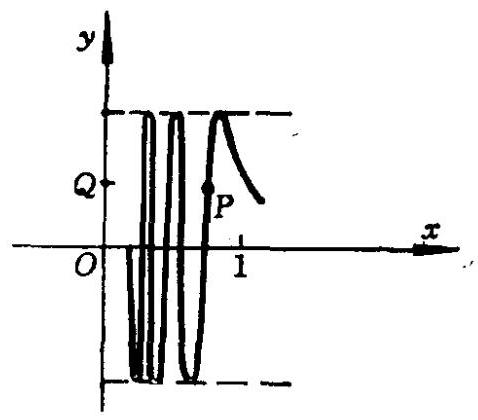
\includegraphics[max width=0.4\textwidth]{images/bo_d25ksc77aajc738obdgg_555_642_1424_478_420_0.jpg}
\end{center}
\hspace*{3em} 

图 10-12

定义映射 $f : \left\lbrack  {0,1}\right\rbrack   \rightarrow  {\mathbf{R}}^{2}$ 如下:
$$\forall x \in  \rbrack 0,1\rbrack ,f\left( x\right)  = \left( {x,\sin \frac{1}{x}}\right) \text{ , }$$

则映射 $f$ 连续. 由于 $\rbrack 0,1\rbrack$ 连通,故 $\left. {f\left( {\rbrack 0,1\rbrack }\right\rbrack   = A}\right)$ 是 ${\mathbf{R}}^{2}$ 的连通集,从而 $\bar{A}$ 也是连通的.

下面我们证明 $A$ 是道路连通的,而 $\bar{A}$ 不是道路连通的.

为此设 $P\left( {x,y}\right) ,Q\left( {{x}^{\prime },{y}^{\prime }}\right)  \in  A$ ,不妨设 $x < {x}^{\prime }$ . 则
$$f\left( x\right)  = P,f\left( {x}^{\prime }\right)  = Q.$$

$f$ 在 $\left\lbrack  {x,{x}^{\prime }}\right\rbrack$ 上的限制 ${\left. f\right| }_{\left\lbrack  x,{x}^{\prime }\right\rbrack  }$ 是连续映射,因此它是 $A$ 的联结 $P$ 与 $Q$ 的一条道路,故 $A$ 是道路连通集,

现在设 $P\left( {x,y}\right)  \in  A,Q\left( {0,{y}^{\prime }}\right)$ 为 $\bar{A}$ 在 $y$ 轴上的任意一点 (如图10-12所示). 我们来证明不可能存在 $\bar{A}$ 中联结 $P$ 与 $Q$ 的任何道路.

假设存在这样的一条道路 $\varphi  : \left\lbrack  {a,b}\right\rbrack   \rightarrow  \bar{A}$ ,使得 $\varphi \left( a\right)  = Q(0$ , $\left. {y}^{\prime }\right) ,\varphi \left( b\right)  = P\left( {x,y}\right)$ . 记 $\varphi \left( t\right)  = \left( {{\varphi }_{1}\left( t\right) ,{\varphi }_{2}\left( t\right) }\right)$ ,则 ${\varphi }_{1}\left( a\right)  = 0$ , ${\varphi }_{1}\left( b\right)  = x > 0$ . 令
$${t}_{0} = \inf \left\{  {t \in  \left\lbrack  {a,b}\right\rbrack   \mid  {\varphi }_{1}\left( t\right)  > 0}\right\}  .$$

由 ${\varphi }_{1}$ 的连续性及 ${t}_{0}$ 的定义知, ${t}_{0} < b$ 且 ${\varphi }_{1}\left( {t}_{0}\right)  = 0$ . 于是存在 ${t}_{n} > {t}_{0}$ , 且 ${t}_{n} \rightarrow  {t}_{0}$ ,使 ${\varphi }_{1}\left( {t}_{n}\right)  > 0,\mathop{\lim }\limits_{{n \rightarrow   + \infty }}{\varphi }_{1}\left( {t}_{n}\right)  = 0$ . 由此推得 ${\varphi }_{2}\left( {t}_{0}\right)  =$  $\mathop{\lim }\limits_{{n \rightarrow   + \infty }}\sin \frac{1}{{\varphi }_{1}\left( {t}_{n}\right) }$ ,这不可能,因该极限不存在. 故 $\bar{A}$ 非道路连通.

附注 虽然定理 ${10} \cdot  6 \cdot  8$ 的逆不成立,但对 ${\mathbf{R}}^{n}$ 中的开集来说, 连通与道路连通是等价的. 因为道路连通开集必是连通的, 故我们只需证明 ${\mathbf{R}}^{n}$ 的连通开集是道路连通的. 实际上我们可以证明所谓的 “折线连通性”,为此我们首先介绍 ${\mathbf{R}}^{n}$ 中的折线与 “折线连通”的概念.

定义 设 $U \subset  {\mathbf{R}}^{n}$ 是任一非空集合.

1) 一条道路 $\varphi  : \left\lbrack  {a,b}\right\rbrack   \rightarrow  U$ 称为折线,如果像集 $\varphi \left( \left\lbrack  {a,b}\right\rbrack  \right)$ 是有限条线段的并.

2) $U$ 称为是折线连通的,如果 $U$ 中任意两点 $x$ 与 $y$ 都可以用 $U$ 中的一条折线联结.

定理 ${10} \cdot  6 \cdot  9\;{\mathbf{R}}^{n}$ 的任一连通开集是折线连通的.

证明 设 $U$ 是 ${\mathrm{R}}^{n}$ 的任一连通开集, ${x}_{0} \in  U$ . 定义集合 $A$ 与 $B$ 如下:

$A = \left\{  {x \in  U \mid  \text{ 可用 }U\text{ 中的一折线联结 }{x}_{0}\text{ 与 }x}\right\}  ,$

$B = U - A,$

于是
$$A \cap  B = \varnothing ,A \cup  B = U.$$

下面我们来证明 $A$ 与 $B$ 是 ${\mathbf{R}}^{n}$ 中的两个开集.

因为 ${x}_{0} \in  A$ ,故 $A \neq  \varnothing$ ,任取 $x \in  A$ . 由于 $x \in  U$ ,故存在 $\delta  > 0$ 使得 $B\left( {x,\delta }\right)  \subset  U.\;\forall y \in  B\left( {x,\delta }\right) ,x$ 与 $y$ 可用一折线 ${l}_{1}$ 联结,而 ${x}_{0}$ 与 $x$ 可用折线 ${l}_{2}$ 联结,故 ${x}_{0}$ 与 $y$ 可用折线 ${l}_{2} \cup  {l}_{1}$ 联结,从而 $y \in  A$ , 即 $B\left( {x,\delta }\right)  \subset  A$ ,因此 $A$ 是 ${\mathbf{R}}^{n}$ 的非空开集.

如果 $B = \varnothing$ ,则 $U = A$ 为折线连通集.

假设 $B \neq  \varnothing$ ,下面我们来证明 $B$ 也是 ${\mathbf{R}}^{n}$ 的开集. 设 $b \in  B$ ,由于 $b \in  U$ ,故存在 $\eta  > 0$ 使得 $B\left( {b,\eta }\right)  \subset  U$ . 如果存在 $y \in  B\left( {b,\eta }\right)$ , 使得 ${x}_{0}$ 与 $y$ 可用折线 ${L}_{1}$ 联结,则由于 $y$ 与 $b$ 可用折线 ${L}_{2}$ 联结知, ${x}_{0}$ 与 $b$ 可用折线 ${L}_{1} \cup  {L}_{2}$ 联结,从而 $b \in  A$ ,这与 $b \in  B$ 矛盾. 故 $B\left( {b,\eta }\right)  \subset  B$ ,即 $B$ 为 ${\mathbf{R}}^{n}$ 的开集. 这时(A, B)形成 $U$ 的一个分裂, 这与 $U$ 的连通性假设矛盾,故必有 $B = \varnothing$ ,定理证毕.

例11 例 10 中的集合 $A$ 虽然是道路连通的,但不是折线连通的.

\section*{习 题}

1. 证明: $\rbrack  - \infty ,b\left\lbrack  \text{ 与 }\right\rbrack  a, + \infty \lbrack$ 是 $\mathrm{R}$ 的连通集,

2. 证明: ${\mathrm{R}}^{2}$ 的下述集合
$$A = \left\{  {\left( {x,y}\right)  \in  {\mathbf{R}}^{2} \mid  y = 0}\right\}   \cup  \left\{  {\left( {x,y}\right)  \in  {\mathbf{R}}^{2} \mid  x > 0,y = \frac{1}{x}}\right\}$$

是非连通的.

3. 设 $I \subset  R$ 是任一连通集,它至少包含两个点. 证明: $I$ 是 $R$ 的一个区间.

4. 设(X, d)是任一度量空间. 证明:(X, d)是非连通的,当且仅当存在一个连续映射 $f : X \rightarrow  \mathrm{R}$ 及点 $a,b \in  \mathrm{R}$ 使得 $f\left( X\right)  = \{ a,b\} \left( {a \neq  b}\right)$ .

5. 证明: 若度量空间(X, d)连通并且至少包含两个点,则存在连续映射 $f : X \rightarrow  \left\lbrack  {0,1}\right\rbrack$ 使得 $f\left( X\right)  = \left\lbrack  {0,1}\right\rbrack$ .

6. 设 $\left\langle  {A}_{n}\right\rangle$ 是度量空间(X, d)的一列连通子集,使得 $\forall n \in  \mathbf{N},{A}_{n} \cap$  ${A}_{n + 1} \neq  \varnothing$ ,证明 $\mathop{\bigcup }\limits_{{n = 1}}^{\infty }{A}_{n}$ 也是连通集.

7. 设 ${\left\{  {A}_{\lambda }\right\}  }_{\lambda  \in  \Lambda }$ 是度量空间(X, d)的任一连通集族, $A$ 是(X, d)的连通子集,使得 $\forall \lambda  \in  \Lambda ,A \cap  {A}_{\lambda } = \varnothing$ ,证明 $A \cup  \left( {\mathop{\bigcup }\limits_{{\lambda  \in  \Lambda }}{A}_{\lambda }}\right)$ 也是连通集.

8. 设 $D = \left\{  {\left. \frac{1}{n}\right| \;n \in  \mathbf{N}}\right\}$ ,定义 ${\mathbf{R}}^{2}$ 中的两个集合 $A$ 、 $B$ 如下:
\begin{align*}
	&A = \left( {\left\lbrack  {0,1}\right\rbrack  \times \{ 0\} }\right)  \cup  \left( {D \times  \left\lbrack  {0,1}\right\rbrack  }\right)  \cup  \left( {\{ 0\}  \times  \left\lbrack  {0,1}\right\rbrack  }\right) ,\\
	&B = \left( {\left\lbrack  {0,1}\right\rbrack  \times \{ 0\} }\right)  \cup  \left( {D \times  \left\lbrack  {0,1}\right\rbrack  }\right)  \cup  \{ \left( {0,1}\right) \} .
\end{align*}

$A$ 称为梳空间, $B$ 称为缺边梳空间.

1) 画出 $A$ 与 $B$ 的图形.

2) 证明: $A$ 是道路连通的及折线连通的.

3) 证明: $B$ 是连通的,但不是道路连通的.

9. 证明下述各结论:

1) $\forall n > 1,{R}^{n}$ 与 $R$ 不同胚, ${S}^{n - 1}$ 与 ${S}^{1}$ 不同胚.

2) $\forall n > 1,{\mathrm{R}}^{n}$ 的全体有理点 (即它的 $n$ 个坐标全为有理数) 的集合是不连通的; ${R}^{n}$ 的非有理点 (即它的 $n$ 个坐标中至少有一个是无理数) 的集合是折线连通的.

3) 设 $D$ 是 ${\mathrm{R}}^{n}$ 的任一可数集 $\left( {n > 1}\right)$ ,则 ${\mathrm{R}}^{n} - D$ 是道路连通的.

10. 证明: 函数 $f : R \rightarrow  R$ 是单调的充分必要条件是: $\forall y \in  R,{f}^{-1}\left( y\right)$ 是 $\mathrm{R}$ 的连通子集.

11. 设 $a > 0,f : {\mathrm{R}}^{n} \rightarrow  {\mathrm{R}}^{n}$ 是任一连续映射,它满足下述条件:
$$\forall x,y \in  {\mathrm{R}}^{n},d\left( {f\left( x\right) ,f\left( y\right) }\right)  \geq  {ad}\left( {x,y}\right) .$$

证明: $f\left( {R}^{n}\right)  = {R}^{n}$ .

12. 设 $\left( {X,d}\right) ,\left( {Y,D}\right)$ 是两个度量空间, $f : X \rightarrow  Y$ 是任一连续满射使得 $\forall y \in  Y,{f}^{-1}\left( y\right)$ 是连通集. 证明: 若 $B \subset  Y$ 是连通集,则 ${f}^{-1}\left( B\right)$ 也是连通集.

13. 设(X, d)是任一度量空间, $x,y \in  X,\varepsilon  > 0$ . 我们称 $X$ 的一个有限点序列 $\left\langle  {{x}_{1},{x}_{2},\cdots ,{x}_{n}}\right\rangle$ 是从 $x$ 到 $y$ 的一个 $\varepsilon$ 一有限链,如果下述性质成立:
$$x = {x}_{1},y = {x}_{n},d\left( {{x}_{i},{x}_{i + 1}}\right)  < \varepsilon \;\forall i = 1,2,\cdots ,n - 1.$$

证明:

1) 若(X, d)连通,则 $\forall x,y \in  X,\forall \varepsilon  > 0$ ,存在从 $x$ 到 $y$ 的 $\varepsilon$ 一有限链.

2) 若(X, d)是紧的,并且 $\forall x,y \in  X,\forall \varepsilon  > 0$ ,存在从 $x$ 到 $y$ 的 $\varepsilon$ 一有限链,则(X, d)是连通的.
